\documentclass[11pt,a4paper]{article}
\usepackage[margin=1in]{geometry}
\usepackage[T1]{fontenc}
\usepackage[utf8]{inputenc}
\usepackage{lmodern,microtype}
\usepackage{amsmath,amssymb,amsthm,mathtools}
\usepackage{graphicx,booktabs,tabularx,array,longtable}
\usepackage[authoryear,round]{natbib}
\usepackage{xurl}
\usepackage[hidelinks]{hyperref}
\usepackage[nameinlink,noabbrev]{cleveref}
\usepackage{enumitem}
\ifdefined\reviewmode\usepackage{lineno}\fi
\graphicspath{{figures/}{archive/v7_3/manuscript/figures/}}
\setlength{\emergencystretch}{2em}
\setlength{\tabcolsep}{5pt}
\renewcommand{\arraystretch}{1.14}
\newcolumntype{Y}{>{\raggedright\arraybackslash}X}
\newtheorem{proposition}{Proposition}
\newtheorem{corollary}[proposition]{Corollary}
\newtheorem{lemma}[proposition]{Lemma}
\newtheorem{productioncorollary}{Corollary}[proposition]
\crefname{productioncorollary}{corollary}{corollaries}
\Crefname{productioncorollary}{Corollary}{Corollaries}
\theoremstyle{definition}\newtheorem{definition}{Definition}
\newcommand{\CITH}{\textsc{CITH}}
\newcommand{\dd}{\,\mathrm{d}}
\newcommand{\Rogue}{R_{\mathrm{rogue}}}
\newcommand{\Sq}{\mathcal S_q}
\newcommand{\Aauto}{\mathcal A}

% BEGIN expanded result_macros.tex
\newcommand{\DesignLogMin}{20.31}
\newcommand{\DesignLogMax}{21.07}
\newcommand{\DesignLinearMin}{10.99}
\newcommand{\DesignLinearMax}{11.82}
\newcommand{\DynamicThreshold}{0.4091}
\newcommand{\DynamicOutward}{3.7559}

% END expanded result_macros.tex


% BEGIN expanded v73_result_macros.tex
% Generated by code/validate_v73.py; original result_macros.tex is unchanged.
\newcommand{\ReverseStaticTerm}{+0.03899}
\newcommand{\ReverseFutureTerm}{-0.06310}
\newcommand{\ReverseTotalTerm}{-0.02411}
\newcommand{\ReverseStaticX}{6}
\newcommand{\ReverseDynamicX}{0}

% END expanded v73_result_macros.tex

\title{Why Should They Stop Expanding?\\[3pt]
\large Computational Growth, Tipping Budgets, and the Uniformity Problem}
\author{Hyeonjun Joo\\[3pt]\normalsize Independent Researcher, Republic of Korea\\
\normalsize\href{mailto:jonejoo0805@gmail.com}{jonejoo0805@gmail.com}}
\date{13 October 2026}
\hypersetup{pdftitle={Why Should They Stop Expanding? CITH v8},pdfauthor={Hyeonjun Joo}}
\begin{document}\maketitle
\begin{abstract}
Computational abundance does not by itself remove the incentive to expand.
We develop a resource-allocation theory that separates physical budget
growth, computational efficiency, and the creation of valued virtual worlds.
With logarithmic value, concave local production, bounded external prices,
and persistent residual external motives, unbounded budgets exclude
permanent all-inward allocation regardless of productivity. A tight
production-independent floor yields a unique tipping budget; an explicit
resource-acquisition process has a unique boundary between eventual inward
investment and outward lock-in. Optimizing observation and dormant backups
changes the relevant condition from all-inward investment to no replication.
An expected-catastrophe model shows why protecting a growing internal value
can preserve a seed-backup incentive. A free-world-number lemma connects
specified population ethics to value curvature, and a verified
infinite-horizon benchmark separates current computational returns from
future resource growth. Subjective-delay discounting can weaken remote
returns, but must account for the timing of descendant production and the
risk cost of delayed protection. Finally, a marked-origin model quantifies
the small expansionist tail compatible with a chosen null-arrival likelihood
when potential exposure is large. These results specify the resource,
service-substitution, and timing tests for an inward scenario while identifying
alternative routes and failures. They do not estimate extraterrestrial
preferences, establish indefinite local engineering feasibility, or infer
low detectability from inward allocation.
\end{abstract}
\noindent\textbf{Keywords:} Fermi paradox; computational inward transition;
resource allocation; replication; population ethics; technosignatures.

% BEGIN MAIN TEXT
\section{Introduction}
\label{sec:introduction}
The capacity to cross interstellar distances does not settle whether a
civilization will keep paying to do so. Yet an inward explanation of the
Fermi paradox faces a stronger objection than this elementary distinction:
resource growth itself can renew the incentive to expand. A civilization
that values additional computation need not exhaust its ambitions before
acquiring another star. If extensive industry produces resources and
independent options that intensive local investment cannot supply cheaply,
better computers may strengthen neither local sufficiency nor the decision
to remain local. The computational inward transition hypothesis (\CITH)
therefore needs a boundary that expansion can cross, not a verbal claim
that virtual experience is attractive.

Expansion arguments associated with \citet{Hart1975} and \citet{Tipler1980}
connect technological capability to persistent settlement or self-replicating
activity. The wider assumptions behind the Great Silence were surveyed by
\citet{Brin1983}. Settlement dynamics, finite site lifetimes, and spatial
heterogeneity complicate complete occupation \citep{NewmanSagan1981,CarrollNellenback2019}.
They do not make launch behaviour irrelevant: an expansionist lineage can
have consequences far beyond its original population. Our question is
whether an internal computational alternative removes the incentive to
create that lineage, and whether removing it in many civilizations is enough
to explain no arrival in a specified region.

The answer developed here begins against the strong hypothesis. With
logarithmic computational value, concave local production, bounded external
prices, and a positive residual external motive, unbounded physical budgets
eventually exclude all-inward allocation, whatever local computational
productivity does. This result treats efficiency and physical resources as
different quantities. A processor improvement changes the useful service
obtained from a fixed energy or material allocation; access to another
resource base changes the allocation that can be made. Conflating these
changes would remove precisely the outward pressure that the model tests.

\subsection{Contribution and organizing argument}
The contribution has four connected parts. First, a common corner criterion
yields a tight production-independent floor and a unique tipping budget
under logarithmic value. An explicit resource-acquisition process has a
unique initial-productivity boundary separating eventual inward investment
from outward lock-in, with a critical path approaching the tipping budget.
Second, optimizing non-replicating observation and dormant backups changes
the relevant corner and replaces gross project prices by opportunity costs
net of substitute services. A growing-budget construction shows that the two corners can even have opposite persistence conclusions. A catastrophe model then derives the resilience
premium from value at risk rather than assigning it freely. Third, a
free-world-number margin connects a specified population ethic to value
curvature, while an infinite-horizon benchmark and subjective-delay
inequalities make continuation returns explicit. Finally, a marked-origin
arrival model quantifies how small the expansionist tail must be when
potential arrival exposure is large.

These results organize a particular inward scenario around three tests:
a viable resource path that stays on the appropriate side of an incentive
boundary, credible non-replicating ways of satisfying external information
and resilience motives, and sufficiently weak time-adjusted returns on
replication. The tests must hold together in a scenario relying on all
three mechanisms. They are not universal necessary conditions for every
possible inward civilization. Slower marginal-value decay, vanishing
external preferences, strongly increasing local returns, or rising external
prices supply different routes. The model proves conditional exclusions
and existence results, not a universal evolutionary destiny. Its strongest
negative conclusion is correspondingly precise: within the logarithmic,
concave-production benchmark, productivity alone cannot defeat a persistent
residual motive when the physical budget grows without bound.

The corner calculation uses standard concave optimization. Its contribution
is not a new first-order optimality theorem. The additional theory lies in
sharp feasibility across production functions, the pathwise obstruction,
the unique basin boundary, the exact scope and failure of an exponential
endpoint test, and the links between service substitution, intertemporal
returns, and population exposure. Each link has its own assumptions. In
particular, a sufficient condition for one civilization to stop new
investment is not a theorem that all existing autonomous descendants stop
replicating. A population argument must keep their exposure in the record.

\subsection{What is inherited from prior work}
Computational and postbiological civilizations are established subjects,
not ideas introduced by this paper \citep{Dick2003,CirkovicBradbury2006}.
\citet{Smart2012} describes movement toward dense internal scales. Our
increasing-returns result supplies a resource-response condition against
which that kind of mechanism can be tested. It does not import the stronger
claim that advanced civilizations invariably leave the observable universe.
Bradbury's Matrioshka-brain manuscript describes stellar computation and
nested heat-use architectures \citep{Bradbury1999}; the thermal calculation
below is a deliberately smaller bridge between allocation and search,
not a proposal of that architecture.

Aestivation instead concerns when to compute \citep{Sandberg2017}. The
thermodynamic objection of \citet{BennettHansonRiedel2019} emphasizes that
available entropy reservoirs must be specified before efficiency advantages
are inferred. Our latency comparison concerns delayed external returns
relative to ongoing internal activity, and does not assume that waiting
for a colder universe is optimal. Sustainability and homeostatic proposals
address other reasons expansion might end \citep{HaqqMisraBaum2009,WongBartlett2022}.
They can coexist with the allocation mechanism but do not prove its
thresholds. Conversely, self-replicating resource acquisition
\citep{ArmstrongSandberg2013} and population-total welfare
\citep{Bostrom2003Waste} are direct counterpressures. They are included as
cases in which outward investment can remain attractive.

\subsection{Three meanings of inwardness}
We reserve \emph{all-inward allocation} for zero new expenditure on resident,
industrial, and observation projects. \emph{No replication} instead permits
observation and dormant backups, while setting new reproducing capacity
to zero. \emph{Low detectability} is an observational property and can hold
or fail under either allocation. These definitions also distinguish a
civilization's current investment from the continued activity of earlier
launches. A society may stop launching because its distant industry is
already reproducing effectively; that is not an explanation of silence.

The paper proceeds through these distinctions rather than treating every
external project as colonization. The model first separates physical
support from economic preference, then identifies the corner and its
persistence conditions. Residual motives and latency determine whether
those conditions survive a more explicit account of services and time.
The population calculation finally asks how much outward or leaked activity
a chosen null likelihood tolerates. Detailed workload examples, the paired
sensitivity ensemble, and the original two-period construction are in the
supplement. Their numerical values are preserved as implementation checks,
not used as a prior over unknown civilizations.

\section{Model: workload, resources, and value}
\label{sec:support}
\label{sec:allocation}
\subsection{Experiential substitution and implemented states}
Let $q\in[0,1]$ denote decision-relevant experiential fidelity and let
$\sigma(q)\in[0,1]$ be an increasing substitution map. For a residence
project with experiential benefit $E(n)$ and residual value $X(n)$,
\begin{equation}
 B_{\rm phys}(n,q)=[1-\sigma(q)]E(n)+X(n).
 \label{eq:experiential}
\end{equation}
Perfect substitution removes the first term, not external facts, materials,
geographical protection, or strategic options. For a discrete project with
substitutable value $e_j$, residual value $x_j$, and incremental resource
cost valued at $c_j$, the net comparison is
\begin{equation}
 \Delta_j(q)=[1-\sigma(q)]e_j+x_j-c_j.\label{eq:premium}
\end{equation}
A positive reality premium need not cover its opportunity cost. The
continuous model below specializes to $\sigma(q)=q$. This is a statement
about a decision-maker's substitution, not about the metaphysical identity
of a physical event and its simulation.

A regular hierarchy with branching factor $b\geq2$ and finite integer
depth $d\geq0$ contains
\begin{equation}
 W_d=\sum_{j=0}^{d}b^j=\frac{b^{d+1}-1}{b-1}.\label{eq:worlds}
\end{equation}
For per-world service requirement $u_k>0$, efficiency $\eta_k>0$, and
capacity $K_k$, homogeneous support requires
\begin{equation}
 D_k(d)=u_kW_d/\eta_k\leq K_k\quad\hbox{for every service }k.
 \label{eq:resource}
\end{equation}
Processing, state storage, heat rejection, and material replacement are
separate constraints. Their units cannot be added without an explicit
conversion. Cumulative consumption and available stocks must refer to the
same horizon; instantaneous power is not a lifetime energy supply.

\begin{lemma}[Finite-depth support frontier]
\label{prop:depth}
Let $Q=\min_kK_k\eta_k/u_k$. If $Q\geq1$, the largest feasible depth is
\begin{equation}
 d_{\max}=\left\lfloor\log_b[1+(b-1)Q]-1\right\rfloor.
 \label{eq:depth-bound}
\end{equation}
If $Q<1$, even the root world is infeasible at the specified workload.
\end{lemma}
\begin{proof}
The intersection of the service constraints is $W_d\leq Q$. Substituting
the geometric sum, taking the increasing base-$b$ logarithm, and restricting
to non-negative integers gives the result.
\end{proof}

For fixed per-world workloads,
$D_k(d+1)/D_k(d)=b+1/W_d\to b$. With $C_d=cW_d$ and logarithmic
value, the increment is
$\ln\{[1+c(bW_d+1)]/[1+cW_d]\}\to\ln b$.
These limits divide numerator and denominator by $W_d$. Recursion
therefore multiplies implemented demand while producing only a bounded
increment in logarithmic value per additional level. A rule that generates
unbounded depth is not an implementation of infinitely many simultaneous
independent states. Reusing code also does not erase distinct stored
histories. Scheduling fewer active worlds can save update work while
leaving a growing persistent-memory bill.

On a specified horizon $[0,T]$, define
\begin{equation}
 \chi_T=\sup_{0\leq t\leq T}\max_k\frac{D_k(t)}{K_k(t)}.
 \label{eq:chi}
\end{equation}
Local physical sufficiency means $\chi_T\leq1$. For a ratio
$\chi_{k0}\exp[(g_{D,k}-g_{K,k})t]$ initially below one and a positive
growth-rate difference, its crossing time is
\begin{equation}
 T_k=\frac{\ln(1/\chi_{k0})}{g_{D,k}-g_{K,k}}.\label{eq:crossing}
\end{equation}
This follows by solving for a ratio of one. It separates a successful
finite interval from a permanently feasible implementation. The archived
examples and their first memory failure are retained in the supplement.
The new results do not assume those examples establish indefinite support.

\subsection{A common resource budget}
Let $z,x,y,w\geq0$ be local investment, resident infrastructure,
industry-only capacity, and observation-only capacity. With local
investment as numeraire,
\begin{equation}
 z+p_nx+p_hy+p_mw\leq B,\qquad p_j>0,
 \label{eq:budget}
\end{equation}
where $B>0$ unless the degenerate zero-budget case is expressly mentioned.
A support constraint and an allocation constraint answer different
questions. A physically sufficient local path can still lose to a more
valuable external use, while an attractive local allocation can fail a
memory or heat requirement. Their conjunction, rather than either
calculation alone, describes an implementable inward path.

\label{sec:production}

The planning horizon and the resource numeraire are fixed. Let
$B_{\rm res}$ be physical resources available during that horizon and let
$b_{\rm ref}>0$ be a fixed reference amount. The budget coordinate is
$B=B_{\rm res}/b_{\rm ref}$; local investment and project prices use the
same resource unit. Thus $p_jx_j$ and $z$ are resource expenditures, whereas
$x,y,w$ are dimensionless increments of project capacity. Similarly,
$C=C_{\rm useful}/c_{\rm ref}$ uses a fixed computational-service unit
$c_{\rm ref}>0$. In particular, logarithms take dimensionless arguments.
An efficiency improvement changes the production coefficient $a$, not
$B$, unless it also changes the physical resources actually available.
Other physical services retain the separate constraints in \cref{eq:chi}.

The cumulative indices $n=1+x$, $h=1+x+y$, and $m=1+x+y+w$ retain the
residence, industry, and observation accounting of the model. Useful
computation and utility are
\begin{align}
 C&=C_0+a\ell(z)+G_n(x)+G_h(y),\label{eq:compute}\\
 U&=F(C)+(1-q)E(x)+\epsilon_RR(x+y)
       +\epsilon_II(x+y+w).\label{eq:utility}
\end{align}
Here $a>0$, $C_0\geq0$, $q\in[0,1]$, and the residual weights are
non-negative. The functions $E,R,I$ are differentiable, non-decreasing,
and concave on the feasible domain. The functions $G_n,G_h$ are
continuous, non-decreasing, and concave, with $G_j(0)=0$ and finite right
derivatives $G_j'(0)=r_j\geq0$. Set $r_m=0$. Local production is continuous
and non-negative on $[0,B]$, with $\ell(0)=0$, and has a positive finite
left derivative at $B$ and $\ell(B)>0$. Whenever global concavity is
invoked, $\ell$ is also concave on this interval. These assumptions do
not require a derivative at zero. The baseline is
$\ell(z)=\ln(1+z)$ and $G_j(v)=r_jv$.

We use the shifted-isoelastic computational value
\begin{equation}
 F_\eta(C)=
 \begin{cases}
 [(1+C)^{1-\eta}-1]/(1-\eta),&\eta\ne1,\\
 \ln(1+C),&\eta=1,
 \end{cases}
 \qquad \eta\geq0,
 \label{eq:isoelastic}
\end{equation}
so that $F_\eta'(C)=(1+C)^{-\eta}$, $F_\eta(0)=0$, and
$F_\eta'(0)=1$. The common marginal-value normalization makes the
residual weights comparable across this family. The value-curvature
parameter $\eta$ is distinct from the service-efficiency factors $\eta_k$.
Recursive description alone does not determine a welfare functional.

The residual slopes at the all-inward corner are
\begin{align}
 S_n&=(1-q)E'(0)+\epsilon_RR'(0)+\epsilon_II'(0),\nonumber\\
 S_h&=\epsilon_RR'(0)+\epsilon_II'(0),&
 S_m&=\epsilon_II'(0).
 \label{eq:slopes}
\end{align}
Write $d_0=1+C_0\geq1$ and define
\begin{equation}
 \Omega=a\ell(B),\qquad
 \Gamma(B)=\frac{\ell(B)}{\ell'(B)}.
 \label{eq:omega-gamma}
\end{equation}
The first quantity is new local computational output at the corner;
the second is a resource-scale measure of production curvature.
Changing the multiplicative normalization of $\ell$ and compensating in
$a$ changes neither quantity. Throughout, all-inward allocation means
zero new expenditure in every external direction. It is stronger than
zero new replication, since observation can be external without
replicating.

\subsection{World creation and computational-value curvature}
\label{sec:world-value}
A generative architecture does not select a welfare functional, but a free
margin in the number of worlds changes the value of additional computation.
To expose that margin, let $C_{\rm tot}\geq u>0$ be service available to
worlds, let each world receive $c\geq u$, and initially relax world count
to a real variable $W\geq1$. The constraint is $Wc=C_{\rm tot}$. The
exponent $\theta\in[0,1]$ values world population; the elasticity
$\alpha\in(0,1]$ values resources within a world. This distinction is
between two margins of valuation, not between simulated and physical
persons.

\begin{lemma}[A free world-number margin]
\label{lem:world-curvature}
For the continuous relaxation,
\begin{equation}
 \max_{Wc=C_{\rm tot},\,W\geq1,\,c\geq u}W^\theta c^\alpha
 =\begin{cases}
 u^{\alpha-\theta}C_{\rm tot}^{\theta},&\theta>\alpha,\\
 C_{\rm tot}^{\alpha},&\theta\leq\alpha.
 \end{cases}
 \label{eq:world-value}
\end{equation}
Thus the value exponent is $v=\max(\theta,\alpha)>0$. Writing
$C_{\rm tot}=u(1+C)$ and normalizing the value at the mandatory root
as $[V(u(1+C))/V(u)-1]/v$ gives exactly $F_{1-v}(C)$.
For the separate specification $W^\theta\ln(c/u)$, $\theta=0$ gives
$\ln(C_{\rm tot}/u)$, while $\theta>0$ gives
$(C_{\rm tot}/u)^\theta/(\exp(1)\theta)$ only once
$C_{\rm tot}\geq u\exp(1/\theta)$.
\end{lemma}
\noindent\emph{Proof sketch.}
Substitution of $W=C_{\rm tot}/c$ reduces the power case to the sign
of $\alpha-\theta$. In the logarithmic case, optimize
$\exp[\theta\ln(C_{\rm tot}/u)-\theta v_c]v_c$ over
$0\leq v_c\leq\ln(C_{\rm tot}/u)$. The full proof, ties, and the
integer-world correction are in \cref{app:world-proof}.

At $\theta=\alpha$ every feasible continuous split ties. With integer
world counts and $\theta>\alpha$, the exact value becomes
$C_{\rm tot}^\alpha\lfloor C_{\rm tot}/u\rfloor^{\theta-\alpha}$;
it has the same asymptotic exponent, not the same differentiable function.
A regular recursive hierarchy restricts the available counts further but
preserves this exponent. The shifted smooth family is therefore exact for
the stated relaxation, not for discrete launches or indivisible worlds.

Average-log valuation is one interpretation of the baseline $\eta=1$.
It is not forced by computational sophistication. Total-log valuation
with freely increasing world count instead has linear asymptotic value,
and the power model with $\theta=1$ has linear value exactly. At
$\eta=0$ the corner condition becomes
\begin{equation}
 p_ja\ell'(B)\geq r_j+S_j.
 \label{eq:totalist-corner}
\end{equation}
For logarithmic local production, densification must satisfy
$a/(1+B)\geq\max_j(r_j+S_j)/p_j$. More valued lives can thus strengthen
the attraction of unused external resources rather than eliminate it.
This connects the opportunity-cost comparison to
\citet{Bostrom2003Waste}, without attributing the present production
function or equation to that paper.

Recursion supplies one implementation of an open-ended world-number
margin. Its analytical role is now explicit: admitting that margin and
specifying its population weight changes the induced value curvature.
A non-recursive implementation with the same feasible world counts has
the same implication. Recursion neither manufactures additional substrate
nor chooses $\theta$ on behalf of a civilization. The extensive world
margin, rather than nesting by itself, is the operative assumption.

\section{The inward corner}
\label{sec:inward}
\label{sec:threshold}

A corner criterion is useful only if it exposes the quantities that can
and cannot be changed by productivity. Temporarily allow any
differentiable, strictly increasing, concave $F$. At the corner define
\begin{align}
 C_L&=C_0+a\ell(B),&
 \lambda_L&=F'(C_L)a\ell'(B),\label{eq:local-return}\\
 D_j&=F'(C_L)r_j+S_j\qquad(j=n,h,m).
 \label{eq:external-return}
\end{align}

\begin{proposition}[The common corner criterion]
\label{prop:hub}
Under the model assumptions, a necessary condition for the all-inward
corner to be globally optimal is
$D_j\leq p_j\lambda_L$ for every direction. This condition is also
sufficient when $\ell$ is concave. For $F=F_\eta$, it is equivalent to
\begin{equation}
 \boxed{\frac{p_j}{\Gamma(B)}\geq
 \frac{r_j}{\Omega}
 +S_j\frac{(d_0+\Omega)^\eta}{\Omega}}
 \qquad(j=n,h,m).
 \label{eq:hub}
\end{equation}
Productivity enters this expression only through $\Omega$; $\Gamma$
depends on the production function and the budget, not on $a$.
Under concavity, strict inequalities in every direction make every
optimizer all-inward. Weak inequalities establish an inward optimum
but do not by themselves exclude tied external allocations.
\end{proposition}
\begin{proof}
Let $(v_n,v_h,v_m)=(x,y,w)$. Moving a small amount $v_j>0$ into direction
$j$ and reducing $z$ by $p_jv_j$ gives directional derivative
$D_j-p_j\lambda_L$. A positive derivative contradicts optimality.
If $\ell$ is concave, then $C$ is concave and composition with increasing
concave $F$ preserves concavity. Consequently,
\begin{align}
 U(z,x,y,w)-U(B,0,0,0)
 &\leq\lambda_L(z-B)+\sum_jD_jv_j\nonumber\\
 &\leq\sum_j(D_j-p_j\lambda_L)v_j.
 \label{eq:cornerproof}
\end{align}
This proves sufficiency and the strict statement. For $F_\eta$,
multiplication by $(d_0+\Omega)^\eta>0$ gives
$p_ja\ell'(B)\geq r_j+S_j(d_0+\Omega)^\eta$; division by
$\Omega>0$ gives \cref{eq:hub}.
\end{proof}

\begin{corollary}[The original all-inward criterion]
\label{prop:corner}
For $\ell(z)=\ln(1+z)$ and any differentiable, strictly increasing,
concave $F$, the all-inward corner is optimal exactly when
\begin{equation}
 D_j/p_j\leq\lambda_L\qquad(j=n,h,m).
 \label{eq:corner}
\end{equation}
\end{corollary}
\begin{proof}
The local logarithm is concave, so both directions of
\cref{prop:hub} apply. Its derivatives give precisely
\cref{eq:local-return,eq:external-return} with
$\ell'(B)=1/(1+B)$.
\end{proof}

\begin{corollary}[Adding hard support constraints]
\label{cor:feasibility}
If an additional physical feasibility restriction retains the corner,
the criterion $D_j\leq p_j\lambda_L$ remains sufficient under
concavity, as does \cref{eq:hub} for $F_\eta$. Necessity is guaranteed
when each small budget-transfer direction used in the proof remains
admissible. Without that condition, necessity need not hold.
\end{corollary}
\begin{proof}
An optimum over a set is an optimum over any subset containing it.
The necessity argument requires exactly the indicated feasible
perturbations; without them it need not apply.
\end{proof}

\begin{productioncorollary}[The tight logarithmic floor]
\label{cor:production-growth}
Let $\eta=1$ and let $\ell$ be concave. Then
\begin{equation}
 \Gamma(B)\geq B,
 \label{eq:tight-floor}
\end{equation}
with equality if and only if $\ell$ is linear on $[0,B]$.
Every direction with $S_j>0$ requires
$p_j>S_j\Gamma(B)\geq S_jB$ at any finite $a$.
Conversely, for fixed finite $B,d_0,p_j,r_j,S_j$, some concave local
production function and finite $a>0$ make the corner optimal if and
only if $p_j>S_jB$ in every direction with $S_j>0$.
Linear local production provides a witness. Directions with $S_j=0$
retain their computational-return condition but introduce no residual
floor.
\end{productioncorollary}
\noindent\emph{Proof sketch.}
The tangent to a concave production function at $B$ lies above its
value at zero. Equality forces coincidence with the chord on the whole
interval. For the converse use $\ell(z)=z$ and take
$a>\max_j(r_j+d_0S_j)/(p_j-S_jB)$.
The complete proof, including zero slopes, is in \cref{app:floor-proof}.

\begin{corollary}[Logarithmic productivity thresholds]
\label{lem:production}
\label{prop:threshold}
For $\eta=1$ and concave $\ell$, the exact test is
\begin{equation}
 p_j\geq S_j\frac{\ell(B)}{\ell'(B)}
       +\frac{r_j+d_0S_j}{a\ell'(B)}.
 \label{eq:general-production}
\end{equation}
When $p_j>S_j\Gamma(B)$ in every nontrivial direction,
\begin{equation}
 a\geq a_{\rm crit}^{\ell}(B):=
 \max_{j:r_j+S_j>0}
 \frac{r_j+d_0S_j}{p_j\ell'(B)-S_j\ell(B)}
 \label{eq:acrit-general}
\end{equation}
is necessary and sufficient. The maximum over an empty set is zero.
If a nontrivial denominator is non-positive, no finite $a$ suffices.
For $\ell(z)=\ln(1+z)$, set $L=\ln(1+B)$ and recover
\begin{align}
 H_j&=(1+B)LS_j,& A_j&=(1+B)(r_j+d_0S_j),\label{eq:HA}\\
 p_j&\geq H_j+A_j/a,\label{eq:exact}\\
 a_{\rm crit}&=\max_{j:A_j>0}\frac{A_j}{p_j-H_j}.
 \label{eq:acrit}
\end{align}
Thus the general criterion contains both the original production test
and its logarithmic threshold.
\end{corollary}
\begin{proof}
Expand the $\eta=1$ term in \cref{eq:hub} and use
$\Omega=a\ell(B)$. The numerator in \cref{eq:acrit-general} is
positive exactly in nontrivial directions, so rearrangement is valid
exactly for positive denominators. If it is zero, then $r_j=S_j=0$.
Substitution of $\ell'(B)=1/(1+B)$ gives the last three equations.
\end{proof}

The supporting-hyperplane argument is standard
\citep[chapters 3--5]{BoydVandenberghe2004}. The substantive restriction
is the sharp residual floor: no concave redesign of local production
can reduce it below $S_jB$. Improvements in the level of computation
cannot remove this obstruction at logarithmic value.


\subsection{What the floor compares}
The floor is a relative-value statement. An additional unit of a project
can continue to provide independent information or geographical insurance
while the value of more local computation declines. Raising productivity
increases the level of local computation and its physical marginal product
at once. Under logarithmic value these effects partly cancel: the limiting
local marginal utility is $\ell'(B)/\ell(B)=1/\Gamma(B)$, not infinity.
Consequently a fixed external residual slope can remain competitive even
when remote computational production becomes negligible in the comparison.
This limit follows directly by dividing the logarithmic local marginal
utility by $a$ in numerator and denominator.

The distinction also explains the role of existing computation. Increasing
$C_0$ at fixed new-investment technology does not change the asymptotic
floor, but increases the finite-productivity term $d_0S_j$ in
\cref{eq:general-production}. A civilization with more existing useful
service need not place more marginal value on further service. When all
residual slopes are zero, by contrast, $C_0$ and the choice of increasing
$F$ do not affect the computational allocation: maximizing utility is
then equivalent to maximizing $C$. The pure-computation formula in
\cref{eq:budgetcrit} isolates that case. This is why an argument based
only on the attractiveness of virtual experience omits an independent
resource-allocation comparison.

Neither the floor nor the tipping budget measures a physical maximum
number of worlds. They specify when an additional external option beats
a marginal local use under the chosen objective. A system can be physically
capable of supporting its present workload while economically preferring
more territory. It can also prefer inward investment that fails an
independent support requirement. In an application the service ratios and
the allocation inequalities must therefore be evaluated on the same
resource history, rather than selecting a favourable budget for one and a
favourable efficiency for the other. The joint archived example demonstrates
compatibility on a finite interval; the persistence results determine what
additional conditions are needed beyond it.

A dimensionless robustness diagnostic is
\begin{equation}
 \rho=\max_j\frac{H_j+A_j/a}{p_j}.
 \label{eq:rho}
\end{equation}
The corner is inward when $\rho\leq1$. If every external price is multiplied by $\kappa>0$ while other terms are held fixed, the corner survives exactly when $\kappa\geq\rho$. Thus reporting $\rho$ identifies how much a conclusion depends on proximity to a threshold. This is conditional price sensitivity, not a distribution over unknown technologies.

\subsection{Analytical phase boundary}
For logarithmic value, define
\begin{equation}
 \xi_j=\frac{H_j}{p_j},\qquad
 \zeta_j=\frac{A_j}{p_ja}.
 \label{eq:phase-coordinates}
\end{equation}
The exact phase boundary is $\xi_j+\zeta_j=1$. All-inward allocation
requires $\xi_j+\zeta_j\leq1$ for \emph{every} direction.
If $\xi_j\geq1$, no finite productivity restores the corner, because
productivity lowers only $\zeta_j$. Here $\xi_j\geq1$ entails
$S_j>0$ and hence $A_j>0$, so $\zeta_j$ remains strictly positive
at every finite $a$. Increasing $a$ to $\lambda a$, with $\lambda>1$,
moves $(\xi_j,\zeta_j)$ vertically to $(\xi_j,\zeta_j/\lambda)$.
Reducing the external price to $p_j/\kappa$, with $\kappa>1$ and
other parameters fixed, moves it radially to
$(\kappa\xi_j,\kappa\zeta_j)$. The degenerate case $A_j=0$ has $H_j=0$ and imposes no
restriction. Figure~\ref{fig:phase} shows this analytical geometry rather
than an ensemble frequency.

\setcounter{figure}{2}
\begin{figure}[!t]
\centering
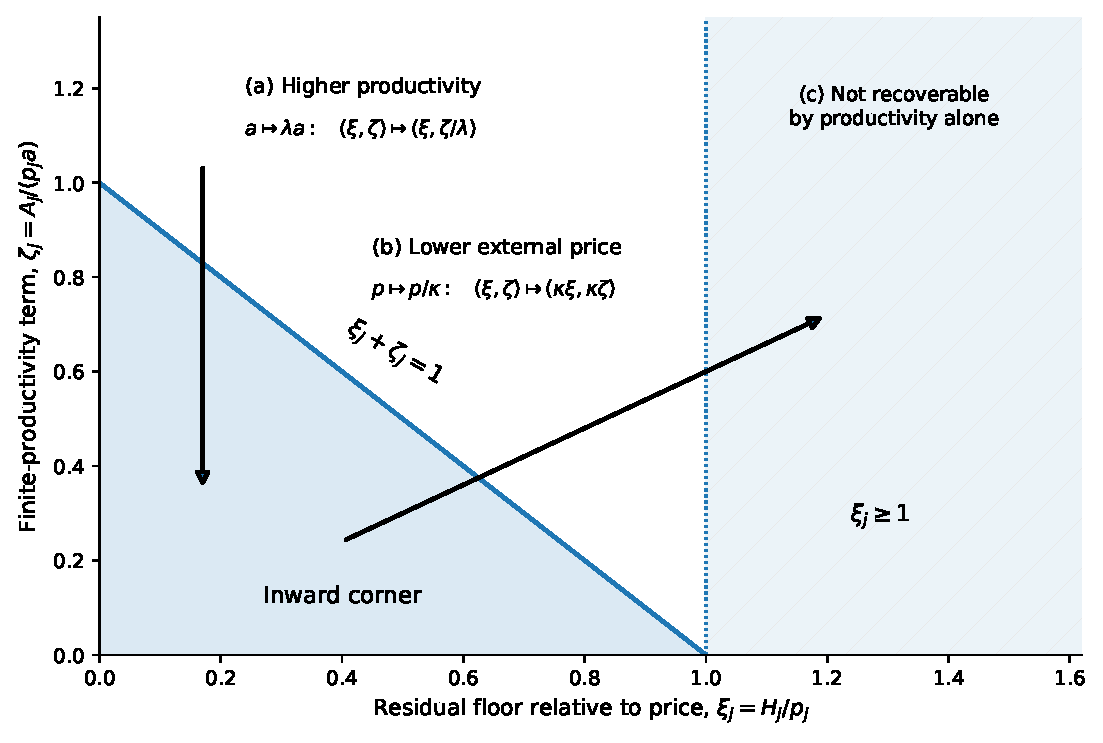
\includegraphics[width=.91\textwidth]{fig3.pdf}
\caption{Exact logarithmic phase diagram and comparative statics for one
external direction. The shaded triangle satisfies
$H_j/p_j+A_j/(p_ja)\leq1$; every external direction must satisfy this
condition for the all-inward corner to be optimal.
(a) Higher productivity reduces only $\zeta_j$, producing a downward
vertical move. (b) A price reduction to $p_j/\kappa$ multiplies both
coordinates by $\kappa$, producing a radial move away from the origin.
(c) In the hatched region $\xi_j\geq1$, no finite productivity restores
the corner. For $A_j>0$, $(1,0)$ is only a limiting point.
The arrows are schematic evaluations of the exact transformations;
no archived inputs are overlaid and no population frequency is estimated.}
\label{fig:phase}
\end{figure}


\begin{samepage}
\subsection{Shared technological change}
\begin{corollary}[Shared gains and the phase coordinates]
\label{cor:shared-technology}
Fix $B,d_0,S_j$ and logarithmic local production and value. Under
$(a,r_j,p_j)\mapsto(\lambda_a a,\lambda_r r_j,p_j/\kappa)$, with
$\lambda_a,\lambda_r,\kappa>0$, \cref{eq:HA,eq:phase-coordinates} give
\begin{equation}
 \xi'_j=\kappa\xi_j,\qquad
 \zeta'_j=\frac{\kappa}{\lambda_a}
 \left[\zeta_j+\frac{(1+B)(\lambda_r-1)r_j}{p_ja}\right].
 \label{eq:shared-technology}
\end{equation}
\end{corollary}
\end{samepage}
The identity also covers zero slopes; see \cref{app:shared-technology-proof}.
Cheaper external projects enlarge the productivity-independent floor.
Productivity cannot offset this increase in $\xi_j$.
Manufacturing improvements affecting both local substrates and replicating
platforms therefore do not guarantee inwardness; no particular implementation
is assumed. The archived Table~\ref{tab:scenarios} illustrates the distinction:
local productivity multiplied by ten changes 219 inward cases to 314;
shared productivity gives 222; the external price-floor factor $0.01$ gives zero.

\section{Persistence: growing versus bounded budgets}
\label{sec:persistence}

\subsection{Unbounded physical budgets}

\begin{proposition}[Growth obstruction and sharp productivity scaling]
\label{prop:growth-trichotomy}
Let $B(t)\to\infty$, let $\ell$ be concave, and retain the assumptions
of \cref{prop:hub}. Suppose that eventually some direction has
$p_j(t)\leq M<\infty$ and $S_j(t)\geq s>0$.
For $\eta\geq1$, the all-inward corner is excluded at every sufficiently
late time, for every path of finite positive productivities $a(t)$.
For $0\leq\eta<1$, eventual inwardness instead requires
\begin{equation}
 \Omega(t)\geq
 \left[\frac{s\Gamma(B(t))}{M}\right]^{1/(1-\eta)}
 \geq\left[\frac{sB(t)}{M}\right]^{1/(1-\eta)}.
 \label{eq:necessary-output-growth}
\end{equation}
For the sufficiency statement, additionally fix all $p_j>0$, finite
$r_j,S_j\geq0$, and $d_0$. If $0<\eta<1$, it is sufficient that,
eventually,
\begin{equation}
 \Omega(t)\geq c_\Omega\Gamma(B(t))^{1/(1-\eta)},\qquad
 c_\Omega>
 \left(\max_j\frac{S_j}{p_j}\right)^{1/(1-\eta)}.
 \label{eq:sufficient-output-growth}
\end{equation}
The inequalities then become strict. For $\eta=0$, the exact condition is
\begin{equation}
 \frac{\Omega(t)}{\Gamma(B(t))}=a(t)\ell'(B(t))
 \geq\max_j\frac{r_j+S_j}{p_j}.
 \label{eq:linear-value-growth}
\end{equation}
In particular, for $\ell(z)=z$ and $0<\eta<1$,
$a(t)\geq c_\Omega B(t)^{\eta/(1-\eta)}$ with the strict coefficient
condition above is eventually sufficient.
\end{proposition}
\noindent\emph{Proof sketch.}
For $\eta=1$ the residual term has positive infimum one after division
by $S_j\Gamma$. For $\eta>1$ that infimum is
\begin{equation}
 \min_{\Omega>0}\frac{(d_0+\Omega)^\eta}{\Omega}
 =d_0^{\eta-1}\frac{\eta^\eta}{(\eta-1)^{\eta-1}}.
 \label{eq:residual-minimum}
\end{equation}
Both conflict with $\Gamma(B)\geq B\to\infty$. Below unit curvature,
comparison with $\Omega^{\eta-1}$ gives the necessary rate; the strict
coefficient in \cref{eq:sufficient-output-growth} leaves an asymptotic
margin for remote computational returns. See \cref{app:growth-proof}.

\paragraph{Remark (Bounded productivity on growing budgets).}
Under \cref{prop:growth-trichotomy}, $a\leq a_{\max}<\infty$ gives
$\Omega=O(B)$ by concavity. For $0<\eta<1$, this contradicts
\cref{eq:necessary-output-growth}; an eventually inward path requires
$a(t)\to\infty$. At $\eta=0$, \cref{eq:linear-value-growth} still uses
actual productivity; its necessary ceiling test is
$a_{\max}\ell'(B(t))\geq\max_j(r_j+S_j)/p_j$.
A positive right-hand side and vanishing local marginal production
therefore exclude persistence. See \cref{app:ceiling-growth-proof}.

This result concerns the growth of physical resources, not the growth
of computational efficiency. With persistent residual value and bounded
prices, productivity can compensate for an unbounded resource budget
only on the $\eta<1$ branch of the concave-production model. The endpoint
$\eta=0$ must retain $r_j$ as well as $S_j$; remote computation is not a
vanishing correction in that case.

\begin{corollary}[Logarithmic pathwise specialization]
\label{prop:persistence}
Let $\ell(z)=\ln(1+z)$ and $\eta=1$, with fixed $r_j,d_0$ and finite
positive $B(t),a(t),p_j(t)$. Define $H_j(t),A_j(t)$ by
\cref{eq:HA}. On any specified path, the corner is optimal at every
time exactly when, in every direction with $A_j(t)>0$,
\begin{equation}
 p_j(t)>H_j(t),\qquad
 a(t)\geq\max_{j:A_j(t)>0}
       \frac{A_j(t)}{p_j(t)-H_j(t)}.
 \label{eq:pathwise}
\end{equation}
In particular, where $S_j(t)>0$,
\begin{equation}
 \frac{p_j(t)}{S_j(t)}>[1+B(t)]\ln[1+B(t)].
 \label{eq:path-ratio}
\end{equation}
For $B(t)\to\infty$, fixed positive residual slopes therefore require
prices at least of order $B\ln B$; bounded prices require
$S_j(t)=O((B\ln B)^{-1})$. These rate restrictions do not replace the
productivity inequality. A zero-slope direction with $r_j>0$ requires
$a(t)\geq[1+B(t)]r_j/p_j(t)$.
\end{corollary}
\begin{proof}
Apply \cref{eq:exact,eq:acrit} at each time. Non-negativity and $d_0>0$
imply $A_j=0$ exactly when $r_j=S_j=0$. Division by a positive slope
and $(1+B)\ln(1+B)\sim B\ln B$ give the rate statements.
\end{proof}


\subsection{What increasing returns would have to accomplish}

\begin{proposition}[At least exponential local returns]
\label{prop:exponential-necessity}
Let $\eta=1$ and retain the model assumptions apart from local
concavity. Let a fixed local production function satisfy $\ell(0)=0$
and be continuously differentiable and positive with positive derivative
for positive budgets. Let $B(t)$ be continuous with $B(t)\to\infty$.
If eventually $p_j(t)\leq M$, $S_j(t)\geq s>0$, and the corner is
optimal at every time, then for all sufficiently large $B$,
\begin{equation}
 \frac{\dd\ln\ell(B)}{\dd B}>\frac{s}{M},\qquad
 \ell(B)>\ell(B_0)\exp\!\left[\frac{s}{M}(B-B_0)\right]
 \quad(B>B_0).
 \label{eq:exponential-necessity}
\end{equation}
Convex local production gives $\Gamma(B)\leq B$, but polynomial
superlinearity is insufficient: $\ell(z)=z^k$ gives $\Gamma=B/k$.
By contrast, $\ell(z)=[\exp(\psi z)-1]/\psi$, $\psi>0$, gives
$\Gamma=[1-\exp(-\psi B)]/\psi<1/\psi$.
\end{proposition}
\noindent\emph{Proof sketch.}
The necessary strict floor gives $\ell'/\ell>S_j/p_j\geq s/M$.
Continuity of the budget path covers every sufficiently large budget,
so integration proves the exponential bound. The remaining identities
follow by differentiation; see \cref{app:returns-proof}.

The required increase is with local resource investment, not merely
with calendar time. This supplies a quantitative test for
compression-based inward development proposals such as
\citet{Smart2012}. Increasing returns remove the concavity guarantee.
For exponential local production with one affine external channel and
linear residual value, an exact global test is available: the corner
must satisfy its first-order condition and outperform the all-external
endpoint (\cref{lem:exponential-endpoints}). Smooth concave residual
utilities, or smooth concave external production, can invalidate this
two-test shortcut. Explicit counterexamples are given in
\cref{app:exponential-counterexamples}.

\subsection{The tipping budget}

\begin{proposition}[A unique productivity-independent tipping budget]
\label{prop:tipping}
Let $\eta=1$ and $\ell\in C^2([0,\infty))$, with $\ell(0)=0$,
$\ell'>0$, and $\ell''\leq0$. Fix $d_0\geq1$, all $p_j>0$, and finite
$r_j,S_j\geq0$. If at least one $S_j>0$, define $B_{\rm tip}$ by
\begin{equation}
 \Gamma(B_{\rm tip})=\min_{j:S_j>0}\frac{p_j}{S_j}.
 \label{eq:tipping-budget}
\end{equation}
This budget exists and is unique, since
\begin{equation}
 \Gamma(0)=0,\qquad
 \Gamma'(B)=1-\frac{\ell(B)\ell''(B)}{\ell'(B)^2}\geq1.
 \label{eq:gamma-monotone}
\end{equation}
The corner is attainable at finite productivity exactly for
$0<B<B_{\rm tip}$, where its threshold is
$a_{\rm crit}^{\ell}(B)$ from \cref{eq:acrit-general}.
This threshold is non-decreasing and diverges as
$B\uparrow B_{\rm tip}$. At $B=B_{\rm tip}$ as well as above it,
no finite productivity makes the corner optimal.
If eventually $B(t)\leq B'<B_{\rm tip}$ and
$a(t)>a_{\rm crit}^{\ell}(B')$, every static optimizer is eventually
all-inward. If every $S_j=0$, set
$B_{\rm tip}=\infty$; no finite productivity-independent residual
barrier exists.
\end{proposition}
\noindent\emph{Proof sketch.}
Differentiate $\Gamma$. Below its unique crossing, every denominator
in \cref{eq:acrit-general} is positive. Each nontrivial threshold is
non-decreasing because its denominator has derivative
$p_j\ell''-S_j\ell'\leq0$. A binding positive-slope denominator
vanishes at the crossing. See \cref{app:tipping-proof}.

\begin{corollary}[The effective budget under a productivity ceiling]
\label{cor:ceiling-budget}
Retain \cref{prop:tipping} with some $S_j>0$ and fix
$0<a_{\max}<\infty$. Define
\begin{equation}
 B^*(a_{\max})=\sup\{B\in(0,B_{\rm tip}):
                     a_{\rm crit}^{\ell}(B)\leq a_{\max}\},
 \qquad \sup\varnothing:=0.
 \label{eq:ceiling-budget}
\end{equation}
An inward optimum at some $0<a\leq a_{\max}$ exists exactly for
$0<B\leq B^*(a_{\max})$. If $B^*>0$, its endpoint is included and
$a_{\rm crit}^{\ell}(B^*)=a_{\max}$; an actual productivity must still
meet \cref{eq:acrit-general}. Moreover, $B^*<B_{\rm tip}$,
$B^*$ is non-decreasing in $a_{\max}$, and $B^*\to B_{\rm tip}$ as
$a_{\max}\to\infty$.
\end{corollary}
An efficiency redesign can raise this effective budget, but never beyond
$B_{\rm tip}\leq\min_{j:S_j>0}p_j/S_j$, since $\Gamma(B)\geq B$.
The empty-set and equality cases are proved in \cref{app:ceiling-budget-proof}.

\begin{corollary}[Fixed- and bounded-budget curvature]
\label{prop:curvature}
At a fixed positive budget and under concave production, each nontrivial
direction has a unique finite high-productivity threshold for
$0\leq\eta<1$. At $\eta=1$, \cref{eq:acrit-general} applies.
At $\eta>1$, a direction with $S_j>0$ has an inward set in $a>0$
that is empty, a singleton, or a bounded closed interval. A direction
with $S_j=0$ requires only $a\geq r_j/[p_j\ell'(B)]$ for every $\eta$.
For the local logarithm the test is precisely
\begin{equation}
 r_j+S_j(d_0+aL)^\eta\leq\frac{p_ja}{1+B},
 \qquad L=\ln(1+B).
 \label{eq:iso-corner}
\end{equation}
For the path statements fix the parameters and assume $\ell$ is $C^1$
with positive derivative near $B(t)\to\bar B\in(0,\infty)$.
For $\eta<1$, eventually exceeding a sufficiently large finite productivity
threshold gives eventual strict inwardness. This also holds for any
$0<B(t)\leq B_{\max}<\infty$ under concavity and
$\ell'(B_{\max})>0$. For $\eta>1$ and some $S_j>0$, eventually
exceeding a sufficiently large finite threshold instead excludes inwardness
near the positive limit. At $\eta=1$, $\bar B<B'<B_{\rm tip}$ and
eventual $a(t)>a_{\rm crit}^{\ell}(B')$ suffice; $\bar B>B_{\rm tip}$
excludes inwardness. At equality the pointwise comparison with
$a_{\rm crit}^{\ell}(B(t))$ remains indispensable.
\end{corollary}
\noindent\emph{Proof.}
See \cref{app:curvature-proof}. This is the fixed-budget curvature
classification, with a uniform bound near the positive limiting budget;
it is not a new assumption about preferences. ``No tipping budget''
for $\eta<1$ means no productivity-independent finite obstruction,
not absence of a budget threshold at a fixed productivity.

For $\eta>1$, computational value saturates while residual motives persist:
sufficiently large efficiency gains reduce the marginal value of local
investment and eventually favour an external deviation, not permanent inwardness.

\subsection{Resource acquisition and the inward basin}

Separate resources available locally from those supplied by prior
replicating acquisition. In discrete planning periods, write
\begin{equation}
 B_t=B_{\rm loc}(t)+g_XX_t,\qquad
 X_{t+1}=X_t+x_t,\qquad g_X\geq0,
 \label{eq:acquisition-stock}
\end{equation}
where $B_{\rm loc}(t)$ is non-decreasing with limit $\bar B>0$.
Only the replicating channel enters $X$; observation alone does not.
With no previous acquisition, an all-inward history has $X=0$ and
$B_t\leq\bar B$. Stopping new investment later does not erase an
inherited external stock. Since both stock and local mobilization are
non-decreasing, a crossing of $B_{\rm tip}$ cannot be reversed in this
model. In a multi-channel model this excludes all-inward expenditure,
not necessarily zero replication.

A basin cannot be specified by four scalar parameters without also
specifying the resource-mobilization path and the full residual utility.
The following benchmark fixes both. It uses one replicating channel,
linear residual value, and an already mobilized local ceiling.

\begin{proposition}[A unique inward-basin boundary]
\label{prop:basin}
Fix $p>0$, $S>0$, $r\geq0$, $d_0\geq1$, $g_a>0$, and $g_X>0$.
Let $X_0=0$, $B_{\rm loc}(t)=\bar B$, $a_t=a_0\exp(g_at)$, and
$0<\bar B<B_{\rm tip}$, where
$(1+B_{\rm tip})\ln(1+B_{\rm tip})=p/S$.
At each period choose the unique maximizer
\begin{equation}
 x^*(B,a)=\underset{0\leq x\leq B/p}{\arg\max}
 \left\{\ln[d_0+a\ln(1+B-px)+rx]+Sx\right\}.
 \label{eq:basin-policy}
\end{equation}
There is a unique
$a_{\rm sep}(g_a,g_X,\bar B)\in(0,a_{\rm crit}^{\ell}(\bar B))$
with the following classification:
\begin{itemize}[leftmargin=*,nosep]
\item If $a_0>a_{\rm sep}$, new external investment stops in finite time
and stays zero, at a budget strictly below $B_{\rm tip}$.
\item If $a_0<a_{\rm sep}$, the budget reaches or exceeds $B_{\rm tip}$
in finite time and new external investment remains positive thereafter.
\item If $a_0=a_{\rm sep}$, every finite-time investment is positive,
but $B_t\uparrow B_{\rm tip}$ and
$g_X\sum_{t\geq0}x_t=B_{\rm tip}-\bar B$.
\end{itemize}
Whenever $B_t\geq B_{\rm tip}$,
\begin{equation}
 x_t>\frac{B_t-B_{\rm tip}}p,\qquad
 B_{t+1}-B_{\rm tip}>
 (1+g_X/p)(B_t-B_{\rm tip}).
 \label{eq:runaway-bound}
\end{equation}
The boundary $a_{\rm sep}$ is non-increasing in $g_a$ and
non-decreasing in $g_X$ and in $\bar B/B_{\rm tip}$, with the other
parameters fixed.
\end{proposition}
\noindent\emph{Proof sketch.}
The unique static investment is continuous, increases with the budget,
and decreases with productivity. A path that neither stops nor crosses
must converge to the tipping budget. Two such paths cannot coexist:
a positive gap between their budgets cannot shrink. Continuity separates
the open sets of stopping and crossing paths, giving exactly one boundary.
The complete proof and finite-time basin certificates are in
\cref{app:basin-proof}.

\begin{corollary}[Saturating productivity and the inward basin]
\label{cor:capped-basin}
Retain the one-channel model and parameter assumptions of \cref{prop:basin},
but replace its productivity path.
(i) If $a_t$ is positive, non-decreasing, and bounded by
$a_{\max}<a_{\rm crit}^{\ell}(\bar B)$, every path reaches
$B_{\rm tip}$ in finite time.
(ii) Let
\begin{equation}
 a_t=a_{\max}-(a_{\max}-a_0)\exp(-g_at),\quad
 0<a_0\leq a_{\max},\quad a_{\max}>a_{\rm crit}^{\ell}(\bar B).
 \label{eq:saturating-productivity}
\end{equation}
If some initial productivity crosses $B_{\rm tip}$, a unique
$a_{\rm sep}\in(0,a_{\rm crit}^{\ell}(\bar B))$ separates finite-time
capture at higher initial productivity from crossing at lower productivity.
Its boundary path has $x_t>0$ and
$B_t\uparrow B^*(a_{\max})$, not $B_{\rm tip}$.
After reaching $B_{\rm tip}$, \cref{eq:runaway-bound} applies in both cases.
\end{corollary}
The crossing hypothesis is essential: all paths can instead be captured.
The proof and a hard-cap counterexample to the uncaptured-boundary
classification are in \cref{app:capped-basin-proof}.

For example, let $(p,S,r,d_0)=(1,0.002,0.05,1)$,
$g_a=0.05$, $g_X=0.5$, and $\bar B=0.6B_{\rm tip}$. New calculations
give $B_{\rm tip}=106.001289$,
$a_{\rm crit}^{\ell}(\bar B)=7.279612$, and
$a_{\rm sep}\simeq6.63216$. Starting at $a_0=0.5$ crosses the tipping
budget at $t=2$; starting at $a_0=50$ is inward from the start. With
$a_0=0.5$ but $g_X=0$, investment stops at $t=54$, not at $t=0$.
Thus removing resource feedback removes this lock-in mechanism, not
the initial incentive to expand.

Lock-in here names an absorbing allocation regime, not a welfare
mistake. Additional resources do not reduce the feasible set. In this
costless, non-depreciating stock benchmark, any finite-horizon
continuation value is non-decreasing in $X$: this follows by backward
induction because a larger stock permits the same current project and
more local investment. A strictly improving myopic external deviation
therefore remains improving after adding such a continuation. A
forward-looking planner need not avoid the tipping budget. Productive
local alternatives require the separate dynamic comparison developed
in the infinite-horizon subsection.

\paragraph{Speculative physical mapping (conjecture).}
If a fixed-horizon energy budget increases with usable host luminosity,
and if denser stellar neighbourhoods reduce external resource prices
while leaving residual values fixed, both changes raise
$\bar B/B_{\rm tip}$. The basin comparison then suggests a greater
propensity to expand. The conjecture concerns these physical parameter
mappings, not the proved comparative static. With bounded efficiency,
\cref{cor:capped-basin} adds the effective ceiling and crossing qualification.

\subsection{An infinite-horizon benchmark}
\label{sec:dynamic}
Myopic resource acquisition and optimal intertemporal allocation answer
different questions. To obtain a transparent infinite-horizon benchmark,
replace logarithmic production by linear production, omit the additive
computational baseline, and use logarithmic value of strictly positive
computation. Let
\begin{equation}
 z_t+px_t=B_t,\quad C_t=a_Lz_t+a_Xx_t,\quad
 B_{t+1}=g_Lz_t+g_Xx_t,\quad
 \max\sum_{t=0}^{\infty}\beta^t\ln C_t.
 \label{eq:infinite-model}
\end{equation}
Here $B_0,p,a_L,a_X,g_L,g_X>0$ and $0<\beta<1$.
All these parameters are constant. This benchmark is homothetic; it is
not the previous logarithmic production model under different notation.
For $s=px/B$, define
$A(s)=a_L(1-s)+(a_X/p)s$ and
$G(s)=g_L(1-s)+(g_X/p)s$.

\begin{proposition}[Infinite-horizon verification and the inward policy]
\label{prop:infinite}
Every feasible policy has absolutely convergent discounted log returns.
Writing
\begin{equation}
 H_\beta(s)=(1-\beta)\ln A(s)+\beta\ln G(s),\qquad
 H_\beta^*=\max_{0\leq s\leq1}H_\beta(s),
 \label{eq:homothetic-index}
\end{equation}
the value function is
\begin{equation}
 V(B)=\frac{\ln B}{1-\beta}
       +\frac{H_\beta^*}{(1-\beta)^2}.
 \label{eq:infinite-value}
\end{equation}
A constant maximizing share is optimal forever. The all-inward policy
is optimal if and only if
\begin{equation}
 (1-\beta)\frac{a_X/p}{a_L}
       +\beta\frac{g_X/p}{g_L}\leq1.
 \label{eq:infinite-inward}
\end{equation}
For every feasible path, $\beta^T V(B_T)\to0$; this transversality
condition validates the Bellman telescoping argument despite unbounded
logarithmic returns.
\end{proposition}
\noindent\emph{Proof sketch.}
Positive production and growth endpoints bound $|\ln B_t|$ by a linear
function of $t$. Discounting therefore controls both tails. Substitution
of \cref{eq:infinite-value} into the Bellman equation leaves the one-share
maximization in \cref{eq:homothetic-index}; its derivative at zero gives
\cref{eq:infinite-inward}. The complete verification is in
\cref{app:infinite-proof}. The argument supplies its own growth bounds,
rather than invoking a bounded-reward contraction. It is consistent with
the homogeneous-function approach of \citet{AlvarezStokey1998}.

\begin{corollary}[Static reversals and the patient limit]
\label{cor:infinite-reversals}
Static inwardness is neither necessary nor sufficient for infinite-horizon
inwardness. If $(g_X/p)/g_L<1$, sufficiently patient planners are inward;
if this ratio is greater than one, they are not. At equality, the current
computational-return ratio still decides for every $\beta<1$.
\end{corollary}
\begin{proof}
With $\beta=0.9$, return ratios $(0.5,2)$ give a weighted ratio $1.85$:
static inwardness fails dynamically. Ratios $(2,0.5)$ give $0.65$:
static outwardness reverses. Taking $\beta\uparrow1$ proves the two
strict growth cases. With equal growth ratios, subtracting one leaves
$(1-\beta)[(a_X/p)/a_L-1]$, proving the equality case.
\end{proof}

The same derivative decomposition contains the earlier two-period
examples, although their nonlinear production is not a literal special
case of \cref{eq:infinite-model}. For a concave differentiable first-period
objective $U_1(x)$ and increasing concave continuation $V_2$, the following
short transfer result supplies that exact nesting.
\begin{corollary}[A future-adjusted inward condition]
\label{prop:dynamic}
If $W(x)=U_1(x)+\beta V_2(B_{20}+g_LB_1+(g_X-p_1g_L)x)$
is defined on $[0,B_1/p_1]$, it is concave and its inward endpoint is
optimal exactly when
$U_1'(0)+\beta V_2'(B_{20}+g_LB_1)(g_X-p_1g_L)\leq0$.
\end{corollary}
\begin{proof}
Composition with the affine continuation budget preserves concavity.
The right derivative at the endpoint has the displayed value, and a
concave differentiable function has its maximum there exactly when this
derivative is non-positive. Substituting the archived $U_1,V_2$ yields
\cref{eq:dynamiccriterion} in the supplement.
\end{proof}
The archived threshold $g_X=\DynamicThreshold$ and allocation
$x=\DynamicOutward$ remain unchanged. Their full construction and
\cref{fig:dynamic} are supplementary evidence for these reversals.

\subsection{Residual value and a local ceiling break homotheticity}
Adding $Sx_t$ with $S>0$ makes the reward scale with $B_t$, whereas the
logarithmic reward changes only additively under resource scaling. The
closed form \cref{eq:infinite-value} then ceases to apply. A sufficient
condition for finite values is
$\beta\max(g_L,g_X/p)<1$. If $\beta g_X/p\geq1$, perpetual
all-external investment already has infinite positive residual value;
it cannot be used as a finite-value optimization counterexample.

\begin{corollary}[An unbounded-budget obstruction survives foresight]
\label{cor:dynamic-residual}
In the finite-value residual model, an all-inward infinite-horizon policy
can be optimal from a state $B$ only if
\begin{equation}
 \frac{SB}{p}\leq
 \frac{1-(1-\beta)(a_X/p)/a_L-\beta(g_X/p)/g_L}{1-\beta}.
 \label{eq:dynamic-residual-floor}
\end{equation}
Thus such a policy cannot persist along $B_t\to\infty$ with constant
positive $S$ and fixed finite coefficients.
\end{corollary}
\noindent\emph{Proof sketch.}
Deviate once and then follow the all-inward policy. The continuation log
value has derivative $1/[(1-\beta)B]$. Its contribution plus the current
residual derivative gives \cref{eq:dynamic-residual-floor}; see
\cref{app:infinite-proof}. This is a necessary policy test, not a complete
solution to the nonhomothetic Bellman equation. At $\beta=0$ it is the
linear-production logarithmic floor without a shifted baseline.

An explicit local ceiling can instead enter through
\begin{equation}
 B_{t+1}=\min\{\bar B,g_L(B_t-px_t)\}+g_Xx_t.
 \label{eq:capped-transition}
\end{equation}
Along an all-inward path this keeps future budgets below $\bar B$.
The transition is no longer homogeneous. For the shifted-log production
and linear-residual model of \cref{prop:tipping}, suppose a finite
increasing continuation value exists and $g_X\geq pg_L$. Then a small
external deviation never reduces next-period resources. Consequently,
at $B\geq B_{\rm tip}$ the strictly positive current external derivative
cannot be reversed by continuation value. Below the tipping budget,
future resource acquisition can still overturn the static inward optimum.
A direct one-step proof is given in \cref{app:infinite-proof}.
This is the valid connection between the local ceiling and the tipping
budget; it does not impose the static basin separator on a forward-looking
planner.

\section{Which residual value survives}
\label{sec:residual}

The all-inward corner is a stringent diagnostic, but it is not the correct
boundary for a claim about the absence of new replicating lineages.
Information can be purchased without resident settlement. A dormant,
externally stored backup can provide geographical separation without
continuing resource acquisition. This section first prices those substitutes
and then replaces a free resilience slope by an explicit expected-value
calculation. The resulting distinctions identify which part of the earlier
floor is a replication incentive rather than merely an external-service
incentive.

\subsection{No replication with observation and dormant backups}
Add an optional dormant-backup capacity $b_{\rm bk}\geq0$ at price $p_b>0$.
It has neither computational production nor descendants. The budget and
objective become
\begin{align}
 z+p_nx+p_hy+p_mw+p_bb_{\rm bk}&\leq B,\nonumber\\
 U&=F(C)+(1-q)E(x)+\epsilon_RR(x+y+b_{\rm bk})
                  +\epsilon_II(x+y+w).
 \label{eq:backup-model}
\end{align}
Throughout this subsection local production is concave; all other functions retain the concavity assumptions of \cref{sec:allocation}.
The no-replication face has $x=y=0$; observation and backups are optimized,
not fixed at zero. Write a maximizing allocation on this face as
$(z^*,w^*,b^*)$, its computation as $C^*$, and its budget multiplier as
$\lambda>0$. Assume derivatives are finite at this allocation. If $z^*>0$,
then $\lambda=F'(C^*)a\ell'(z^*)$. With $z^*=0$, the multiplier, rather
than an unjustified interior formula, is used below.

\begin{proposition}[A no-replication criterion]
\label{prop:no-replication}
A no-replication face optimizer is also a global optimizer exactly when
it admits a restricted-problem multiplier $\lambda$ satisfying
\begin{align}
 F'(C^*)r_n+(1-q)E'(0)+\epsilon_RR'(b^*)+\epsilon_II'(w^*)
     &\leq p_n\lambda,\nonumber\\
 F'(C^*)r_h+\epsilon_RR'(b^*)+\epsilon_II'(w^*)
     &\leq p_h\lambda.
 \label{eq:no-replication}
\end{align}
The non-replicating channels satisfy
$\epsilon_II'(w^*)\leq p_m\lambda$ and
$\epsilon_RR'(b^*)\leq p_b\lambda$, with equality in each positive
channel. The backup inequality is omitted when backups are unavailable.
Strict inequalities in \cref{eq:no-replication} exclude replication in
every full optimizer.
\end{proposition}
\noindent\emph{Proof sketch.}
The restricted first-order conditions already control the local,
observation, and backup directions. Adding the two displayed inequalities
completes the full concave-program optimality conditions. A supporting
hyperplane proves global sufficiency. The converse and endpoint cases
are proved in \cref{app:replication-proof}.

When observation is interior and backups are absent, this gives exactly
\begin{align}
 F'(C^*)r_n+(1-q)E'(0)+\epsilon_RR'(0)&\leq(p_n-p_m)\lambda,\nonumber\\
 F'(C^*)r_h+\epsilon_RR'(0)&\leq(p_h-p_m)\lambda.
 \label{eq:observation-net}
\end{align}
Information disappears as a separate replication premium, not as an
economic influence: it still determines $w^*$, the remaining local
investment, and $\lambda$. For an interior backup but a possibly inactive
observation channel, the corresponding subtraction is $p_b\lambda$, while
$\epsilon_II'(w^*)$ stays explicit. If both are interior, the comparison
uses the net bundle prices $p_j-p_m-p_b$.

\begin{corollary}[Substitute bundles and zero-service corners]
\label{cor:bundle}
At a no-replication face optimum with $w^*,b^*>0$, $p_h<p_m+p_b$
rules out no replication even if $r_h=0$. At equality with $r_h=0$,
replacing equal small amounts of observation and backup by industry
preserves value and expenditure, and can produce tied replicating optima.
If $w^*=0$, the correct reduction instead uses
$c_I=\epsilon_II'(0)/\lambda\leq p_m$; it does not subtract the full
observation price. Analogously an inactive backup uses
$c_R=\epsilon_RR'(0)/\lambda\leq p_b$.
\end{corollary}
\noindent\emph{Proof sketch.}
Use complementary slackness in \cref{eq:no-replication}. A cheaper bundle
has a strictly positive replication derivative. The exact exchange and
zero-channel cases are established in \cref{app:replication-proof}.

The bundle result is important for interpreting inexpensive autonomous
industry. Replacing colonists by observation instruments does not help
if a replicating industrial platform supplies both observation and
resilience more cheaply than their standalone substitutes. Conversely,
expensive industrial platforms can lose even when information and
resilience have positive value. The model consequently does not need
to erase those motives; it needs a technologically credible way to meet
them without a reproducing platform. Independence from a particular
service premium is not independence from the prices of its substitutes.

The distinction between exactly zero and a small positive launch rate
is consequential only with a propagation mechanism. A deployed viable
seed in a deterministic growth law $N(t)=N(0)\exp(g t)$ with $g>0$ never
becomes equivalent to $N(0)=0$. A stochastic supercritical lineage instead
has a positive survival probability, not guaranteed survival. Finite
launch sizes, deployment thresholds, and subcritical replication do not
justify the stronger claim that every arbitrarily small investment expands
without bound. The population calculation in \cref{sec:population} uses
successful, arriving fronts rather than an investment share as its unit.


\subsection{A constructive separation from all-inward persistence}
The distinction above can change the asymptotic conclusion, not just a
finite-budget classification. In the following construction, physical
budgets are supplied exogenously to the sequence of static problems.
The proposition does not specify how those resources are acquired.

\begin{corollary}[Growing budgets without new replication]
\label{cor:growing-no-replication}
Let $\eta=1$, $B\to\infty$, $a=B^2$, $q=1$, $C_0\geq0$, and
$\ell(z)=\ln(1+z)$. Let
$\epsilon_I I(w)=J_I[1-\exp(-w/s_I)]$ and
$\epsilon_R R(b)=J_R[1-\exp(-b/s_R)]$, with fixed strictly positive
$J_I,J_R,s_I,s_R,p_m,p_b$. External computation is concave with fixed
finite initial slopes. If $p_n,p_h>p_m+p_b$, then for all sufficiently
large $B$ every full optimizer has $x=y=0$, and a no-replication optimizer
has $w,b>0$ with
\[
 z/B\longrightarrow1,\qquad w+b=O(\ln B).
\]
Nevertheless the all-inward corner is eventually impossible because its
information and resilience slopes stay positive.
\end{corollary}
\noindent\emph{Proof sketch.}
The restricted face has positive local investment for large $B$.
Its local multiplier tends to zero, making both service channels interior.
Their exponential marginal utilities give service quantities logarithmic
in the inverse multiplier, hence $B=z+O(\ln z)$. The remaining replication
premium divided by that multiplier is $r_j(1+z)/B^2\to0$, smaller than
either strictly positive net price. A complete proof is in
\cref{app:growing-norep-proof}.

\paragraph{Remark (The growth construction uses $a=B^2$).}
Keep the other assumptions of \cref{cor:growing-no-replication}, but
impose $0<a\leq a_{\max}<\infty$. Then $F'(C^*)/\lambda\to\infty$,
so every channel with $r_j>0$ eventually violates
\cref{eq:replication-reduced}. At $z^*>0$ this ratio is $(1+z^*)/a$.
With both services interior and $\Delta_j=p_j-p_m-p_b>0$, the exact test is
$a\ell'(z^*)\geq r_j/\Delta_j$; its ceiling counterpart
$a_{\max}\ell'(z^*)\geq r_j/\Delta_j$ is necessary, not sufficient.
For $r_j=0$ the channel passes automatically. The proof, including $z^*=0$,
is in \cref{app:norep-ceiling-proof}. This is the same declining-marginal-production
budget effect isolated by \cref{eq:budgetcrit}.

This construction is a counterexample to transferring the all-inward
unbounded-budget exclusion directly to no replication. Non-replicating
services absorb a persistent preference rather than requiring its weight
to vanish. It also explains why a local ceiling below the original
$B_{\rm tip}$ cannot be a universal necessary condition once the decision
problem changes. The relevant comparison uses the remaining local budget,
the optimized shadow value of resources, and the net service-bundle price.
A physical application must still provide a feasible resource history;
the construction is a separation of allocation claims, not a mechanism
for obtaining unbounded local energy.

The price condition is strict for a reason. If an industrial project
costs exactly the sum of its substitute services and has no computational
return, the exchange in \cref{cor:bundle} can leave a continuum of tied
choices. An analyst selecting the non-replicating member of that set has
shown existence, not suppression of every replicating choice. Conversely,
if industry costs less than the bundle, improving local computation cannot
repair the negative net price while both substitutes remain interior.
This distinction matters at the population step: a positive measure of
ties resolved outward can create arrival exposure even where an inward
optimizer exists. Strict preference, an explicit tie-breaking rule, or a
separate containment constraint is needed to exclude that route.

\subsection{Value at risk rather than an exogenous resilience slope}
For a precise local calculation, specialize to one candidate backup
project $x$, $C(x)=a\ell(B-px)+G(x)$, $G'(0)=r$, and $C(0)=\Omega>0$.
Set $C_0=0$ in this calculation. Let $0\leq\vartheta<1$ be the
probability, over the stated horizon, of a catastrophe that separation
can mitigate. It is not a rate in inverse years. Let $\varphi(0)=0$,
$0\leq\varphi\leq1$, and $\varphi'(0)>0$. A seed backup has
$\gamma=0$; a scale-matched mirror has $\gamma=1$. Use
\begin{equation}
 U_R(x)=\left[1-\vartheta+\vartheta
       \varphi\!\left(\frac{x}{C(x)^\gamma}\right)\right]F_\eta(C(x)).
 \label{eq:risk-utility}
\end{equation}
This specifies both the value at risk and the probability of retaining it.
Its product form need not be concave.

\begin{proposition}[The endogenous-risk floor]
\label{prop:endogenous-risk}
Assume a feasible right neighbourhood of $x=0$ has $C(x)>0$ and all
functions in \cref{eq:risk-utility} are differentiable there. A necessary
condition for $x=0$ to maximize $U_R$ is
\begin{equation}
 p\geq\frac{\Gamma r}{\Omega}
 +\frac{\vartheta}{1-\vartheta}\varphi'(0)
       \Gamma\Omega^{-\gamma}K_\eta(\Omega),\qquad
 K_\eta(\Omega)=\frac{F_\eta(\Omega)(1+\Omega)^\eta}{\Omega}.
 \label{eq:risk-floor}
\end{equation}
For $0\leq\eta<1$, $K_\eta(\Omega)\to(1-\eta)^{-1}$ as
$\Omega\to\infty$. For $\eta=1$ it equals
$(1+\Omega)\ln(1+\Omega)/\Omega\sim\ln\Omega$.
\end{proposition}
\noindent\emph{Proof sketch.}
At zero the derivative of $x/C(x)^\gamma$ is $\Omega^{-\gamma}$.
Differentiate the entire product and divide by the positive surviving
marginal-value factor $(1-\vartheta)F_\eta'(\Omega)$.
The exact formula and asymptotic bounds are in \cref{app:risk-proof}.

The hazard odds, not the hazard probability itself, enter this exact
expected-value comparison. Replacing the odds by $\vartheta$ is a
small-hazard approximation. For $\eta<1$, a seed therefore retains an
asymptotic floor proportional to $\Gamma$ even as computational output
grows. With bounded prices and unbounded $\Gamma$, necessary persistence
requires $\vartheta/(1-\vartheta)=O(\Gamma^{-1})$. At a fixed budget,
the limiting necessary ceiling, after the remote-computation term vanishes,
is
\begin{equation}
 \vartheta\leq
 \frac{p(1-\eta)}{p(1-\eta)+\varphi'(0)\Gamma}.
 \label{eq:hazard-ceiling}
\end{equation}
A mirror instead removes the local first-order risk obstruction at bounded
positive budgets as $a\to\infty$, because
$K_\eta(\Omega)/\Omega\to0$ for $\eta\leq1$. This is a statement about
the derivative, not global optimality of the nonconcave risk objective.
With logarithmic value, a seed is more demanding: its hazard odds must
be controlled relative to $1/(\Gamma\ln\Omega)$. Risks unaffected by
separation have $\varphi'(0)=0$ and generate no such marginal premium.

\subsection{What remains at perfect experiential substitution}
As $q\to1$, the settlement-specific term $(1-q)E'(0)$ vanishes when
$E'(0)$ is fixed and finite. With interior observation and backups,
\cref{eq:no-replication} then reduces to
\begin{equation}
 F'(C^*)r_j\leq(p_j-p_m-p_b)\lambda,\qquad j=n,h.
 \label{eq:replication-reduced}
\end{equation}
This reduction follows by substitution and continuity of the displayed
coefficient; it does not assume that the face optimizer is unchanged
when other parameters vary. Strictly positive net prices and sufficiently
small remote returns can support no replication. A negative net price
precludes it, while a zero net price requires $r_j=0$ and may admit ties.
The residual-free all-inward condition is recovered when the non-replicating
channels themselves have zero value and receive zero investment. These
are separate limits: substituting experiences, meeting independent
information demand, and geographically protecting valued states are not
the same technological achievement.

\section{Latency and physical scale}
\label{sec:latency}
\subsection{The relevant clock}
A remote project competes with what can be experienced before its returns
arrive. Let $T_j^{\rm lag}>0$ denote its objective delay and let
$\omega(u)>0$ be subjective years per objective year. With a constant
subjective discount rate $\delta\geq0$, the correct discount exponent is
\begin{equation}
 \mathcal D_j(t)=\delta\int_t^{t+T_j^{\rm lag}}\omega(u)\dd u,
 \qquad r_j(t)=r_{j0}\exp[-\mathcal D_j(t)],\quad
 S_j(t)=S_{j0}\exp[-\mathcal D_j(t)].
 \label{eq:subjective-delay}
\end{equation}
The simpler product $\delta\omega(t)T_j^{\rm lag}$ is exact for a clock
constant over the delay, and a lower bound for a non-decreasing clock.
A clock measured in processor cycles becomes a subjective clock only
under an additional account of how those cycles implement valued
experience. Neither high throughput nor parallel world creation alone
establishes this identification.

\begin{proposition}[Latency sufficient for the logarithmic corner]
\label{prop:latency}
Take $\eta=1$, $\ell(z)=\ln(1+z)$, fixed finite non-negative base returns
$r_{j0},S_{j0}$, $d_0\geq1$, and finitely many directions. Suppose
$a(t)\geq a_{\min}>0$ and $p_j(t)\geq p_{\min}>0$. With
$\mathcal D_{\min}(t)=\min_j\mathcal D_j(t)$, a sufficient condition for eventual strict
all-inward allocation is
\begin{equation}
 \mathcal D_{\min}(t)-\ln\{[1+B(t)][1+\ln(1+B(t))]\}\longrightarrow\infty.
 \label{eq:latency-growth}
\end{equation}
If $B(t)\geq B_{\min}>0$ eventually, the expression inside the logarithm
can instead be $\Gamma(B)=(1+B)\ln(1+B)$. For a non-decreasing clock
and $T_j^{\rm lag}\geq T_{\min}^{\rm lag}>0$, either condition follows
from its version with $\mathcal D_{\min}$ replaced by
$\delta T_{\min}^{\rm lag}\omega(t)$.
For $B(t)\leq\bar B$, a fixed sufficient threshold is
\begin{equation}
 \mathcal D_{\min}(t)>
 \max\left\{0,\max_j\ln\frac{(1+\bar B)(r_{j0}+d_0S_{j0})/a_{\min}
                   +\Gamma(\bar B)S_{j0}}{p_{\min}}\right\},
 \label{eq:latency-bounded}
\end{equation}
where a zero numerator is omitted.
\end{proposition}
\noindent\emph{Proof sketch.}
Insert the discounted coefficients into \cref{eq:exact}; the required
price is the undiscounted expression multiplied by $\exp(-\mathcal D_j)$.
The two terms are uniformly bounded by a constant times the bracket in
\cref{eq:latency-growth}. Complete bounds and counterexamples to weaker
assumptions are in \cref{app:latency-proof}.

Latency can therefore remove the constant-residual premise of the growth
obstruction. This is a price-adjusted comparison, not an assertion that
remote projects cease to produce physical resources. Increasing local
speed and reducing travel delay act in opposite directions. Discounting
in objective time replaces $\mathcal D_j$ by $\delta_{\rm obj}T_j^{\rm lag}$;
then raising $\omega$ has no effect. The choice of clock is a preference
assumption with an observable consequence for the model's allocation,
not a conclusion forced by relativity or thermodynamics.

Replication itself can invalidate a finite-return specification. Suppose
one descendant generation takes the same subjective delay $D>0$, has
expected reproduction factor $\mathcal R_X>0$, and each descendant yields
one unit of payoff at birth. The discounted sum from generations
$k\geq1$ is finite exactly when
\begin{equation}
 \mathcal R_X\exp(-D)<1,
 \qquad \sum_{k\geq1}\mathcal R_X^k\exp(-kD)
       =\frac{\mathcal R_X\exp(-D)}{1-\mathcal R_X\exp(-D)}.
 \label{eq:discounted-replication}
\end{equation}
This follows from the geometric-series criterion, with divergence also
at equality. Physical descendants can grow while discounted value stays
finite. Conversely, timing the first launch without accounting for its
future descendants can substantially understate the effective return.
The finite base $r_{j0}$ in \cref{prop:latency} must represent the whole
specified payoff stream, or a genuinely finite planning horizon.

\subsection{Depletion and resilience are different mechanisms}
\begin{proposition}[No endogenous price drift on a stationary frontier]
\label{prop:depletion}
Suppose $p_j(t)=P_j(X(t))$ depends only on cumulative past external
investment, with $X(t)=X(t_0)$ along an all-inward path starting at $t_0$.
Then $p_j(t)=P_j(X(t_0))$ throughout that path. Frontier depletion alone
cannot supply a growing relative price along it.
\end{proposition}
\begin{proof}
Substitute the constant argument into each $P_j$. Historical expansion
can determine the level at $t_0$, but cannot create subsequent drift
without further investment or another state variable.
\end{proof}

\begin{corollary}[A conditional risk cost of discount-induced abstention]
\label{cor:quiet-risk}
Suppose the only available mitigation of a catastrophe has physical
success probability $\varphi(b)>0$ for $b>0$, baseline catastrophe
probability $\vartheta>0$, and no effect before its arrival. An allocation
with no such backup retains catastrophe probability $\vartheta$ after
that arrival date, while a completed backup $b$ reduces it to
$\vartheta[1-\varphi(b)]$. A utility discount can change which allocation
is preferred but does not reduce either physical probability.
\end{corollary}
\begin{proof}
These probabilities follow from the stipulated event tree. Multiplying
the valuation of a future outcome by a discount factor does not change
the probability assigned to that outcome.
\end{proof}
This is the defensible content of a fragility trade-off. There is no
general implication from quietness to fragility when dormant backups,
local mitigation, negligible hazards, or information about future hazards
are available. Only geographically mitigable, otherwise unaddressed risk
belongs in this comparison.

\paragraph{Remark (A finite-lived host).}
If the planning horizon includes certain terminal loss of the usable host,
and only geographical separation mitigates it, the stay-put risk model has
$\vartheta=1$. For positive computation and a feasible backup with
$\varphi'(0)>0$, \cref{app:risk-proof} excludes the inward corner.
Efficiency can postpone resource insufficiency, not remove this stipulated
terminal loss; discounting does not lower its probability
(\cref{cor:quiet-risk}).

\subsection{An explicit dimensional dictionary}
The return relevant to delay is a \emph{dimensionless marginal advantage},
not the bare normalized coefficient $r_j/p_j$:
\begin{equation}
 \mathcal R_{{\rm marg},j}
   =\frac{r_{j0}}{p_j a\ell'(B)},\qquad
 \mathcal D_j\gtrsim\ln\mathcal R_{{\rm marg},j}
 \label{eq:physical-return-ratio}
\end{equation}
for a pure-computation comparison with delayed external output. Residual
motives require the full preceding inequalities. Resource acquisition by
self-replicating industry can make large returns conceivable
\citep{ArmstrongSandberg2013}; that work does not provide a calibrated
value of this paper's normalized $r_j/p_j$. A ratio $10^{20}$ below is a
scenario assumption, not an empirical estimate attributed to that source.

For an energy-limited illustration, choose $b_{\rm ref}=10^{32}\,{\rm J}$
and a planning horizon of one Julian year, $31\,557\,600\,{\rm s}$.
Using the IAU nominal solar luminosity
$L_\odot^{\rm N}=3.828\times10^{26}\,{\rm W}$ \citep{IAU2015}, a captured
fraction $f_{\rm cap}$ gives
\begin{equation}
 \bar B=120.8024928\,f_{\rm cap}
 \left(\frac{L_*}{L_\odot^{\rm N}}\right)
 \left(\frac{\Delta}{1\,{\rm yr}}\right)
 \left(\frac{10^{32}\,{\rm J}}{b_{\rm ref}}\right).
 \label{eq:stellar-budget}
\end{equation}
This is a per-horizon flow, not the star's lifetime energy. The scalar
budget does not replace independent material, memory, or heat constraints.
A fixed ceiling describes a specified era and accessible substrate;
stellar evolution need not leave it constant indefinitely.

A distance of four light-years traversed at $0.1c$ has a forty-year
travel time by definition of a light-year. This is an illustrative
one-way journey, not a complete replication cycle; manufacture,
deceleration, and return information add delays. For
$\mathcal R_{\rm marg}=10^{20}$, $\omega=10^6$, and a forty-year delay,
\cref{eq:physical-return-ratio} requires
$\delta\gtrsim1.1513\times10^{-6}$ per subjective year.
Neither the assumed clock speed nor the discount rate is measured for
an extraterrestrial civilization. Their separate roles remain visible
in \cref{tab:latency-sensitivity} rather than being buried in a normalized
speed parameter.
\begin{table}[tbp]
\centering
\caption{Assumed marginal advantages and clock speeds: threshold
$\delta=\ln\mathcal R_{\rm marg}/(40\omega)$ per subjective year.
The forty-year delay and every return/clock entry are scenarios.}
\label{tab:latency-sensitivity}
\begin{tabular}{@{}rrrr@{}}\toprule
$\mathcal R_{\rm marg}$ & $\omega=1$ & $\omega=10^3$ & $\omega=10^6$\\\midrule
$10^3$ & $0.17269$ & $1.7269\times10^{-4}$ & $1.7269\times10^{-7}$\\
$10^{10}$ & $0.57565$ & $5.7565\times10^{-4}$ & $5.7565\times10^{-7}$\\
$10^{20}$ & $1.15129$ & $1.1513\times10^{-3}$ & $1.1513\times10^{-6}$\\
$10^{40}$ & $2.30259$ & $2.3026\times10^{-3}$ & $2.3026\times10^{-6}$\\\bottomrule
\end{tabular}
\end{table}

To interpret \cref{tab:ranges} physically, specify $b_{\rm ref}$,
$c_{\rm ref}$, a project-capacity unit for each direction, and the welfare
normalization. Then $B_{\rm res}=Bb_{\rm ref}$,
$C_{\rm useful}=Cc_{\rm ref}$, a unit project costs $p_jb_{\rm ref}$,
and $r_jc_{\rm ref}$ is its horizon computation. The local marginal
product is $a\ell'(B)c_{\rm ref}/b_{\rm ref}$. Benefit amplitudes and
scales require an independent valuation model; astronomical dimensions
do not identify them. Thus the original normalized interval $B\in[1,100]$
can represent $10^{32}$--$10^{34}\,{\rm J}$ under this dictionary, but
it is not intrinsically that energy range. Changing the dictionary
changes the interpretation, not the frozen experiment.

\section{From allocation to silence}
\label{sec:population}
\subsection{Arrival exposure and the uniformity requirement}
An allocation rule is a statement about one decision process. A Fermi
explanation requires a distribution of such processes, their launch
histories, and propagation to the region where absence is being explained.
Let $N_i^{\rm act}(t)$ denote outward-capable autonomous nodes and
$\lambda_i(t)$ their initiation rates per node-time. An independent
Poisson approximation gives a surviving-front mean
\begin{equation}
 \mu=\sum_i\int\lambda_i(t)N_i^{\rm act}(t)[1-q_{R,i}(t)]\dd t.
 \label{eq:mu}
\end{equation}
Here $q_R$ is an extinction probability. For a Galton--Watson process it
is the smallest fixed point of the offspring generating function; for
Poisson offspring of mean $\Rogue$,
$q_R=\exp[\Rogue(q_R-1)]$ \citep{Harris1963}. Except for degenerate
immortal one-descendant processes, a mean at most one gives extinction
almost surely. Survival is not arrival, and extinct fronts can still
leave finite artefacts. Replace $\mu$ by $\mu_A(z,T)$ when launch,
survival, and propagation into the target region by time $T$ have all
been accounted for.

For a fixed independent list of civilizations with Poisson arrival
means $\mu_{A,i}$, $P_0^{\rm fixed}=\exp(-\sum_i\mu_{A,i})$.
If origins themselves form a Poisson process with intensity measure
$\nu(\dd z)$, independently marked by their arrival means, the void
probability instead is
\begin{equation}
 P_0^{\rm origins}
 =\exp\left[-\int(1-\exp[-\mu_A(z,T)])\nu(\dd z)\right].
 \label{eq:origins}
\end{equation}
A random number of parent civilizations clusters fronts and changes the
likelihood. For two fixed civilizations with mean two fronts each the
probability is $0.0183$; for a Poisson number of mean two it is $0.1774$.
These archived numbers are retained. The derivation and a new simulation
are given in \cref{app:population-proof}.

\begin{proposition}[Necessary uniformity and the exact two-type window]
\label{prop:uniformity}
Let $0<\bar N_A=\int\nu(\dd z)<\infty$, $0<P_*<1$, and
$\mathcal L_*=-\ln P_*$. Suppose a fraction $\pi_{\rm out}$ of origins under the
normalized arrival-relevant intensity has $\mu_A\geq\mu_{\rm out}>0$.
Then $P_0\geq P_*$ requires
\begin{equation}
 \pi_{\rm out}\leq
 \frac{\mathcal L_*}{\bar N_A[1-\exp(-\mu_{\rm out})]}.
 \label{eq:uniformity-bound}
\end{equation}
For the complementary class labelled inward, let $c_{\rm in}=\mathbb E[1-\exp(-\mu_A)\mid\text{inward}]$.
Set $c_{\rm in}=0$ when that class has zero probability. Then also $(1-\pi_{\rm out})c_{\rm in}\leq \mathcal L_*/\bar N_A$.
For two types with exactly specified means
$\mu_{\rm out}>\mu_{\rm in}\geq0$, write
$f_k=1-\exp(-\mu_k)$. The exact necessary and sufficient condition is
\begin{equation}
 f_{\rm in}+\pi_{\rm out}(f_{\rm out}-f_{\rm in})
 \leq \mathcal L_*/\bar N_A.
 \label{eq:two-type-window}
\end{equation}
Without any upper bound on the means, $\bar N_A\leq \mathcal L_*$ is sufficient
for $P_0\geq P_*$. The weaker condition
$\bar N_Af_{\rm out}\leq \mathcal L_*$ is sufficient for arbitrary mixtures only
in the exactly specified two-type model, not when $\mu_{\rm out}$ is
merely a lower bound.
\end{proposition}
\noindent\emph{Proof sketch.}
The negative logarithm of \cref{eq:origins} is
$\bar N_A\mathbb E[1-\exp(-\mu_A)]$. Bound its non-negative outward
and inward contributions separately; evaluate the expectation exactly
for two types. A complete proof and boundary cases are in
\cref{app:population-proof}.

At $P_*=0.05$ and $\mu_{\rm out}=3$, the necessary upper outward
fractions for $\bar N_A=10^2,10^3,10^4$ are respectively
$3.1527\%$, $0.31527\%$, and $0.031527\%$. These are conditional
compatibility bounds, not posterior probabilities. For example, a prior
on the number of origins could make large exposure unlikely; then
uniform inward behaviour need not be invoked. Conversely, with a large
arrival-relevant population, a small expansionist tail can exhaust the
entire permitted exposure. Any inward leakage makes the constraint on
that tail tighter, not looser.

The archived design is far from a near-uniform all-inward allocation:
its reference count is $219/1024$, and its design-measure sensitivity is
reported in the supplement. But $805$ failed all-inward tests cannot be
identified with $805$ replicating civilizations. Reoptimizing observation
on the no-replication face, with exactly the same frozen inputs and no
new dormant-backup technology, gives $421/1024$ no-replication optima.
Of these, $202$ use observation without replication; $603/1024$ prefer
replication. These additive calculations strengthen the logical
distinction rather than providing an astronomical prevalence estimate.
Even this selected synthetic ensemble is nowhere near the high-exposure
uniformity requirement under a literal population interpretation, which
its sampling design does not justify.

Under a uniform external price multiplier $\kappa$, the archived statistic
$\rho$ gives $\Pr(\rho>\kappa)$ for loss of the \emph{all-inward} corner.
It equals an outward population fraction only after specifying a
population measure and identifying every such failure with the relevant
outward behaviour. With observation or backups free, the face optimizer
must be recalculated; the old $\rho$ is not the no-replication threshold.
This is why a change in wording alone cannot carry the old sensitivity
experiment into the new population claim.

\subsection{Preemption: a game rather than an adjusted corner}
To formalize strategic complementarity, let $N\geq2$ civilizations choose
$x_i\in[0,\bar X]$. Suppose
\begin{equation}
 U_i=f(x_i)+\iota x_i\sum_{k\ne i}x_k,
 \qquad \iota\geq0,
 \label{eq:preemption-game}
\end{equation}
where $f$ is continuously differentiable and strictly concave. It can
include the static local-versus-external objective, including the base
residual slope $S_{j0}$. This is a specified payoff externality, not a
claim that fear of neighbours has a universal linear form. Competition
among expanding lineages is an established motivation for such a test
\citep{Hanson1998}.

\begin{proposition}[Preemption equilibria and a separate cascade test]
\label{prop:preemption}
In \cref{eq:preemption-game}, a profile is a pure Nash equilibrium exactly
when, with $X_{-i}=\sum_{k\ne i}x_k$,
\begin{equation}
 \begin{cases}
 f'(0)+\iota X_{-i}\leq0,&x_i=0,\\
 f'(x_i)+\iota X_{-i}=0,&0<x_i<\bar X,\\
 f'(\bar X)+\iota X_{-i}\geq0,&x_i=\bar X.
 \end{cases}
 \label{eq:preemption-KKT}
\end{equation}
A pure equilibrium exists. The all-inward profile is an equilibrium iff
$f'(0)\leq0$; the all-cap profile is an equilibrium iff
$f'(\bar X)+\iota(N-1)\bar X\geq0$. When both hold there are at least
two equilibria. Symmetric interior equilibria are exactly the roots of
$f'(x)+\iota(N-1)x=0$ in $(0,\bar X)$.

For the distinct binary-action game $x_i\in\{0,\bar X\}$, put
$d_{\rm bin}=[f(\bar X)-f(0)]/\bar X$. Its all-inward and all-outward
profiles are equilibria iff, respectively,
$d_{\rm bin}\leq0$ and $d_{\rm bin}+\iota(N-1)\bar X\geq0$.
With inward tie-breaking, one externally maintained outward player
triggers all other players under asynchronous best-response updates
iff $d_{\rm bin}+\iota\bar X>0$.
\end{proposition}
\noindent\emph{Proof sketch.}
Strict concavity gives the endpoint and interior derivative conditions.
The potential $\sum_i f(x_i)+\iota\sum_{i<k}x_ix_k$ has a maximum on
the compact strategy cube. Binary choices instead compare finite payoff
differences; they cannot be tested using $f'(0)$ alone. Full proofs are
in \cref{app:preemption-proof}.

Failure of the inward derivative test at maximal rival investment does
not establish an outward equilibrium. For $N=2$, $\bar X=1$,
$f(x)=-x-5x^2$, and $\iota=2$, that derivative is $-1+2=1>0$,
but the only equilibrium is $(0,0)$. Nor do two stable endpoint
equilibria imply a one-defector cascade. In the binary game with five
players, $d_{\rm bin}=-2.5$ and $\iota=\bar X=1$, both endpoints are
stable, but a single defector gives the remaining players incentive
$-1.5<0$. A sufficiently large cluster can matter when one player does
not. Population uniformity is therefore an equilibrium-selection and
containment problem as well as a distribution of individual preferences.

Virtual population growth affects that problem only through physical
agency. If worlds grow as $\exp(g_Wt)$, their outward-capable fraction
falls as $\exp(-g_ct)$, and the launch-times-arrival factor stays bounded
above and below by positive constants, integrated infinite-horizon
exposure is finite exactly when $g_c>g_W$. This is the elementary
integrability criterion for $\int_0^\infty\exp[(g_W-g_c)t]\dd t$.
Without actuator access the exposure can instead be zero, regardless
of the virtual population. Recursive population count alone is neither
a launch rate nor a guarantee of containment.

\subsection{Visibility is a separate inverse problem}
Neither an allocation share nor an arrival probability fixes spectrum,
power, geometry, or duty cycle. With mutually exclusive source classes,
a schematic Poisson detection model is
\begin{equation}
 \Lambda_j(T)=\int_0^T R_{\rm civ}(t_e)
 \mathcal P_j(T-t_e\mid t_e)\pi_j(T,t_e)\dd t_e,
 \qquad P(0)=\exp[-\sum_j\Lambda_j(T)].
 \label{eq:observations}
\end{equation}
Here $\mathcal P_j$ is a source-state probability, not the residual slope
$S_j$, and $\pi_j$ is the selection probability. Overlapping source
attributes require union probabilities rather than double counting.
Even a stationary one-class model constrains a product of emergence
rate, source lifetime $\tau$, and selection probability. Increasing one
factor and decreasing another can preserve the likelihood. A null survey
therefore does not by itself identify an inward transition.

\subsection{A limited thermal bridge}
\label{sec:thermal-bridge}
Landauer's bound assigns at least $k_BT\ln2$ of heat to erasure of one
unbiased bit under its thermodynamic assumptions \citep{Landauer1961}.
It is not a universal energy charge per reversible logical operation or
a law fixing subjective clock speed \citep{Bennett1973}. For an ideal
one-temperature blackbody radiator, negligible background temperature,
total effective emitting area $A=M_{\rm rad}/\Sigma_{\rm rad}$, and
thermalized luminosity $L$, the Stefan--Boltzmann law gives
\begin{equation}
 T=\left(\frac{L\Sigma_{\rm rad}}{\sigma_{\rm SB}M_{\rm rad}}\right)^{1/4}.
 \label{eq:radiator}
\end{equation}
This equation follows by solving $L=\sigma_{\rm SB}AT^4$ for $T$;
$A$ already counts all radiating faces. With nominal solar luminosity,
$\Sigma_{\rm rad}=1\,{\rm kg\,m^{-2}}$ as an assumed engineering
parameter, and the JPL planetary masses \citep{JPLPhysical}, a Mercury
mass gives $378.16\,{\rm K}$ and a Jupiter mass $43.43\,{\rm K}$.
Their wavelength-form Wien peaks are $7.66$ and $66.73\,\mu{\rm m}$,
respectively. Constants and numerical root checks are specified in the
supplement \citep{NIST2022}.

The first example lies inside the $100$--$700\,{\rm K}$ model range
searched by Project Hephaistos II; the second lies below it
\citep{Suazo2024}. The WISE/Spitzer framework of \citet{Wright2014b}
likewise targets mid-infrared waste heat, not all possible cold radiator
architectures. Thus inward allocation does not predict a unique cold
far-infrared population. It permits temperature-dependent search targets
once dissipated power and radiating area are supplied. Bradbury's
Matrioshka-brain manuscript already describes nested stellar computing
and heat disposal \citep{Bradbury1999}. The cooler galactic environments
of \citet{CirkovicBradbury2006} can motivate migration, not necessarily
continued residence around the original star. The present bridge supplies
no priority claim for either idea and no construction-feasibility proof.

\section{Verification and limitations}
\label{sec:verification}
\subsection{What the calculations verify}
The mathematical results are proved under the assumptions printed with
their statements. Numerical checks then test equations, implementations,
examples, and reductions; they do not supply evidence that extraterrestrial
parameters satisfy those assumptions. The archive is retained unchanged.
Re-execution of its scripts reproduces the original classifications,
threshold tests, workload examples, and two-period checks. New scripts
independently evaluate full objectives or explicit dynamics rather than
merely calling the formulas being tested. Scalar global searches are used
for the nonconcave exponential examples; concave allocation checks use
analytic derivatives and constrained optimization. A finite-horizon
Bellman recursion is compared with the infinite-horizon value formula,
and direct quadrature checks the changing-clock integral.

The new no-replication design result is additive. It does not replace the
original all-inward counts or silently change their meaning. Separate
outputs record the restricted face optimum, the completed replication
inequalities, and sampled full-objective comparisons. The selected
thermal constants have a dimensional provenance, whereas the assumed
clock speeds, marginal advantages, and radiator areal density are labelled
as scenarios. Code fixes during verification are followed by complete
reruns of the affected script. Recorded pass counts refer to assertions,
not necessarily independent samples or experimentally observed systems.

\subsection{Consolidated limitations}
\label{sec:limitations}
\paragraph{Physical realizability and the workload margin.}
No theorem proves that arbitrarily large subjective populations fit inside
a real stellar system. Efficiency, cooling, fidelity, error correction,
material replacement, and stored-state capacity can plateau. Reversible
logic does not remove the costs of preparation, control, or access to
entropy reservoirs. The world-count lemma derives curvature only after
choosing an aggregation ethic, feasible per-world resources, and a margin
for varying the number of worlds. Recursion is one implementation of that
margin, not its exclusive cause. An embodied civilization using virtual
experiences requires less than a civilization implementing conscious
digital agents; the model does not establish either engineering capability
or a theory of consciousness.

\paragraph{The boundary is model-specific.}
Concavity, divisibility, finite derivatives at tested corners, and positive
prices make local derivatives globally informative. Fixed project sizes,
start-up costs, and some increasing returns do not. The exponential
endpoint lemma states an exception and its counterexamples. Likewise,
endogenizing resilience produces a product objective for which the derived
floor is only necessary. The fixed-residual tipping budget is not invariant
when observation and backups are reoptimized, a hazard changes with scale,
or prices change with geography. Its role is to expose an obstruction in
the stated benchmark, not to assign every civilization a universal budget
number. Equality can admit multiple optima; no-replication as a selected
optimum is weaker than exclusion of all replicating optima.

\paragraph{Dynamics and inherited infrastructure.}
The basin theorem uses a non-depreciating stock, a specified productivity
path, linear residual utility, and myopic choices. Its exact separatrix is
not an optimal infinite-horizon stopping rule. The homothetic benchmark
has different technology and proves its own infinite-horizon policy;
the ceiling comparison gives only a one-sided connection to the static
tipping budget. A linear residual payoff can make discounted value
infinite unless growth and discounting are controlled. More general
persistent capital, uncertainty, strategic resource exclusion, and
option values need additional state variables. Stopping new investment
leaves previous autonomous projects in place. Their future descendants
must be included in arrival exposure rather than erased by relabelling
the parent civilization inward.

\paragraph{Timing, geography, and welfare.}
Subjective-time discounting is optional, not a physical requirement.
Parallel worlds need not run faster, and even a fast internal clock need
not imply impatience about external opportunities. Delays can devalue
resilience as well as replication. Only hazards reduced by separation
contribute to the geographical backup premium; a seed and a mirror also
have different restoration capabilities beyond the model's scale exponent.
If energy efficiency is obtained through slower adiabatic or reversible
computation, $a$ and $\omega$ are coupled: raising $a$ can lower $\omega$
and weaken the delay mechanism in \cref{prop:latency}. Quantifying this
trade-off is left to future work.

The luminosity and neighbourhood-density interpretation of the basin is
explicitly conjectural. The normalized access map in the supplement is
not a propulsion law, and its superluminal limits are sensitivity
counterfactuals, not physically established travel mechanisms.

\paragraph{Population inference and observation.}
The synthetic ensemble is not a prior justified by astronomical data.
An origin fraction is not a fraction of occupied systems. The Poisson
model assumes independent marking and a specified arrival exposure;
correlated origins, interacting fronts, and selection effects can change
its likelihood. The strategic game establishes possibilities of
coordination and cascades under particular actions and update rules,
not a measured prevalence of preemption. Survey non-detections constrain
emergence, lifetime, and selection jointly. A radiator temperature does
not fix a detection probability without distance, spectrum, dust,
covering fraction, duty cycle, and survey completeness. Neither a warm
candidate nor a cold non-detection selectively confirms \CITH.

\section{Conclusion}
\label{sec:conclusion}
The default result of the logarithmic benchmark is outward pressure from
growing resources, not automatic retreat into virtual worlds. Concave
local production has a residual-value floor at least proportional to
the physical budget. With persistent external motives and bounded prices,
no increase in computational productivity alone defeats that obstruction.
A bounded local resource base changes the question: below a unique tipping
budget, sufficient productivity can support inward allocation, subject to
the lower $B^*(a_{\max})$ when efficiency is capped; at or above
$B_{\rm tip}$, no finite productivity can. In the exponential-productivity acquisition benchmark,
premature expansion can cross that boundary before local efficiency
catches up, and a unique critical initial productivity separates the paths.
A saturating path requires the crossing qualification in \cref{cor:capped-basin}.

A Fermi-relevant explanation must then replace the all-inward corner by
the absence of new replication. Observation and dormant backups can absorb
external-service demand, but a cheaper reproducing bundle can defeat them.
When resilience protects the value accumulated internally, a seed backup
retains a strong marginal motive rather than becoming irrelevant merely
because computers improve. Value curvature and the treatment of world
number determine whether productivity is capable of overcoming these
pressures. Future resource production and the timing of remote returns
supply further tests; neither is represented by a static capability to
simulate appealing experiences.

Thus a bounded-resource, substitute-service, latency-based inward scenario
must clear three distinct comparisons. Other preference and technology
regimes can take different routes. Even a successful individual scenario
becomes a silence explanation only after meeting the population constraint:
when the arrival-relevant origin population is large, the permitted
expansionist tail and leaked physical agency must be extremely small.
When that population is small, rarity may suffice without an inward
transition. The theory identifies the parameters and inequalities on
which these alternatives disagree. It supplies neither an estimated
civilizational prevalence nor a general expectation of cold, invisible
computers. Its explanatory value is the ability to state where an inward
mechanism survives, where it fails, and what additional evidence would be
needed to distinguish it from expansion or simple rarity.

% END MAIN TEXT
\section*{Declarations}
\paragraph{Data and code availability.}
The accompanying package contains this complete source, the manuscript and
supplement, the unchanged v7.3 synthetic inputs and figures, all new validation
scripts and outputs, and an integrity manifest. The README gives reproduction
commands. No newly assigned repository DOI is asserted in this version.
\paragraph{Author information.}
Hyeonjun Joo is an independent researcher in the Republic of Korea.
Correspondence: \href{mailto:jonejoo0805@gmail.com}{jonejoo0805@gmail.com}.
\paragraph{Financial support and competing interests.}
This research received no specific funding.
\textup{[Author confirmation required.]} % [저자 확인]
The author declares no competing interests.
\textup{[Author confirmation required.]} % [저자 확인]
\paragraph{Author contributions and approval.}
Hyeonjun Joo developed the motivating hypothesis and directed the revision.
The human author is responsible for approving every mathematical claim,
scientific interpretation, reference, and final wording before submission.
The author approves the final manuscript for submission.
\textup{[Author confirmation required.]} % [저자 확인]
\paragraph{Use of artificial-intelligence tools.}
The critique, proposed extensions, and initial numerical spot checks were
produced using Anthropic's Claude. OpenAI ChatGPT drafted and integrated the v8 material, developed
proofs and counterexamples, wrote and executed additional numerical checks,
and assisted bibliographic and LaTeX verification. Both the generating and checking implementations
are AI-assisted; separate implementations are not independent human peer
review. No AI system is an author. The human author retains responsibility
for approval of all claims and the submission decision.
\paragraph{Ethics.}
No human participants, animals, personal research data, or identifiable-person
observational data were studied.

\appendix
\section{Proofs for the corner and persistence results}
\label{app:stage1-proofs}

\subsection{Tightness of the production floor}
\label{app:floor-proof}
\begin{proof}[Proof of \cref{cor:production-growth}]
The supporting-line inequality for a concave function, based at $B$,
reads $\ell(v)\leq\ell(B)+\ell'(B)(v-B)$ for $0\leq v\leq B$.
At $v=0$ it gives $B\ell'(B)\leq\ell(B)$, proving $\Gamma(B)\geq B$.
If equality holds, concavity also gives
$\ell(v)\geq(v/B)\ell(B)=v\ell'(B)$. The supporting line is
$v\ell'(B)$, so both inequalities are equalities throughout $[0,B]$.
Conversely a linear function on that interval plainly gives equality.
No assertion about production beyond $B$ is needed.

At $\eta=1$, \cref{eq:hub} becomes
\[
 p_j\geq S_j\Gamma(B)+\frac{r_j+d_0S_j}{a\ell'(B)}.
\]
The second term is strictly positive whenever $S_j>0$, since $d_0>0$
and $a\ell'(B)>0$. Thus $p_j>S_jB$ is necessary in every such
direction for any admissible concave production function.
If those inequalities hold, choose $\ell(v)=v$.
All denominators $p_j-S_jB$ are positive, including $p_j$ in a
zero-slope direction. The finite choice
\[
 a>\max_j\frac{r_j+d_0S_j}{p_j-S_jB}
\]
satisfies every corner inequality strictly. A direction with
$r_j=S_j=0$ contributes zero to this maximum. If all directions are
trivial, any positive $a$ works. This proves necessity and sufficiency
of the claimed existence condition, including zero residual slopes.
Along an unbounded-budget path, a fixed positive slope thus requires
$p_j(t)>S_jB(t)$. If $p_j(t)\leq M$, then
$S_j(t)<M/B(t)$ at positive-slope times, and hence
$S_j(t)=O(B(t)^{-1})$ including zero-slope times. These are necessary
rate restrictions; the remaining productivity term is still required.
\end{proof}

\subsection{Growing budgets and the original special cases}
\label{app:growth-proof}
\begin{proof}[Proof of \cref{prop:growth-trichotomy}]
Multiplying \cref{eq:hub} by $\Gamma$ gives the required price
\[
 P_{j,\eta}(\Omega,B)=\Gamma(B)
 \left[\frac{r_j}{\Omega}
       +S_j\frac{(d_0+\Omega)^\eta}{\Omega}\right].
\]
For $\eta=1$, the second quotient is $1+d_0/\Omega>1$.
Hence a passing direction with $p_j\leq M$ and $S_j\geq s$ requires
$M>s\Gamma(B)\geq sB$, which eventually fails.
For $\eta>1$, differentiation gives
\[
 \frac{\dd}{\dd\Omega}\frac{(d_0+\Omega)^\eta}{\Omega}
 =\frac{(d_0+\Omega)^{\eta-1}}{\Omega^2}
       [(\eta-1)\Omega-d_0].
\]
The quotient diverges at both endpoints of $(0,\infty)$, decreases
until $\Omega=d_0/(\eta-1)$, and increases thereafter. Substitution
gives \cref{eq:residual-minimum}. Consequently the required price is
at least $sB$ times a fixed positive number and again eventually exceeds
$M$. The argument applies separately at each time and imposes no
regularity or growth restriction on $a(t)$.

For $0\leq\eta<1$, $(d_0+\Omega)^\eta\geq\Omega^\eta$.
A passing direction therefore requires
$M\geq s\Gamma\Omega^{\eta-1}$, which is exactly
\cref{eq:necessary-output-growth}. For sufficiency, fix the parameters
as in the proposition, let $0<\eta<1$, and suppose
$\Omega\geq c_\Omega\Gamma^{1/(1-\eta)}$. Since
$\Gamma\geq B\to\infty$, also $\Omega\to\infty$, and
\begin{align*}
 P_{j,\eta}
 &=\frac{r_j\Gamma}{\Omega}
   +S_j\Gamma\Omega^{\eta-1}(1+d_0/\Omega)^\eta\\
 &\leq\frac{r_j}{c_\Omega}\Gamma^{-\eta/(1-\eta)}
   +S_jc_\Omega^{\eta-1}(1+d_0/\Omega)^\eta.
\end{align*}
The first term tends to zero. The limsup of the second is strictly
less than $p_j$ by the stated strict bound on $c_\Omega$; when $S_j=0$
both terms tend to zero. Finitely many directions admit a common time
beyond which all inequalities are strict. For $\eta=0$ the same exact
price is $(r_j+S_j)\Gamma/\Omega$, proving
\cref{eq:linear-value-growth}. Finally, $\Gamma=B$ and $\Omega=aB$
for linear production give the asserted rate for $a$.
\end{proof}

The sufficiency assumptions cannot be replaced by an upper price bound
and a lower residual bound alone. For example, take $\eta=1/2$,
$\ell(z)=z$, $d_0=1$, $r=0$, $S=1$, $B(t)=t$, $a(t)=10t$,
and $p(t)=\exp(-t)$. This productivity has the proposed power-law rate,
but its required price tends to $1/\sqrt{10}$ while its actual price
tends to zero. Likewise equality in the asymptotic coefficient is not
generally enough: with $\ell(z)=z$, $S=p=d_0=1$, $r=0$, and
$a=B^{\eta/(1-\eta)}$, the required price is
$(1+1/\Omega)^\eta>1$ for every finite $B$ and $0<\eta<1$.

For clarity, the older reductions are algebraic, not additional
assumptions. Substituting $\eta=1$ gives
\cref{eq:general-production}; additionally setting
$\ell(B)=\ln(1+B)$ gives $H_j,A_j$ and \cref{eq:exact}.
Keeping arbitrary $\eta$ with this production function gives
\cref{eq:iso-corner}. Applying the logarithmic formula at each time
gives \cref{eq:pathwise}; its zero-$A_j$ case is exactly
$r_j=S_j=0$. The general production floor grows at least linearly,
whereas the logarithmic special case is $(1+B)\ln(1+B)\sim B\ln B$.

The original pure-computation solution also follows. If all residual
weights vanish and external computation is affine, any strictly
increasing $F$ has the same optimizer as $C$. At a fixed local
allocation $z$, remaining resources are assigned to a channel with
$R_*=\max(r_n/p_n,r_h/p_h)$. For $R_*>0$, the reduced derivative is
$a/(1+z)-R_*$ and is strictly decreasing. Clipping its root to $[0,B]$
gives $z^*=\min\{B,\max(a/R_*-1,0)\}$, which is
\cref{eq:budgetcrit}. If $R_*=0$, positive local marginal production
uses the whole budget. Ties between best external channels affect the
composition of the remainder, not the local allocation.

\subsection{Increasing returns and an exceptional global test}
\label{app:returns-proof}
\begin{proof}[Proof of \cref{prop:exponential-necessity}]
The necessary logarithmic test, which does not require concavity of
$\ell$, implies $p_j>S_j\ell(B)/\ell'(B)$ wherever $S_j>0$.
Therefore $\ell'(B(t))/\ell(B(t))>S_j(t)/p_j(t)\geq s/M$
at every sufficiently late time. Choose such a time $t_0$.
Continuity and $B(t)\to\infty$ imply that every $B>B(t_0)$ is attained
at some $t\geq t_0$, by the intermediate value theorem. Thus the
strict differential inequality holds throughout that budget interval.
Integrating it on any $[B_0,B]$ contained there gives
$\ln\ell(B)-\ln\ell(B_0)>(s/M)(B-B_0)$.
For convex $\ell$ with $\ell(0)=0$, the tangent inequality at $B$
is $0\geq\ell(B)-B\ell'(B)$, so $\Gamma\leq B$.
Direct differentiation gives $\Gamma=B/k$ for $\ell(z)=z^k$ and
$\Gamma=[1-\exp(-\psi B)]/\psi$ for the exponential specification.
Every fixed finite $k$ still yields $\Gamma\to\infty$, contradicting
the strict price floor when prices are bounded and residual slopes stay
positive.
\end{proof}

\begin{lemma}[Exponential production: an exact endpoint test]
\label{lem:exponential-endpoints}
Let $B,a,p,\psi>0$, $d_0\geq1$, and $r,S\geq0$. On $[0,B/p]$,
define
\begin{equation}
 U(x)=\ln\!\left[d_0+\frac a\psi
   \{\exp[\psi(B-px)]-1\}+rx\right]+Sx.
 \label{eq:exponential-objective}
\end{equation}
Then $x=0$ is a global maximizer if and only if
$U'(0)\leq0$ and $U(0)\geq U(B/p)$.
The result allows ties and does not extend to arbitrary concave
residual utility or arbitrary concave external computation.
\end{lemma}
\begin{proof}
Necessity follows from a feasible right derivative and endpoint
comparison. For sufficiency, put $k=\psi p$,
$A=(a/\psi)\exp(\psi B)$, and $c=d_0-a/\psi$. The positive
argument of the logarithm is $D(x)=A\exp(-kx)+rx+c$.
The derivative has the sign of
\[
 f(x)=D(x)U'(x)=(S-k)A\exp(-kx)+Sr x+r+Sc.
\]
If $S\leq k$, then
$f'(x)=k(k-S)A\exp(-kx)+Sr\geq0$. Hence $f(0)\leq0$ makes
the non-positive set an initial interval. If $S>k$, then
$f''(x)=k^2(S-k)A\exp(-kx)>0$. Its non-positive sublevel set
is convex and contains zero, so is again an initial interval, possibly
a singleton or the entire domain. In both cases $U$ is non-increasing
and then non-decreasing. Its maximum is consequently attained at an
endpoint. The assumed endpoint comparison proves the result.
For $r=0$, $a=\psi d_0$, and $S=\psi p$, the function is constant;
thus a strict uniqueness conclusion would be false.
\end{proof}

\subsection{Smooth counterexamples to the endpoint shortcut}
\label{app:exponential-counterexamples}
These constructions use positive logarithm arguments throughout and
infinitely differentiable, non-decreasing, concave alternatives.
They refute extensions of \cref{lem:exponential-endpoints}, not its
stated affine and linear assumptions. An interior comparison suffices;
locating the precise global optimizer is unnecessary.

First set $B=10$, $p=\psi=d_0=1$, $a=0.01$, and $r=0$, and replace
$Sx$ by
\[
 V_{\rm ext}(x)=\frac{0.76}{20}
 \left\{\ln(1+\exp(140))-
             \ln(1+\exp[20(7-x)])\right\}.
\]
Here $V_{\rm ext}(0)=0$,
$V_{\rm ext}'(x)=0.76/[1+\exp(20(x-7))]>0$, and
$V_{\rm ext}''(x)<0$. Let
$U(x)=\ln[1+0.01\{\exp(10-x)-1\}]+V_{\rm ext}(x)$.
The following strict intervals are sufficient:
\begin{align*}
 -0.236&<U'(0)<-0.235, &5.399&<U(0)<5.400,\\
 5.468&<U(7)<5.469, &5.319&<U(10)<5.321.
\end{align*}
Thus the first-order condition and comparison with the all-external
endpoint both pass, but the interior value at $x=7$ is larger.
These bounds can be checked directly from the displayed expressions,
using $\ln(1+\exp v)=v+\ln(1+\exp(-v))$ for $v\geq0$
and $0<\ln(1+u)<u$ for $u>0$; the gaps exceed $0.06$.
A looser analytic certificate already suffices: $U(0)<5.4$,
$U(7)>0.17+0.038(140-0.694)>5.463$, and $U(10)<5.32<U(0)$.
These follow from $\exp(3)>20$, $\ln(1.19)>0.17$,
$\ln2<0.694$, $\exp(10)<22027$, $\exp(5.4)>221.4$, and
$\ln100<4.606$. Furthermore, the negative computational derivative
has magnitude greater than $0.99$ while the residual derivative is
less than $0.76$, so $U'(0)<0$. The numerical optimizer is an
additional check, not the argument for the counterexample.

Second set $B=3$, $p=\psi=a=d_0=1$, and $S=0$, and replace affine
external production by
\[
 G(x)=\frac9{50}\left\{\ln(1+\exp(100))-
                  \ln(1+\exp[50(2-x)])\right\}.
\]
Then $G(0)=0$, $G'(x)=9/[1+\exp(50(x-2))]>0$, and $G''(x)<0$.
For $U(x)=\ln[\exp(3-x)+G(x)]$, one has
\[
 U'(0)=-1+\frac{9}{\exp(3)[1+\exp(-100)]}<0,
 \qquad U(0)=3.
\]
Also $G(3)<18$, so $U(3)<\ln19<3$, whereas
$G(2)>18-(9/50)\ln2$ gives
\[
 \exp(1)+G(2)>\exp(1)+18-(9/50)\ln2>\exp(3),
\]
so $U(2)>3$. For example, the elementary bounds
$\exp(1)>2.718$, $\exp(3)<20.086$, and $\ln2<0.694$
already prove the last strict comparison. The two-test shortcut fails
even with zero residual utility when the external production function
is allowed to be concave rather than affine.

\subsection{Existence and uniqueness of the tipping budget}
\label{app:tipping-proof}
\begin{proof}[Proof of \cref{prop:tipping}]
The assumed positive derivative makes $\Gamma$ well defined and
continuously differentiable on $[0,\infty)$. The quotient rule gives
\cref{eq:gamma-monotone}. Hence $\Gamma$ starts at zero, is strictly
increasing, and is unbounded because $\Gamma(B)\geq B$.
If a positive slope exists, the finite number
$\min_{S_j>0}p_j/S_j$ is strictly positive. The intermediate value
theorem and strict monotonicity give exactly one positive crossing.

Write $d_j(B)=p_j\ell'(B)-S_j\ell(B)
=\ell'(B)[p_j-S_j\Gamma(B)]$.
Below the crossing each $d_j$ is positive; above or at it, a direction
attaining the minimum has $d_j\leq0$ and $r_j+d_0S_j>0$.
The exact logarithmic threshold then proves attainability below and
non-attainability at or above the crossing. On the lower interval,
$d_j'(B)=p_j\ell''(B)-S_j\ell'(B)\leq0$. Thus every nontrivial
ratio $(r_j+d_0S_j)/d_j(B)$, and their finite maximum, is
non-decreasing. At least one positive numerator has a denominator
tending to zero as $B\uparrow B_{\rm tip}$, proving divergence.

If $B(t)\leq B'<B_{\rm tip}$ eventually, the threshold is bounded
above by $a_{\rm crit}^{\ell}(B')<\infty$. The revised hypothesis
states that $a(t)$ strictly exceeds this finite bound eventually;
divergence of productivity is unnecessary. Every nontrivial corner inequality
is then strict; in a trivial direction it is also strict because
$p_j>0$ and the local marginal value is positive. The hub proposition
therefore makes every optimizer all-inward. If all $S_j=0$, all
thresholds are $r_j/[p_j\ell'(B)]$, finite at every finite budget.
There is then no residual tipping budget; the definition
$B_{\rm tip}=\infty$ records this case.
\end{proof}

\subsection{Value curvature at fixed and bounded budgets}
\label{app:curvature-proof}
\begin{proof}[Proof of \cref{prop:curvature}]
Fix $B>0$ and abbreviate $L_\ell=\ell(B)>0$ and
$d_\ell=\ell'(B)>0$. A direction passes exactly when
\[
 P_{j,\eta}(a):=\frac{r_j+S_j(d_0+aL_\ell)^\eta}{a d_\ell}
 \leq p_j.
\]
For a nontrivial direction and $0\leq\eta<1$,
\[
 P_{j,\eta}'(a)=\frac{-r_j+S_j(d_0+aL_\ell)^{\eta-1}
                    [(\eta-1)aL_\ell-d_0]}{a^2d_\ell}<0.
\]
The expression tends to infinity as $a\downarrow0$ and to zero as
$a\to\infty$. Continuity and strict monotonicity prove the unique
finite threshold. At $\eta=1$ expansion gives
\cref{eq:general-production} and hence \cref{eq:acrit-general}.
At $\eta>1$ and $S_j>0$, the sign condition is the non-positive
sublevel set of
\[
 r_j+S_j(d_0+aL_\ell)^\eta-p_ja d_\ell.
\]
This function is strictly convex, positive at zero, and tends to
infinity as $a\to\infty$. Its non-positive set is therefore empty,
a singleton, or a bounded closed interval separated from zero.
For $S_j=0$ the exact inequality is simply
$a\geq r_j/(p_jd_\ell)$, with a trivial direction unrestricted.
Putting $L_\ell=\ln(1+B)$ and $d_\ell=(1+B)^{-1}$ recovers
\cref{eq:iso-corner} and every fixed-budget statement of the original
curvature proposition.

For the bounded-budget conclusions, take a compact positive-budget
interval containing all sufficiently late $B(t)$ and the limit
$\bar B>0$. On this interval $L_\ell$ is bounded above and below by
positive constants and $d_\ell$ is likewise bounded away from zero
and above. These statements follow from the maintained differentiability
and concavity assumptions locally, or directly from the $C^2$ assumptions
of the tipping result. For $\eta<1$, the preceding required prices
are uniformly $O(a^{-1}+a^{\eta-1})$ and hence tend to zero as a
function of $a$. Choose a finite threshold above which these bounds are
strictly below every positive $p_j$; it suffices for the actual path to
eventually exceed that threshold. For $\eta>1$ and $S_j>0$, they are
uniformly bounded below by a positive constant times $a^{\eta-1}$.
A finite threshold above which this lower bound exceeds $p_j$ likewise
suffices for exclusion. At $\eta=1$, a limiting budget below the tipping
point is eventually bounded by some $B'<B_{\rm tip}$, and eventual
$a(t)>a_{\rm crit}^{\ell}(B')$ suffices. A limit above the tipping point
eventually lies above it.
At equality, the exact pointwise comparison with the diverging
threshold is indispensable.
\end{proof}

Two boundaries clarify the quantifiers. Mere upper boundedness of
$B(t)$ is insufficient for the high-curvature exclusion: with
$\ell(z)=z$, $\eta=2$, $r=0$, $S=p=d_0=1$, $B=a^{-2}$, the
corner condition is $(1+1/a)^2\leq a$, true for $a\geq4$.
At logarithmic value, take $\ell(z)=z$, $r=0$, $S=p=d_0=1$,
so $B_{\rm tip}=1$. Along $B(t)=1-\exp(-t)$, the threshold is
$a_{\rm crit}=\exp(t)$. The paths $a(t)=\exp(2t)$ and
$a(t)=\exp(t/2)$ give respectively inward and outward allocations
for $t>0$ despite having the same limiting budget.

\subsection{A complete inward-basin characterization}
\label{app:basin-proof}
\begin{proof}[Proof of \cref{prop:basin}]
For $z=B-px$, put $D=d_0+a\ln(1+z)+rx$. This is positive,
$D''(x)=-ap^2/(1+z)^2<0$, and therefore
$(\ln D+Sx)''=D''/D-(D'/D)^2<0$.
The static optimizer is unique. It depends continuously on $(B,a)$:
rescale $x=(B/p)v$ to the compact fixed interval $v\in[0,1]$;
continuity of the objective and uniqueness imply that every convergent
subsequence of optimizing $v$ converges to the unique limiting
optimizer.

The derivative has the sign of
\begin{equation}
 T(x;B,a)=r+Sd_0+Sr x+
       a\left[S\ln(1+z)-\frac{p}{1+z}\right].
 \label{eq:basin-derivative}
\end{equation}
At fixed feasible $x$, its partial derivative in $B$ is
$a[S/(1+z)+p/(1+z)^2]>0$. Increasing $B$ also enlarges the
feasible interval, so strict concavity implies that $x^*(B,a)$ is
non-decreasing in $B$. At an interior optimum,
\[
 S\ln(1+z)-p/(1+z)=-(r+Sd_0+Sr x)/a<0.
\]
Thus increasing $a$ makes the derivative at that old optimum strictly
negative, and the new optimizer is strictly smaller. At $x=0$, a
non-positive derivative implies the same negative bracket, so a larger
$a$ preserves the zero optimum. At the other endpoint a new optimizer
cannot exceed the feasible upper bound. These observations prove that
$x^*$ is non-increasing in $a$, and strictly decreasing whenever the
old optimizer is interior and the new optimizer remains positive.

For $B<B_{\rm tip}$, the zero derivative test is
$a\geq a_{\rm crit}^{\ell}(B)$. If this is met at some date, the
budget stays constant, productivity rises strictly, and all subsequent
choices remain zero. At or above the tipping budget, let
$x_\dagger=(B-B_{\rm tip})/p$. It is feasible and leaves local
investment $z=B_{\rm tip}$. The bracket in \cref{eq:basin-derivative}
vanishes there, while $r+Sd_0+Sr x_\dagger>0$.
Consequently $x^*>x_\dagger$, proving \cref{eq:runaway-bound}.
Reaching equality with the tipping budget is followed by a strict
crossing at the next date, after which the positive excess grows at
least geometrically with multiplier $1+g_X/p>1$.

Call a path captured if it chooses zero in finite time, and crossed if
it reaches or exceeds $B_{\rm tip}$ in finite time. A path that does
neither has $x_t>0$ and a non-decreasing budget bounded by
$B_{\rm tip}$. Hence $B_t\to B_\infty\leq B_{\rm tip}$.
If $B_\infty<B_{\rm tip}$, the static productivity threshold is
bounded along this path, whereas $a_t\to\infty$, forcing capture.
Thus every unclassified path must converge to $B_{\rm tip}$ from below.

The captured set of initial productivities is nonempty: it contains
$a_0\geq a_{\rm crit}^{\ell}(\bar B)$. The crossed set is also
nonempty. Choose a finite integer $N$ such that
$\bar B(1+g_X/p)^N>B_{\rm tip}$. Choose $a_0>0$ small enough that
$a_0\exp(g_at)\leq Sd_0/p$ for $0\leq t<N$. At the all-external
endpoint the derivative numerator is
$r+Sd_0+SrB/p-ap\geq0$, so the optimizer is all-external throughout
those periods. The resulting budget crosses by period $N$.

Both sets are open as subsets of $(0,\infty)$. A captured path has
$B<B_{\rm tip}$, and one period after capture its corner inequality
is strict because productivity has risen at unchanged budget. A
crossed path is strictly above the tipping budget no later than one
period after first reaching it. Continuity of every finite sequence of
states and decisions preserves these strict finite-time certificates
under sufficiently small changes of $a_0$.

The two sets are ordered. A larger $a_0$ gives smaller investment at a
common budget; induction gives weakly smaller budgets at every date.
If a smaller-$a_0$ path is captured, the larger one is captured no later
than that date, since $a_{\rm crit}^{\ell}$ is non-decreasing.
Similarly, crossing of a larger-$a_0$ path implies crossing of a smaller
one. Thus the captured set is an upper interval and the crossed set a
lower interval.

There is at most one initial productivity in neither set. Suppose
$a_0^-<a_0^+$ generated two such paths. Then $B_t^-\geq B_t^+$,
and the gap is non-decreasing, because
$x^*(B_t^-,a_t^-)\geq x^*(B_t^+,a_t^+)$. Both budgets would have to
converge to $B_{\rm tip}$, so their gap would have to remain identically
zero. Yet for all sufficiently late dates, neither optimum is the
all-external endpoint: at that endpoint its derivative numerator is
$r+Sd_0+SrB/p-ap$, which becomes negative for bounded $B$ and
$a\to\infty$. Neither optimum is zero by assumption. They are then
interior, and the strict productivity comparison at a common budget
forces a positive investment gap, a contradiction.

Finally, two disjoint nonempty open intervals cannot exhaust the
connected set $(0,\infty)$. Their boundary contains a point in neither
set, and the preceding argument makes that point unique. Denote it
$a_{\rm sep}$. The low-productivity construction makes it positive;
openness of the captured set around $a_{\rm crit}^{\ell}(\bar B)$
makes it strictly smaller than that threshold. The boundary path has
$B_t\uparrow B_{\rm tip}$, and telescoping
$B_{t+1}-B_t=g_Xx_t$ gives its stated total investment.

For comparative statics, an increase of $g_a$ increases every future
productivity and weakly decreases investment and budgets by induction.
An increase of $g_X$ weakly increases the transition
$B\mapsto B+g_Xx^*(B,a)$, and an increase of $\bar B$ increases its
initial state. Both therefore weakly increase all budgets. The ordered
capture and crossing sets imply the asserted monotonicities of their
unique separator. The comparison in $\bar B/B_{\rm tip}$ holds with
$p,S,r,d_0$ fixed, so that $B_{\rm tip}$ itself is fixed.
\end{proof}

\begin{lemma}[No-further-investment certificate on a mobilization path]
\label{lem:stay-certificate}
In the same one-channel logarithmic model, let a specified
$B_{\rm loc}(t)>0$ be non-decreasing, bounded by $\bar B$, and let
$a_{T+k}=a_T\exp(g_ak)$ with $g_a>0$. From state $(T,X_T)$,
zero investment at every date $T+k$ is optimal if and only if
\begin{equation}
 a_T\geq a_{\rm stay}(T,X_T):=
 \sup_{k\geq0}\exp(-g_ak)
 a_{\rm crit}^{\ell}\bigl(B_{\rm loc}(T+k)+g_XX_T\bigr),
 \label{eq:stay-certificate}
\end{equation}
where the threshold is extended to infinity at and above
$B_{\rm tip}$. In particular,
$\bar B+g_XX_T<B_{\rm tip}$ and
$a_T\geq a_{\rm crit}^{\ell}(\bar B+g_XX_T)$ are sufficient.
For the constant-$\bar B$ model starting at $X_0=0$, another sufficient
capture certificate is the existence of an integer $T\geq0$ such that
\begin{equation}
 \bar B(1+g_X/p)^T<B_{\rm tip},\qquad
 a_0\exp(g_aT)\geq
 a_{\rm crit}^{\ell}\bigl(\bar B(1+g_X/p)^T\bigr).
 \label{eq:finite-capture-certificate}
\end{equation}
\end{lemma}
\begin{proof}
If all future investments are zero, the stock is fixed at $X_T$ and
the static corner test must hold at every date. These tests are exactly
the inequalities whose supremum appears in \cref{eq:stay-certificate}.
Conversely, when they hold, induction gives the unique zero optimizer
and unchanged stock at every date. The upper-budget certificate uses
monotonicity of $a_{\rm crit}^{\ell}$ and rising productivity.
In the constant-ceiling model, $x_t\leq B_t/p$ implies
$B_t\leq\bar B(1+g_X/p)^t$. Under
\cref{eq:finite-capture-certificate}, the actual budget at date $T$
is below the tipping budget and its threshold does not exceed the
stated bound. Hence $x_T=0$, after which capture is permanent.
\end{proof}

The cases excluded from the strict basin theorem have direct answers.
If $g_X=0$ and $\bar B<B_{\rm tip}$, the fixed budget and $g_a>0$
ensure eventual capture for every $a_0>0$, but not necessarily immediate
inwardness. If $g_a=0$, $g_X>0$, and the initial budget is below the
tipping point, $a_0\geq a_{\rm crit}^{\ell}(\bar B)$ is captured
immediately. Below that threshold, investment is initially positive and
is non-decreasing as the budget grows; thus the tipping budget is crossed
in finite time. If $\bar B\geq B_{\rm tip}$, every finite productivity
is outward immediately. If $S=0$, the finite residual tipping budget and
the separator construction do not apply. At $B=0$, the feasible set is
a singleton and the divided corner formulas are unnecessary.

For the uniform bounded-budget extension at $\eta<1$, concavity gives
$\ell'(B)\geq\ell'(B_{\max})>0$ and $\ell(B)\leq\ell(B_{\max})$.
The required price is therefore at most
$[r_j+S_j(d_0+a\ell(B_{\max}))^\eta]/[a\ell'(B_{\max})]$,
which tends to zero. This proves the assertion even when budgets approach
zero. It does not prove the analogous $\eta>1$ statement without a positive
lower budget bound.


\subsection{Effective budgets with a finite productivity ceiling}
\label{app:ceiling-budget-proof}
\begin{proof}[Proof of \cref{cor:ceiling-budget}]
Let $f(B)=a_{\rm crit}^{\ell}(B)$ for $0<B<B_{\rm tip}$.
Every denominator in \cref{eq:acrit-general} is positive there.
The finite maximum of the resulting continuous ratios is continuous.
The proof of \cref{prop:tipping} establishes that $f$ is non-decreasing
and $f(B)\to\infty$ at $B_{\rm tip}$. Thus its sublevel set
$E=\{B\in(0,B_{\rm tip}):f(B)\leq a_{\max}\}$ is downward closed.
Divergence gives a neighbourhood below $B_{\rm tip}$ disjoint from $E$.
If $E$ is empty, the stated convention gives $B^*=0$, and no positive
budget is attainable under the ceiling. Otherwise its positive supremum
lies strictly below $B_{\rm tip}$. A sequence in $E$ tending to that
supremum, continuity, and downward closure prove $E=(0,B^*]$.
If $f(B^*)<a_{\max}$, continuity would put a larger budget in $E$;
hence $f(B^*)=a_{\max}$. The exact corner criterion now proves all
attainability and endpoint claims. A larger ceiling enlarges $E$.
For every fixed $b<B_{\rm tip}$, all ceilings at least $f(b)$ have
$B^*\geq b$. Together with $B^*<B_{\rm tip}$ this proves convergence.
The upper bound on $B_{\rm tip}$ follows from $\Gamma(B)\geq B$.

No strict monotonicity of $f$ was used. For example, take $\ell(B)=B$,
$d_0=1$, two unit prices, and $(r_1,S_1)=(0,1)$,
$(r_2,S_2)=(2,0)$. Then $B_{\rm tip}=1$ and
$f(B)=\max\{(1-B)^{-1},2\}$. A ceiling below two admits no positive
budget; at two, $B^*=1/2$ even though $f(0)=2$. This plateau also
warns against replacing existence by uniqueness of an inward optimizer.
At $a=2$, the second channel can exchange local and remote computation
without changing total computation or residual value. Strict inequalities,
not weak ceiling feasibility, justify the assertion about every optimizer
in the revised path statement of \cref{prop:tipping}.
\end{proof}

\subsection{Bounded productivity below unit value curvature}
\label{app:ceiling-growth-proof}
For any fixed $b_0>0$, concavity gives
$\ell(B)\leq\ell(b_0)+\ell'(b_0)(B-b_0)$ for $B\geq b_0$.
The finite derivative therefore supplies a finite $K>0$ with
$\ell(B)\leq KB$ eventually; differentiability at zero is unnecessary.
A ceiling gives $\Omega\leq a_{\max}KB$. For $0<\eta<1$, dividing
\cref{eq:necessary-output-growth} by $B$ requires a quantity bounded
above by $a_{\max}K$ to dominate a positive multiple of
$B^{\eta/(1-\eta)}$, a contradiction. More generally the same calculation
bounds any eventually inward productivity below by
$K^{-1}(s/M)^{1/(1-\eta)}B^{\eta/(1-\eta)}$, proving $a(t)\to\infty$.
At $\eta=0$, \cref{eq:linear-value-growth} is exact. Replacing actual
$a(t)$ by its upper bound yields only a necessary test. If its right-hand
side is bounded below by a positive constant and $\ell'(B(t))\to0$,
that test fails. Linear production, whose derivative does not vanish,
can instead satisfy it with a fixed finite productivity.

\subsection{The capped basin and its necessary qualification}
\label{app:capped-basin-proof}
\begin{proof}[Proof of \cref{cor:capped-basin}]
The continuity and monotonicities of $x^*(B,a)$ proved in
\cref{app:basin-proof} do not depend on the productivity path.
In case (i), put $\delta_x=x^*(\bar B,a_{\max})>0$.
Since $B_t\geq\bar B$ and $a_t\leq a_{\max}$, those monotonicities give
$x_t\geq\delta_x$ until crossing and
$B_t\geq\bar B+t g_X\delta_x$. Crossing therefore occurs no later than
$\lceil(B_{\rm tip}-\bar B)/(g_X\delta_x)\rceil$.
The runaway bound is a static inequality for every finite $a>0$, so it
continues to apply under either ceiling path.

For case (ii), the one-channel logarithmic threshold
\[
 f(B)=\frac{r+Sd_0}{p/(1+B)-S\ln(1+B)}
\]
is strictly increasing below $B_{\rm tip}$. Write $b_*=B^*(a_{\max})$.
Then $\bar B<b_*<B_{\rm tip}$ and $f(b_*)=a_{\max}$.
As before, call a path captured when some $x_t=0$, and crossed when it
reaches $B_{\rm tip}$. Capture is permanent because productivity is
non-decreasing and the budget then stops changing. Every captured path
ends below $b_*$: a path with $a_0<a_{\max}$ has $a_t<a_{\max}$ at
all finite dates, while $a_0=a_{\max}$ captures at $\bar B<b_*$.

An uncaptured, uncrossed path has positive investments and bounded
increasing budgets, so $B_t\to B_\infty\leq B_{\rm tip}$ and $x_t\to0$.
Continuity and $a_t\to a_{\max}$ imply
$x^*(B_\infty,a_{\max})=0$. The positive derivative at $B_{\rm tip}$
rules out that endpoint, and the corner test gives $B_\infty\leq b_*$.
At every finite date noncapture gives $a_t<f(B_t)$. Continuity below
the tipping budget then gives $a_{\max}\leq f(B_\infty)$, so
$B_\infty\geq b_*$. Hence $B_\infty=b_*$, and telescoping yields
$g_X\sum_{t\geq0}x_t=b_*-\bar B$.

The captured initial values form an upper interval and crossed values a
lower interval, by the policy monotonicities and pathwise ordering.
The captured interval is nonempty since it contains $a_0\geq f(\bar B)$;
the crossed interval is nonempty by the additional hypothesis. Both are
relatively open in $(0,a_{\max})$: one period after capture the corner
inequality is strict because $a_0<a_{\max}$, while a crossing is strict
at most one period after reaching $B_{\rm tip}$. Finite-horizon
continuity preserves these certificates. Connectedness supplies an initial
value in neither interval.

There cannot be two such values. If $a_0^-<a_0^+$, their productivities
remain strictly ordered at every finite date under
\cref{eq:saturating-productivity}. The corresponding budget gap is
non-negative and non-decreasing. If both limits were $b_*$, this gap
would be identically zero. Since $x_t\to0$ and $B_t\geq\bar B>0$,
their positive optima are eventually interior; strict productivity
monotonicity at the common budget then makes their investments different,
a contradiction. The unique remaining value is $a_{\rm sep}$.
Openness of capture at $f(\bar B)<a_{\max}$ and the existence of a
positive crossed value give $0<a_{\rm sep}<f(\bar B)$.
This proves the classification with no claim that every strictly ordered
family supplies a nonempty crossed basin.
\end{proof}

\paragraph{Counterexample without a crossed path.}
Let $p=S=d_0=g_X=1$, $r=0$, $\bar B=1/10$, $a_{\max}=10$,
and $g_a=\ln2$. For every $0<a_0\leq10$, the first budget satisfies
$B_1\leq1/5$, while $a_1=5+a_0/2>5$.
Using $\ln(6/5)<1/5$ gives
\[
 f(1/5)=\frac1{5/6-\ln(6/5)}<\frac{30}{19}<5.
\]
Consequently all paths are captured by date one, although
$a_{\max}>f(\bar B)$ and the family preserves strict order at every
finite date. Thus strict order alone does not establish a positive
separator with both basins nonempty.

\paragraph{A hard cap changes the boundary classification.}
Keep $p=S=d_0=g_X=1$, $r=0$, and $\bar B=1/10$, but set
$a_{\max}=f(1/5)$ and $a_t=\min(10^ta_0,a_{\max})$.
For every $a_0\in[a_{\max}/10,1]$, the date-zero all-external endpoint
is optimal because its derivative numerator is $1-a_0\geq0$.
Thus $B_1=1/5$; at date one productivity reaches the cap and the corner
condition is an equality. Strict concavity makes $x_1=0$, and the path
stays at $B_t=B^*(a_{\max})=1/5$ thereafter.
For $0<a_0<a_{\max}/10$, the first budget is again $1/5$, but
$x_1>0$ and $B_2>B^*$. Once above $B^*$, the uniform lower bound
$x^*(B_2,a_{\max})>0$ forces finite crossing of $B_{\rm tip}$.
The dividing initial value is still unique in this example, but its
path is captured in finite time, and a whole interval of initial values
shares the same terminal boundary budget. The unique \emph{uncaptured}
critical-path conclusion cannot be transferred to this coalescing family.

\subsection{Shared technological change}
\label{app:shared-technology-proof}
\begin{proof}[Proof of \cref{cor:shared-technology}]
The fixed $B,d_0,S_j$ leave $H_j=(1+B)\ln(1+B)S_j$ unchanged.
The transformed $A_j$ is $(1+B)(\lambda_r r_j+d_0S_j)$.
Divide these by $p_j/\kappa$ and by
$(p_j/\kappa)\lambda_a a$, respectively, and subtract the original
remote-return term to obtain \cref{eq:shared-technology}.
No division by $r_j$, $S_j$, or $A_j$ is involved, so zero slopes cause
no exception. If $\lambda_r=\lambda_a$, the remote-computation component
of $\zeta_j$ changes only by $\kappa$, whereas its residual component
changes by $\kappa/\lambda_a$. In either case $\xi_j$ changes by
$\kappa$, independently of productivity. In particular,
$\kappa\xi_j\geq1$ in a nontrivial residual direction rules out inwardness
at every finite transformed productivity. This does not assert that a
particular physical technology realizes these multipliers.
\end{proof}

\section{Proofs for world valuation and residual substitution}
\label{app:stage23}
\subsection{World-number optimization}
\label{app:world-proof}
\begin{proof}[Proof of \cref{lem:world-curvature}]
Eliminate $W$ to obtain $C_{\rm tot}^{\theta}c^{\alpha-\theta}$ on
$[u,C_{\rm tot}]$. If $\alpha>\theta$, its maximum is attained at
$c=C_{\rm tot}$ and $W=1$. If $\alpha<\theta$, it is attained at
$c=u$ and $W=C_{\rm tot}/u$. Equality of the exponents makes every
split tie. This proves \cref{eq:world-value}, including $C_{\rm tot}=u$.
In either branch $V(u)=u^\alpha$ and
$V(u(1+C))/V(u)=(1+C)^v$. Since $v>0$, the stated affine
normalization is $[(1+C)^v-1]/v=F_{1-v}(C)$.
An affine rescaling of the computational component requires the residual
weights to be expressed in the same utility units; it is not neutral if
those weights are held in unrelated units.

For logarithmic within-world welfare put $L=\ln(C_{\rm tot}/u)$ and
$v_c=\ln(c/u)$. The objective is $\exp[\theta(L-v_c)]v_c$ on $[0,L]$.
At $\theta=0$ it increases to $L$. At $\theta>0$ its derivative has the
sign of $1-\theta v_c$, so $v_c^*=\min(L,1/\theta)$. For
$L\geq1/\theta$ substitution gives the claimed power expression;
below that boundary the maximum is $L$ with one world. Consequently
$\theta=1$ gives linear value only above $\exp(1)u$ in this logarithmic
case. No $\eta=1$ value follows from the positive-$\alpha$ power model.

With integer $W$, eliminate $c$ instead: the objective is
$C_{\rm tot}^\alpha W^{\theta-\alpha}$ for
$1\leq W\leq\lfloor C_{\rm tot}/u\rfloor$. The same endpoint argument
gives the stated integer formula when $\theta>\alpha$, and $W=1$
when $\theta<\alpha$. Since $\lfloor t\rfloor/t\to1$, the asymptotic
exponent is unchanged. For regular counts $W_d$, the largest admissible
count is between fixed positive multiples of $C_{\rm tot}/u$ for all
sufficiently large $C_{\rm tot}$, because $W_{d+1}=bW_d+1$.
These bounds give the same logarithmic growth exponent; they do not
give a smooth exact power function or a ratio converging to one.
\end{proof}

\subsection{The optimized no-replication face}
\label{app:replication-proof}
\begin{proof}[Proof of \cref{prop:no-replication}]
The feasible set is a compact simplex; the objective is continuous and
concave, so a face optimizer exists. Differentiability and the positive
budget give the usual multiplier conditions, including a multiplier
$\lambda$ for the budget and complementary multipliers for coordinates
at zero. Equivalently, for each face coordinate $v$ of unit resource
price $p_v$, its marginal utility is at most $p_v\lambda$, with equality
at positive coordinates. This can also be obtained directly by exchanges
between any two positive-resource uses. At least one use is positive.
The local derivative is positive, so the resulting $\lambda$ is positive.

At a point with $x=y=0$, the two missing marginal utilities are precisely
the left sides of \cref{eq:no-replication}. If these are at most their
prices times the same $\lambda$, then for every feasible point $v$ the
supporting-hyperplane bound is
\[
 U(v)-U(v^*)\leq\nabla U(v^*)\cdot(v-v^*)\leq0.
\]
The second inequality follows from the exhausted budget, equality in
positive face coordinates, and the non-positive reduced derivatives at
zero coordinates. Strict reduced derivatives for $x,y$ make this bound
strict whenever either is positive. Conversely, a full optimum satisfies
the full multiplier conditions; restricting that multiplier to the face
gives the stated existential condition. Thus the statement remains
correct when several restricted optima or multipliers are possible.
For $z^*>0$, complementary slackness fixes
$\lambda=F'(C^*)a\ell'(z^*)$. If $z^*=0$, only
$F'(C^*)a\ell'(0)\leq\lambda$ is required, assuming the derivative is
finite. The potentially non-differentiable endpoint is outside the
present version of the proposition and can instead be treated with
supergradients. If backups are unavailable, omit their coordinate and
retain $R'(0)$ throughout.
\end{proof}

\begin{proof}[Proof of \cref{cor:bundle} and the displayed reductions]
For $w^*>0$, $\epsilon_II'(w^*)=p_m\lambda$; subtracting it from
\cref{eq:no-replication} proves \cref{eq:observation-net} when no
backup exists. For $b^*>0$, subtract $p_b\lambda$ in the same manner.
With both channels positive the industrial reduced derivative is
$F'(C^*)r_h+(p_m+p_b-p_h)\lambda$, strictly positive when
$p_h<p_m+p_b$. At equality and $r_h=0$, non-decreasing concavity and
$G_h'(0)=0$ imply $G_h(y)=0$ for $y\geq0$. For
$0\leq\epsilon\leq\min(w^*,b^*)$, replace
$(y,w,b_{\rm bk})=(0,w^*,b^*)$ by
$(\epsilon,w^*-\epsilon,b^*-\epsilon)$. The budget, $C$, $x+y+b_{\rm bk}$,
and $x+y+w$ are unchanged, proving the tie statement. With a zero
observation channel only $\epsilon_II'(0)\leq p_m\lambda$ is known;
division by positive $\lambda$ defines $c_I\leq p_m$ and gives its exact
shadow service cost. The backup argument is identical.
Finally, at $q=1$ the experiential marginal vanishes identically.
Substitution proves \cref{eq:replication-reduced}; its sign and tie cases
follow from non-negative returns and positive $F'(C^*),\lambda$.
\end{proof}

\subsection{Expected value at risk}
\label{app:risk-proof}
\begin{proof}[Proof of \cref{prop:endogenous-risk}]
Let $k(x)=x/C(x)^\gamma$. Since $C(0)=\Omega>0$,
$k'(0)=\Omega^{-\gamma}$: the term differentiating the denominator is
multiplied by $x=0$. Also $C'(0)=r-pa\ell'(B)$ and
$\varphi(0)=0$. The complete product derivative is
\[
 U_R'(0)=(1-\vartheta)F_\eta'(\Omega)[r-pa\ell'(B)]
   +\vartheta\varphi'(0)F_\eta(\Omega)\Omega^{-\gamma}.
\]
A positive derivative improves along a feasible sufficiently small
positive $x$, so an inward optimum requires this expression to be
non-positive. Divide by $(1-\vartheta)F_\eta'(\Omega)>0$, rearrange,
and use $a\ell'(B)=\Omega/\Gamma$ to obtain \cref{eq:risk-floor}.
For $\eta\ne1$ exact algebra yields
\[
 K_\eta(\Omega)=
 \frac{(1+\Omega)-(1+\Omega)^\eta}{(1-\eta)\Omega}.
\]
For $0\leq\eta<1$, $(1+\Omega)/\Omega\to1$ and
$(1+\Omega)^\eta/\Omega\to0$, giving the claimed limit.
In particular, for every $\varepsilon>0$ there is $\Omega_\varepsilon$
such that
$|K_\eta(\Omega)-(1-\eta)^{-1}|<\varepsilon$ for all
$\Omega\geq\Omega_\varepsilon$. This supplies a rigorous two-sided
asymptotic replacement even when $\Gamma$ or the hazard varies; it is
not an exact finite-output inequality with the limiting constant.
The logarithmic expression follows directly from its definition, and
its ratio to $\ln\Omega$ tends to one. For completeness, when $\eta>1$,
$K_\eta(\Omega)\sim\Omega^{\eta-1}/(\eta-1)$.

For seeds, a positive limiting $K_\eta$ and bounded $p$ force hazard
odds times $\Gamma$ to stay bounded. At a fixed budget, with $\Omega\to
\infty$ and fixed $r$, the remote term tends to zero; taking limits
and solving the resulting odds inequality proves \cref{eq:hazard-ceiling}.
For mirrors at bounded positive budgets,
$\Gamma r/\Omega\to0$ and
$\Gamma K_\eta(\Omega)/\Omega\to0$ for $\eta\leq1$.
With logarithmic value and seeds, the same exact inequality instead
bounds hazard odds times $\Gamma\ln\Omega$. These consequences are
necessary local comparisons unless additional global structure is
supplied. At $\vartheta=0$ the risk term vanishes. At
$\vartheta=1$, division by surviving marginal value is invalid; with
$\varphi'(0)>0$ and $F_\eta(\Omega)>0$ the original derivative is
positive and the inward corner fails. If $\varphi'(0)=0$, this last
first-order conclusion need not hold. The scaling specification itself
requires $\Omega>0$; no $0/0$ backup is defined at zero computation.
\end{proof}

\subsection{Proof of the growing-budget separation}
\label{app:growing-norep-proof}
The restricted objective is strictly concave in $(z,w,b)$ because the
local log-composition and the two positive exponential utilities are
strictly concave. It has a unique budget-exhausting optimum. If $z=0$,
the local marginal utility is $B^2/d_0$, whereas either positive service
coordinate has marginal utility per resource at most a fixed constant.
The budget multiplier conditions therefore rule out $z=0$ for large $B$.
With $z>0$,
\[
 \lambda=\frac{B^2}{(1+z)[d_0+B^2\ln(1+z)]}.
\]
We claim $z\to\infty$. Otherwise along a subsequence $z$ is bounded,
so this expression is bounded below by a positive constant. The service
optimality conditions then imply
\[
 w=s_I\max\{0,\ln[J_I/(s_Ip_m\lambda)]\},\qquad
 b=s_R\max\{0,\ln[J_R/(s_Rp_b\lambda)]\},
\]
which bound both services on that subsequence. This contradicts
$B=z+p_mw+p_bb\to\infty$. Hence $z\to\infty$ and
$\lambda\sim[(1+z)\ln(1+z)]^{-1}\to0$. Both services are eventually
positive, and their formulas give $w+b=O(\ln z)$ and
$B=z+O(\ln z)$. Consequently $z/B\to1$.
With $q=1$, \cref{eq:no-replication} reduces to the net-price conditions.
Since $F'(C^*)/\lambda=(1+z)/B^2$, each required computational premium
$r_j(1+z)/B^2$ tends to zero. The fixed positive margins
$p_j-p_m-p_b$ make both conditions strict eventually, excluding replication
in every optimizer. Finally, at the all-inward corner the service slopes
$J_I/s_I$ and $J_R/s_R$ are fixed and positive, and bounded project prices
contradict the growing logarithmic residual floor. This proves the
claimed separation without assuming any resource-acquisition dynamics.


\subsection{The no-replication construction under a finite ceiling}
\label{app:norep-ceiling-proof}
Keep the fixed parameters, logarithmic production and value, exponential
service utilities, $q=1$, and positive net prices of
\cref{cor:growing-no-replication}, but allow any positive productivity
path with $a\leq a_{\max}<\infty$. The restricted face remains strictly
concave and budget-exhausting. At least one of the expenditures
$z,p_mw,p_bb$ is at least $B/3$. If it is $z$, its positive-coordinate
multiplier condition yields
\[
 \lambda=\frac{a}{(1+z)[d_0+a\ln(1+z)]}
 \leq\frac{3a_{\max}}{d_0B}.
\]
If it is $p_mw$, put $u=w/s_I$ and use $u e^{-u}\leq e^{-1}$:
$\lambda p_mw=J_Iu e^{-u}\leq J_I/e$, whence
$\lambda\leq3J_I/(eB)$. The backup case gives $3J_R/(eB)$.
Consequently, with the fixed finite constant
$K=3\max\{a_{\max}/d_0,J_I/e,J_R/e\}$,
\begin{equation}
 0<\lambda\leq K/B,\qquad
 \frac{F'(C^*)}{\lambda}
 \geq\frac{B}{K[d_0+a_{\max}\ln(1+B)]}\longrightarrow\infty.
 \label{eq:norep-ceiling-bound}
\end{equation}
This uniform proof includes $z=0$ and needs no positive lower bound on
$a$. Since $\lambda\to0$, each service's strictly positive marginal
value at zero forces $w,b>0$ eventually. The reduced test is then
$r_jF'(C^*)/\lambda\leq\Delta_j$, where
$\Delta_j=p_j-p_m-p_b>0$ is fixed. Every $r_j>0$ eventually fails it.
No no-replication face optimum is then a full optimum.

If $z>0$, $\lambda=F'(C^*)a\ell'(z)$ gives the exact identity
$F'(C^*)/\lambda=1/[a\ell'(z)]=(1+z)/a$ and the exact condition
$a\ell'(z)\geq r_j/\Delta_j$ at the optimized face point.
The ceiling provides the necessary inequality with $a_{\max}$, not a
sufficient condition for an arbitrary actual productivity or an
unoptimized choice of $z$. If $r_j=0$, that channel's reduced inequality
is strict for $\Delta_j>0$; if both replication slopes vanish, both
channels pass. Non-positive net prices retain the separate sign and tie
cases in \cref{cor:bundle}. At $z=0$, use the multiplier test rather than
the interior identity. For the pure-computation comparison in
\cref{eq:budgetcrit}, the same logarithmic marginal production
$a/(1+z)$ declines with growing local investment; the present calculation
prices the optimized substitute services as well.

\section{Infinite-horizon verification and extensions}
\label{app:infinite-proof}
\begin{proof}[Proof of \cref{prop:infinite}]
Let $A_-=\min(a_L,a_X/p)>0$, $A_+=\max(a_L,a_X/p)$, and define
$G_-,G_+$ similarly. Every feasible share has $A(s)\in[A_-,A_+]$
and $G(s)\in[G_-,G_+]$. Consequently
$B_0G_-^t\leq B_t\leq B_0G_+^t$ and
\[
 |\ln C_t|\leq |\ln B_0|+
 t\max(|\ln G_-|,|\ln G_+|)+
 \max(|\ln A_-|,|\ln A_+|).
\]
Since $\sum\beta^t(1+t)<\infty$, every objective is absolutely
convergent, uniformly controlled at a fixed $B_0$. The same bound proves
$\beta^T V(B_T)\to0$ for the proposed $V$.

Substitute $V(B)=\ln B/(1-\beta)+K$ into the Bellman right side:
\begin{align*}
 \max_s\{\ln[BA(s)]+\beta V(BG(s))\}
 &=\frac{\ln B}{1-\beta}+\beta K+
 \max_s\{\ln A(s)+\tfrac\beta{1-\beta}\ln G(s)\}.
\end{align*}
Thus equality requires $K=H_\beta^*/(1-\beta)^2$. A maximizing share
exists by continuity on $[0,1]$. For any feasible policy, repeated use of
the Bellman inequality gives
\[
 V(B_0)\geq\sum_{t=0}^{T-1}\beta^t\ln C_t+\beta^TV(B_T).
\]
Letting $T\to\infty$ proves that $V$ bounds its payoff. A stationary
maximizing share gives equality at every step and hence attains $V$.
This is a verification theorem, not just a proposed functional form.
Any other Bellman solution with growth bounded by a constant times
$1+|\ln B|$ has the same vanishing tails and the same telescoping
comparison, so it agrees with this value.

The second derivative of $H_\beta$ is
\[
 -(1-\beta)\frac{(a_X/p-a_L)^2}{A(s)^2}
 -\beta\frac{(g_X/p-g_L)^2}{G(s)^2}\leq0.
\]
Therefore the inward endpoint maximizes it exactly when
$H_\beta'(0)=(1-\beta)[(a_X/p)/a_L-1]+
\beta[(g_X/p)/g_L-1]\leq0$.
If at least one of the two coefficients differs, strict concavity gives
a unique maximizing share. If both are equal, all shares tie and the
inward policy is among the optimal policies. Endpoints and ties are thus
included. At $\beta=0$ the immediate problem is recovered separately;
at $\beta=1$ the discounted theorem is not asserted. Allowing zero
production or growth endpoints would destroy the uniform logarithmic
bounds and is not covered.
\end{proof}

\begin{proof}[Proof of \cref{cor:dynamic-residual} and finiteness statements]
Under $\beta G_+<1$, $0\leq Sx_t\leq SB_0G_+^t/p$, so the residual
series converges uniformly over policies. The preceding logarithmic bound
controls the other term, proving finite values. Under all-external
allocation, $x_t=B_0(g_X/p)^t/p$; hence the residual series diverges
when $\beta g_X/p\geq1$. Its logarithmic component is finite and cannot
cancel this divergence.

The all-inward policy has zero residual reward and continuation
$V_L(B)=\ln B/(1-\beta)+K_L$, where
$K_L=\ln a_L/(1-\beta)+\beta\ln g_L/(1-\beta)^2$.
A deviation $x$ now followed by that policy has value
\[
 J_B(x)=\ln[a_L(B-px)+a_Xx]+Sx
       +\beta V_L[g_L(B-px)+g_Xx].
\]
At zero its derivative is
\[
 J_B'(0)=S+\frac pB\left[
 \frac{a_X/p}{a_L}-1+
 \frac\beta{1-\beta}\left(\frac{g_X/p}{g_L}-1\right)\right].
\]
If the all-inward policy is globally optimal it must defeat this feasible
one-step deviation, so $J_B'(0)\leq0$. Rearrangement gives
\cref{eq:dynamic-residual-floor}. The right side is fixed while $SB/p$
diverges. This proves the obstruction without claiming that the displayed
condition suffices for a general mixed policy.
\end{proof}

\begin{proof}[One-step ceiling implication in \cref{eq:capped-transition}]
For $x\geq0$,
\[
 \min(\bar B,g_L(B-px))\geq\min(\bar B,g_LB)-pg_Lx.
\]
Thus $g_X\geq pg_L$ makes next-period resources at least their inward
value. An increasing continuation value cannot penalize this deviation.
In the logarithmic current-utility model, \cref{prop:tipping} makes its
current right derivative strictly positive at every finite productivity
when $B\geq B_{\rm tip}$. A sufficiently small positive $x$ therefore
raises current payoff and does not reduce future payoff. This excludes an
optimal inward first action. The same inequality covers the kink
$g_LB=\bar B$ without differentiating through it. A finite value and an
increasing continuation are maintained assumptions here; no homogeneous
formula is substituted after adding the ceiling.
\end{proof}

\section{Latency bounds and their domain}
\label{app:latency-proof}
For \cref{prop:latency}, the exact required price is
\[
 P_j(t)=\exp[-\mathcal D_j(t)]\left\{
 \frac{(1+B)(r_{j0}+d_0S_{j0})}{a}+\Gamma(B)S_{j0}\right\}.
\]
Put $H(B)=(1+B)[1+\ln(1+B)]$. Both $1+B$ and $\Gamma(B)$ are bounded
above by $H(B)$. Thus
$P_j(t)\leq\exp[-\mathcal D_{\min}(t)]H(B(t))K_j$, where
$K_j=(r_{j0}+d_0S_{j0})/a_{\min}+S_{j0}$ is finite. Under
\cref{eq:latency-growth} the right side tends to zero, and hence is
strictly below $p_{\min}$ eventually. Finitely many directions permit
one common eventual time. If $B\geq B_{\min}>0$, then
$H(B)/\Gamma(B)=1+1/\ln(1+B)$ is bounded, proving the alternative.
For non-decreasing $\omega$, its integral over an interval of length
$T_j^{\rm lag}$ is at least $\omega(t)T_j^{\rm lag}$. Finally both
$1+B$ and $\Gamma(B)$ increase in $B$, so bounding them at $\bar B$
and $a$ below by $a_{\min}$ proves \cref{eq:latency-bounded}.

Neither omitted condition can be dropped from the proposed version.
Take $B(t)=\exp(-t)$, $D(t)=0$, $a=p=1$, $r=2$, $S=0$, $d_0=1$.
Then $D-\ln\Gamma(B)\to\infty$, but the required price
$2(1+B)$ exceeds one for every $t$. Alternatively let $B=1$, $a=1$,
$r=1$, $S=0$, $D=t$, and $p(t)=\exp(-2t)$. Discounting beats any
fixed budget factor, but the required price $2\exp(-t)$ exceeds the
actual price. These examples show why an upper price bound cannot
substitute for the lower price bound in this sufficient condition.
If all base returns vanish, every direction already passes without a
latency assumption. Equality at a finite threshold establishes only a
weak corner condition, not uniqueness.

\section{Population likelihoods and strategic interaction}
\label{app:population-proof}
For a fixed list, independence multiplies individual zero-arrival
probabilities $\exp(-\mu_{A,i})$, yielding
\begin{equation}
 P_0^{\rm fixed}=\exp(-\sum_i\mu_{A,i}).\label{eq:fixed}
\end{equation}
For finite origin intensity $\bar N_A$, condition on a Poisson number
$K$ of origins and independent marks drawn from the normalized intensity.
With $m=\mathbb E\exp(-\mu_A)$,
\[
 P_0=\sum_{k=0}^\infty e^{-\bar N_A}
 \frac{\bar N_A^k}{k!}m^k
 =\exp[-\bar N_A(1-m)],
\]
proving \cref{eq:origins}. Restriction to increasing finite-intensity
regions and continuity of probabilities proves the corresponding
sigma-finite formulation whenever needed, allowing a zero limit. This
is the generating-functional identity of \citet{LastPenrose2017}.

For \cref{prop:uniformity}, monotonicity of $1-e^{-u}$ implies
$\mathbb E(1-e^{-\mu_A})\geq\pi_{\rm out}(1-e^{-\mu_{\rm out}})$.
The hypothesis $P_0\geq P_*$ bounds this expectation by
$\mathcal L_*/\bar N_A$, proving the first inequality. Its inward contribution is
non-negative and bounded by the same total, giving the leakage
inequality. Two constant marks evaluate the expectation as
$f_{\rm in}+\pi_{\rm out}(f_{\rm out}-f_{\rm in})$.
If $\mathcal L_*/\bar N_A<f_{\rm in}$ no mixture works; if it is at least
$f_{\rm out}$ every mixture works. Otherwise the exact upper fraction
is $(\mathcal L_*/\bar N_A-f_{\rm in})/(f_{\rm out}-f_{\rm in})$.
At equal means the fraction cancels and only the common mean matters.
Since $0\leq1-e^{-\mu_A}\leq1$, $P_0\geq e^{-\bar N_A}$ proves the
universal rarity sufficient condition. A lower mean bound alone cannot
improve it: take $\bar N_A=100$, $P_*=.05$, and lower bound
$\mu_{\rm out}=.01$, but actual means twenty for every origin.
The proposed weaker rarity expression is below $\mathcal L_*$, while the actual
null probability is near $e^{-100}$. If $\bar N_A=0$, the null probability
is one without restrictions. If $\mu_{\rm out}=0$, division in
\cref{eq:uniformity-bound} is invalid and no bound follows from that
zero lower bound. Fractions zero and one and equality $P_0=P_*$ are
included by the weak inequalities. Inward leakage averages the full
function of the random mark, not that function at its mean.

\subsection{Proof of the preemption proposition}
\label{app:preemption-proof}
Fix rivals in \cref{eq:preemption-game}. The own-action objective is
strictly concave, so its unique maximizer satisfies exactly the three
conditions in \cref{eq:preemption-KKT}. Simultaneous satisfaction is
the definition of Nash equilibrium. The continuous function
$\Phi(x)=\sum_i f(x_i)+\iota\sum_{i<k}x_ix_k$ attains a maximum on
the compact cube. A unilateral change changes $\Phi$ by precisely the
change in that player's payoff, so such a maximum is an equilibrium.
Substituting all-zero and all-cap profiles proves their conditions;
substituting a common interior action gives the stated scalar equation.
This characterizes asymmetric profiles too through the coordinate
conditions; it does not assert that every equilibrium is symmetric.

For binary choices, the payoff difference between cap and zero is
$\bar X[d_{\rm bin}+\iota X_{-i}]$. Its sign proves the two endpoint
criteria. With one maintained seed and all others initially zero, the
remaining players initially see difference proportional to
$d_{\rm bin}+\iota\bar X$. If positive, each first updating player
adopts, and the incentive never decreases as others adopt. Under a fair
asynchronous update schedule, all adopt in finitely many individual
updates. If non-positive, none adopts with inward tie-breaking, so the
seed does not trigger a cascade. This proves the claimed iff under the
specified update and tie rules.

For the continuous counterexample, best response is
$\max\{0,(2x_{-i}-1)/10\}$ on $[0,1]$. At an equilibrium both actions
are at most $0.1$, which forces both responses to zero. Hence the sole
equilibrium is zero despite the positive origin derivative against a
maximal rival. The binary five-player counterexample follows by direct
substitution. These calculations refute an unconditional one-defector
cascade; they do not exclude cascades in games satisfying the stated
strict condition. The thermal identity in \cref{eq:radiator} is algebra,
not an additional behavioral theorem.

\section{Numerical specification}
\label{app:numerical}
All random tests use NumPy generators with fixed seeds recorded in each
script. The present environment is Python 3.13.5, NumPy 2.3.5, and SciPy
1.17.0. The reference design is the archived 14-dimensional, 1,024-row
scrambled Sobol array, generated with \texttt{seed=20260905}, not the
newer \texttt{rng} keyword. No regenerated array replaces it. Its source
file SHA-256 is
\begin{center}\scriptsize\texttt{ce45ecd0435f2abf834445957db369d1d4a5bc28e9c4e7b686561df50a14194b}\end{center}
The range transformation, scenario table, and archived measure sensitivity
are in the supplement. Every row of the new no-replication classification
uses those same parameter values, with the original instantaneous prices,
$q=.99$, $\epsilon_R=.01$, and $\epsilon_I=.05$.

Equation checks use explicit absolute and relative tolerances printed in
the scripts, generally $10^{-8}$ or tighter after scale normalization.
Nonconcave objectives are checked with dense scalar candidate searches and
local refinement; passing these checks is not a proof of global optimality.
The exact endpoint theorem is proved separately. Concave full-objective
comparisons use multiple starting points where specified and reduced-gradient
certificates; the frozen no-replication ensemble additionally uses a scalar
root for the observation optimum. The infinite-horizon check maximizes each
finite-horizon Bellman update independently; its largest absolute value
error in 180 tests was $8.293\times10^{-11}$. The full mathematical
transversality argument does not depend on that finite truncation.

New verification covers service-boundary and bundle cases, exact hazard
product derivatives, continuous and integer world counts, the latency
integral, marked-origin mixtures, continuous and binary strategic games,
and thermal root solutions. The new growing-budget no-replication
construction uses a restricted-face resource root and tests the full
replication inequalities. Results are machine-readable JSON plus literal
stdout, accompanied by a runner which fails on any failed assertion.
No script imports the production implementation of another new validation
script. Shared NumPy/SciPy routines do not constitute independent peer review.
The README maps the validation scripts to their mathematical targets and
distinguishes the v8 checks from the archived reruns.

\section{Notation and scope dictionary}
\label{app:notation}
\small
\begin{longtable}{@{}p{.25\textwidth}p{.69\textwidth}@{}}
\toprule Symbol & Meaning\\\midrule\endhead
$B,z,p_j$ & Budget and local spending in fixed resource-reference units; external price per unit project capacity.\\
$b_{\rm ref},c_{\rm ref}$ & Physical resource and computational-service reference units.\\
$x,y,w,b_{\rm bk}$ & New resident, industrial, observation, and dormant-backup capacities.\\
$n,h,m$ & Nested cumulative residence, industry, and observation indices.\\
$C,C_0,a,\ell,G_j,r_j$ & Useful computation, baseline, local productivity, local production shape, external production and its initial slope.\\
$F_\eta,\eta,\eta_k$ & Shifted isoelastic value and curvature; service-specific efficiency has a subscript.\\
$q,\sigma(q),E,R,I$ & Experiential substitution and residual experience, resilience, information functions.\\
$S_j,H_j,A_j$ & Residual corner slope and its logarithmic floor/productivity coefficients.\\
$\Omega,\Gamma,d_0$ & Local corner output $a\ell(B)$, production ratio $\ell/\ell'$, and $1+C_0$.\\
$\lambda_L,D_j,\lambda$ & Original local and external marginal values; restricted-face budget multiplier.\\
$\bar B,B_{\rm tip},a_{\rm sep},g_a,g_X,X_t$ & Local ceiling, fixed-residual tipping budget, basin separator, productivity growth, acquisition yield, and inherited external stock.\\
$\rho,\kappa,\xi_j,\zeta_j$ & All-inward robustness ratio, uniform price multiplier, and logarithmic phase coordinates.\\
$\kappa_j$ & External production curvature; not the common price multiplier.\\
$b,d,W_d,Q,\chi_T$ & Branching, depth, world count, support capacity ratio, and maximum demand-to-capacity ratio.\\
$u,c,C_{\rm tot},\theta,\alpha$ & Minimum and actual per-world resources, total world resources, population weight, and per-world welfare elasticity.\\
$\vartheta,\varphi,\gamma$ & Horizon catastrophe probability, mitigation probability, and backup scale exponent.\\
$\beta,a_L,a_X,g_L,g_X$ & Objective-period discount, linear computation coefficients, and resource multipliers in the dynamic benchmark.\\
$T_j^{\rm lag},\omega,\delta,\mathcal D_j(t)$ & Objective delay, subjective clock, subjective discount rate, and integrated delay exponent.\\
$\mu,\mu_A,q_R,\Rogue$ & Successful-front mean, arrival mean, extinction probability, and offspring mean.\\
$\nu,\bar N_A,\pi_{\rm out},\pi_j$ & Origin intensity, expected relevant origin count, outward fraction, and survey selection probability.\\
$N_i^{\rm act},\lambda_i,\iota$ & Physically outward-capable nodes, per-node initiation rate, and preemption sensitivity.\\
$\Lambda_j,\mathcal P_j,\tau$ & Detection mean, source-state probability, and source lifetime.\\
$s_E,s_R,s_I$ & Benefit saturation scales; stored archive column names remain e, r, i.\\
$L_*,\mathcal L_*$ & Host luminosity and null-likelihood exposure allowance $-\ln P_*$.\\
$L_\odot^{\rm N},\sigma_{\rm SB},M_{\rm rad},\Sigma_{\rm rad}$ & Nominal solar luminosity, Stefan--Boltzmann constant, radiator mass, and areal mass.\\\bottomrule
\end{longtable}
\normalsize
Physical scale is not fixed by normalized parameter endpoints alone.
The model's resource horizon and the project-capacity units must accompany
any numerical interpretation. Original archive variable names are retained
in data files for byte-level reproducibility, but their displayed notation
has been disambiguated.

\clearpage
\begin{thebibliography}{39}
\providecommand{\natexlab}[1]{#1}
\providecommand{\url}[1]{\texttt{#1}}
\expandafter\ifx\csname urlstyle\endcsname\relax
  \providecommand{\doi}[1]{doi: #1}\else
  \providecommand{\doi}{doi: \begingroup \urlstyle{rm}\Url}\fi

\bibitem[Alvarez and Stokey(1998)]{AlvarezStokey1998}
Fernando Alvarez and Nancy L. Stokey.
\newblock Dynamic programming with homogeneous functions.
\newblock \emph{Journal of Economic Theory}, 82(1):167--189, 1998.
\newblock \doi{10.1006/jeth.1998.2431}.

\bibitem[Armstrong and Sandberg(2013)]{ArmstrongSandberg2013}
Stuart Armstrong and Anders Sandberg.
\newblock {Eternity in six hours: Intergalactic spreading of intelligent life
  and sharpening the Fermi paradox}.
\newblock \emph{Acta Astronautica}, 89:\penalty0 1--13, 2013.
\newblock \doi{10.1016/j.actaastro.2013.04.002}.

\bibitem[Bennett(1973)]{Bennett1973}
Charles~H. Bennett.
\newblock {Logical Reversibility of Computation}.
\newblock \emph{IBM Journal of Research and Development}, 17\penalty0
  (6):\penalty0 525--532, 1973.
\newblock \doi{10.1147/rd.176.0525}.

\bibitem[Bennett et~al.(2019)Bennett, Hanson, and
  Riedel]{BennettHansonRiedel2019}
Charles~H. Bennett, Robin Hanson, and C.~Jess Riedel.
\newblock {Comment on `The Aestivation Hypothesis for Resolving Fermi's
  Paradox'}.
\newblock \emph{Foundations of Physics}, 49:\penalty0 820--829, 2019.
\newblock \doi{10.1007/s10701-019-00289-5}.
\newblock arXiv:1902.06730.

\bibitem[Bostrom(2003)]{Bostrom2003Waste}
Nick Bostrom.
\newblock {Astronomical Waste: The Opportunity Cost of Delayed Technological
  Development}.
\newblock \emph{Utilitas}, 15\penalty0 (3):\penalty0 308--314, 2003.
\newblock \doi{10.1017/S0953820800004076}.

\bibitem[Boyd and Vandenberghe(2004)]{BoydVandenberghe2004}
Stephen Boyd and Lieven Vandenberghe.
\newblock \emph{{Convex Optimization}}.
\newblock Cambridge University Press, 2004.
\newblock \doi{10.1017/CBO9780511804441}.
\newblock URL \url{https://web.stanford.edu/~boyd/cvxbook/}.

\bibitem[Bradbury(1999)]{Bradbury1999}
Robert J. Bradbury.
\newblock \emph{Matrioshka Brains}.
\newblock Non-peer-reviewed working manuscript, created 21 July 1999;
mirrored version last modified 16 August 2004.
\newblock \url{https://ludios.org/thirdparty/MatrioshkaBrainsPaper.html}.

\bibitem[Brin(1983)]{Brin1983}
G.~D. Brin.
\newblock {The ``Great Silence'': the controversy concerning extraterrestrial
  intelligent life}.
\newblock \emph{Quarterly Journal of the Royal Astronomical Society},
  24\penalty0 (3):\penalty0 283--309, 1983.

\bibitem[Carroll-Nellenback et~al.(2019)Carroll-Nellenback, Frank, Wright, and
  Scharf]{CarrollNellenback2019}
Jonathan Carroll-Nellenback, Adam Frank, Jason~T. Wright, and Caleb Scharf.
\newblock {The Fermi Paradox and the Aurora Effect: Exo-civilization
  Settlement, Expansion, and Steady States}.
\newblock \emph{The Astronomical Journal}, 158\penalty0 (3):\penalty0 117,
  2019.
\newblock \doi{10.3847/1538-3881/ab31a3}.

\bibitem[\'Cirkovi\'c and Bradbury(2006)]{CirkovicBradbury2006}
Milan~M. \'Cirkovi\'c and Robert~J. Bradbury.
\newblock {Galactic Gradients, Postbiological Evolution and the Apparent
  Failure of SETI}.
\newblock \emph{New Astronomy}, 11\penalty0 (8):\penalty0 628--639, 2006.
\newblock \doi{10.1016/j.newast.2006.04.003}.

\bibitem[Dick(2003)]{Dick2003}
Steven~J. Dick.
\newblock {Cultural Evolution, the Postbiological Universe and SETI}.
\newblock \emph{International Journal of Astrobiology}, 2\penalty0
  (1):\penalty0 65--74, 2003.
\newblock \doi{10.1017/S147355040300137X}.

\bibitem[Hanson(1998)]{Hanson1998}
Robin Hanson.
\newblock \emph{Burning the Cosmic Commons: Evolutionary Strategies for
Interstellar Colonization}.
\newblock Working paper, 1 July 1998.
\newblock \url{https://mason.gmu.edu/~rhanson/filluniv.pdf}.

\bibitem[Haqq-Misra and Baum(2009)]{HaqqMisraBaum2009}
Jacob~D. Haqq-Misra and Seth~D. Baum.
\newblock {The Sustainability Solution to the Fermi Paradox}.
\newblock \emph{Journal of the British Interplanetary Society}, 62:\penalty0
  47--51, 2009.
\newblock \doi{10.48550/arXiv.0906.0568}.
\newblock arXiv:0906.0568.

\bibitem[Harris(1963)]{Harris1963}
Theodore~E. Harris.
\newblock \emph{{The Theory of Branching Processes}}.
\newblock Springer, Berlin, 1963.

\bibitem[Hart(1975)]{Hart1975}
Michael~H. Hart.
\newblock {An Explanation for the Absence of Extraterrestrials on Earth}.
\newblock \emph{Quarterly Journal of the Royal Astronomical Society},
  16:\penalty0 128--135, 1975.

\bibitem[IAU(2015)]{IAU2015}
International Astronomical Union.
\newblock Resolution B3: Recommended nominal conversion constants for
selected solar and planetary properties.
\newblock Adopted 13 August 2015; explanatory document by E. E. Mamajek
and colleagues, arXiv:1510.07674, 2015.
\newblock \url{https://arxiv.org/abs/1510.07674}.

\bibitem[JPL(2026)]{JPLPhysical}
Jet Propulsion Laboratory, Solar System Dynamics.
\newblock \emph{Planetary Physical Parameters}.
\newblock NASA/JPL institutional data table, accessed 13 October 2026.
\newblock \url{https://ssd.jpl.nasa.gov/planets/phys_par.html}.

\bibitem[Landauer(1961)]{Landauer1961}
Rolf Landauer.
\newblock {Irreversibility and Heat Generation in the Computing Process}.
\newblock \emph{IBM Journal of Research and Development}, 5\penalty0
  (3):\penalty0 183--191, 1961.
\newblock \doi{10.1147/rd.53.0183}.

\bibitem[Last and Penrose(2018)]{LastPenrose2017}
G{\"u}nter Last and Mathew Penrose.
\newblock \emph{{Lectures on the {Poisson} Process}}.
\newblock Cambridge University Press, 2018.
\newblock \doi{10.1017/9781316104477}.

\bibitem[Newman and Sagan(1981)]{NewmanSagan1981}
William~I. Newman and Carl Sagan.
\newblock {Galactic Civilizations: Population Dynamics and Interstellar
  Diffusion}.
\newblock \emph{Icarus}, 46\penalty0 (3):\penalty0 293--327, 1981.
\newblock \doi{10.1016/0019-1035(81)90135-4}.

\bibitem[NIST(2024)]{NIST2022}
National Institute of Standards and Technology.
\newblock \emph{CODATA Internationally Recommended 2022 Values of the
Fundamental Physical Constants}.
\newblock Institutional publication record, 8 May 2024, updated 29 August
2024; authors Peter J. Mohr, Eite Tiesinga, David B. Newell, and Barry N. Taylor.
\newblock \url{https://www.nist.gov/publications/codata-internationally-recommended-2022-values-fundamental-physical-constants}.

\bibitem[Sandberg et~al.(2017)Sandberg, Armstrong, and
  {\'C}irkovi{\'c}]{Sandberg2017}
Anders Sandberg, Stuart Armstrong, and Milan~M. {\'C}irkovi{\'c}.
\newblock {That Is Not Dead Which Can Eternal Lie: The Aestivation Hypothesis
  for Resolving Fermi's Paradox}, 2017.
\newblock arXiv:1705.03394.

\bibitem[Smart(2012)]{Smart2012}
John~M. Smart.
\newblock {The Transcension Hypothesis: Sufficiently Advanced Civilizations
  Invariably Leave Our Universe, and Implications for METI and SETI}.
\newblock \emph{Acta Astronautica}, 78:\penalty0 55--68, 2012.
\newblock \doi{10.1016/j.actaastro.2011.11.006}.

\bibitem[Suazo et~al.(2024)Suazo, Zackrisson, Mahto, Lundell, Nettelblad, Korn,
  Wright, and Majumdar]{Suazo2024}
Mat\'ias Suazo, Erik Zackrisson, Priyatam~K. Mahto, Fabian Lundell, Carl
  Nettelblad, Andreas~J. Korn, Jason~T. Wright, and Suman Majumdar.
\newblock {Project Hephaistos -- II. Dyson Sphere Candidates from Gaia DR3,
  2MASS, and WISE}.
\newblock \emph{Monthly Notices of the Royal Astronomical Society},
  531\penalty0 (1):\penalty0 695--707, 2024.
\newblock \doi{10.1093/mnras/stae1186}.
\newblock arXiv:2405.02927.

\bibitem[Tipler(1980)]{Tipler1980}
Frank~J. Tipler.
\newblock {Extraterrestrial Intelligent Beings Do Not Exist}.
\newblock \emph{Quarterly Journal of the Royal Astronomical Society},
  21:\penalty0 267--281, 1980.

\bibitem[Wong and Bartlett(2022)]{WongBartlett2022}
Michael~L. Wong and Stuart Bartlett.
\newblock {Asymptotic Burnout and Homeostatic Awakening: A Possible Solution to
  the Fermi Paradox?}
\newblock \emph{Journal of the Royal Society Interface}, 19\penalty0
  (190):\penalty0 20220029, 2022.
\newblock \doi{10.1098/rsif.2022.0029}.

\bibitem[Wright et~al.(2014)Wright, Griffith, Sigurdsson, Povich,
  and Mullan]{Wright2014b}
Jason~T. Wright, Roger~L. Griffith, Steinn Sigurdsson, Matthew~S. Povich, and
  Brendan Mullan.
\newblock {The \^{G} Infrared Search for Extraterrestrial Civilizations with
  Large Energy Supplies. II. Framework, Strategy, and First Result}.
\newblock \emph{The Astrophysical Journal}, 792\penalty0 (1):\penalty0 27,
  2014.
\newblock \doi{10.1088/0004-637X/792/1/27}.


\end{thebibliography}
\clearpage
\typeout{CITH-SUPPLEMENT-START}
\label{page:supplement-start}
\part*{Supplementary Material}
\suppressfloats[t]
\setcounter{section}{0}
\renewcommand{\thesection}{S\arabic{section}}
\renewcommand{\theHsection}{supp.\arabic{section}}
\renewcommand{\theHfigure}{supp.\arabic{figure}}
\renewcommand{\theHtable}{supp.\arabic{table}}
\setcounter{figure}{0}\renewcommand{\thefigure}{S\arabic{figure}}
\setcounter{table}{0}\renewcommand{\thetable}{S\arabic{table}}
\section{Retained workload and budget illustrations}
\label{supp:workload}
The numerical examples below are retained from v7.3. Their figures and frozen
arrays are unchanged; only their placement and notation have been updated.
Four controlled examples use $b=2$, $d(t)=2+\lfloor t/10\rfloor$ on $0\leq t\leq40$, and local capacities $(32,256,24)$ for update work, stored-state memory, and heat rejection. All $u_k=1$. Processing and thermal efficiency either grow as $e^{0.12t}$, grow as $e^{0.01t}$, or grow as $e^{0.12t}$ up to a ceiling of four; memory efficiency remains one. A fourth example activates at most eight worlds at a time without efficiency improvement. Every example stores all $W_d$ states. These are normalized accounting constructions, not device specifications.

The matched-efficiency example remains feasible while the full hierarchy grows from seven to 127 worlds. Demand outpacing efficiency first violates a constraint at $t=20$, and the efficiency-ceiling example first violates one at $t=40$. Scheduling remains feasible on the tested interval, but only eight worlds are active at once. The maximum ratios are respectively $0.4961$, $3.5471$, $1.3229$, and $0.4961$. All changes in depth occur at known times, so interval maxima can be checked at the jumps rather than inferred from a sampled time grid alone. \Cref{fig:support} illustrates the distinction between technology-supported expansion of internal activity and merely postponing a resource limit. Extending the matched-efficiency path with the same fixed memory efficiency and capacity gives $W=255$ and a memory ratio $255/256=0.99609375$ at $t=50$, but $W=511$ and $511/256=1.99609375$ at $t=60$. The latter is its first memory violation. The example therefore supports the stated finite horizon, not indefinite local sufficiency.

\begin{figure}[tbp]
\centering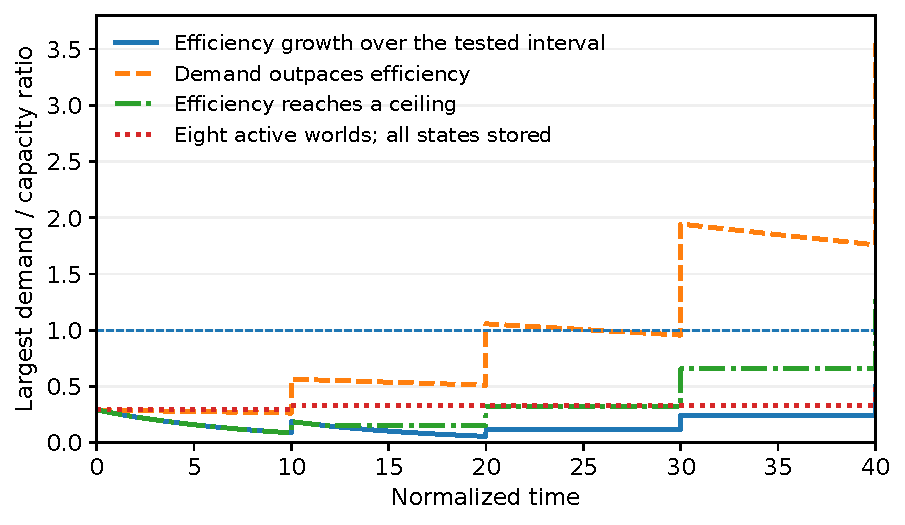
\includegraphics[width=.95\textwidth]{fig1.pdf}
\caption{Finite-horizon local support constructions. The largest service-demand ratio must remain at or below one. Processing and heat are charged to active worlds; persistent memory is charged to all represented states, including inactive ones. Growth in depth is stepwise. No curve is extrapolated to unlimited time, and no physical implementation is validated.}
\label{fig:support}
\end{figure}

\subsection{A joint finite-interval witness}

The support and allocation examples need not be merely disconnected illustrations. Couple the matched-efficiency schedule in \cref{sec:support} to $B=10$, $C_0=0$, $a(t)=W_{d(t)}/\ln(11)$, $r_n=r_h=0.1$, and all three prices equal to one. Set $q=0.99$, $\epsilon_R=\epsilon_I=0.001$, with unit initial slopes for $E,R,I$. At $z=B$, useful computation is exactly $C_L=W_{d(t)}$, the workload charged in the support example. The three outward-to-local marginal-return ratios are
\begin{equation}
 11\ln(11)\left[S_j+\frac{r_j+S_j}{W_{d(t)}}\right],
 \qquad(S_n,S_h,S_m)=(0.012,0.002,0.001).
 \label{eq:joint-witness}
\end{equation}
They decrease with world count and are already below one at seven worlds. Thus this same finite family satisfies both the three-service feasibility test and strict all-inward optimality with positive residual external values. As the hierarchy grows from seven to 127 worlds, attained logarithmic value rises from $\ln8$ to $\ln128$. The budget is fixed at $B=10$ and productivity is deliberately tuned to $a(t)=W_{d(t)}/\ln 11$. This is a consistency witness, not evidence for the plausibility of that productivity path, an engineering implementation, or an infinite-horizon optimum. Persistent memory is still charged to every world; future resource effects are considered separately in \cref{sec:dynamic}.

\subsection{Budget growth and shared technological progress}

With perfect experiential substitution and no residual external value, $q=1$ and $\epsilon_R=\epsilon_I=0$. For \emph{any} strictly increasing $F$, maximizing value is equivalent to maximizing $C$. Let
\begin{equation}
 R_* = \max\{r_n/p_n,r_h/p_h\}.
 \label{eq:Rstar}
\end{equation}
When $R_*>0$, the solution allocates
\begin{equation}
 z^*=\min\{B,\max(a/R_*-1,0)\},\qquad
 B_{\rm crit}=a/R_*-1.
 \label{eq:budgetcrit}
\end{equation}
Any remaining budget goes to a best-return computational external channel. The all-inward condition is $a/(1+B)\geq R_*$. If $R_*=0$, all investment is local. This exposes a limitation of a fixed-budget productivity path: with fixed $a$ and $R_*>0$, a sufficiently large budget restores external investment even without authenticity, information, or resilience premiums. The civilization does not stop preferring more value when it can generate virtual worlds.

If local and remote computational coefficients all receive the same multiplicative improvement, the pure-computation condition is unchanged. Progress that disproportionately raises intensive return can support inward allocation; progress that improves everything equally need not. \Cref{fig:budget} shows this budget effect for $R_*=1$. Persistent inward allocation along a development path requires the relevant inequalities to hold along that path, not merely at one chosen value of $B$.

\begin{figure}[tbp]
\centering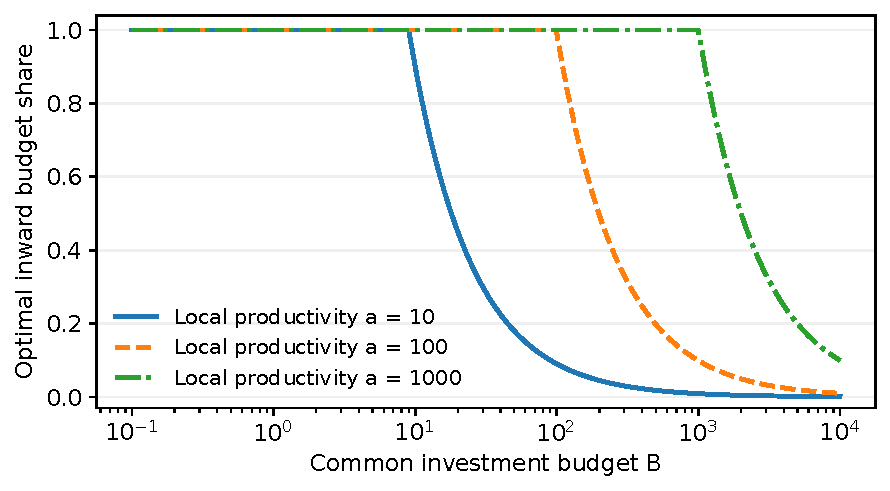
\includegraphics[width=.95\textwidth]{fig2.pdf}
\caption{Exact inward budget share with perfect experiential substitution, zero residual value, and $R_*=1$. The transition occurs at $B=a-1$. Greater local productivity moves the boundary, but budget growth can eventually favor additional external capacity. Any strictly increasing computational value function gives the same allocation in this pure-computation case.}
\label{fig:budget}
\end{figure}

\section{Paired sensitivity design and numerical specification}
\label{supp:paired}\label{sec:access}
\subsection{Paired sensitivity design}
To distinguish deployment costs from access delays, use the normalized
family
\begin{equation}
 p_j=p_{j0}\left(f+\frac{1}{s_t}+\frac{0.2}{s_c}\right),\qquad
 r_j=r_{j0}m_r\exp(-0.1/s_t),\qquad a=a_0m_a.
 \label{eq:speed-map}
\end{equation}
Here $f>0$ is the residual price factor; $s_t,s_c>0$ index effective
material and information access speeds relative to $c$.
At instantaneous access, $p_j=p_{j0}f$ and $r_j=r_{j0}m_r$.
The coefficients $0.2$ and $0.1$ define scenarios, not calibrated physical
laws. Speed sweeps also remove the stipulated attenuation of remote
returns, so they are \emph{not} pure price experiments. The fixed-access
sweeps in $f$ isolate the price effect.

Faster-than-light access is only a counterfactual limiting case of this
map, not a physical mechanism established here. Instantaneous arrival
still leaves the positive deployment price $p_{j0}f$. Exactly zero
external prices are excluded: they can destroy compactness of the
feasible set and, with positive external computational returns and
unbounded increasing value, need not admit a finite optimizer.

The reference design contains 1,024 scrambled Sobol points in 14
dimensions, paired across every scenario. The exact library, generator
call and frozen inputs are specified in \cref{app:numerical}. Marginals
are log-uniform over the stated normalized ranges. The concave residual
benefits are
\begin{equation}
 E(x)=A_E(1-\exp(-x/s_E)),\quad
 R(u)=A_R(1-\exp(-u/s_R)),\quad
 I(v)=A_I(1-\exp(-v/s_I)).
 \label{eq:benefit-family}
\end{equation}
The reference uses $(q,\epsilon_R,\epsilon_I,f)=(0.99,0.01,0.05,1)$
and $m_a=m_r=1$. \Cref{tab:scenarios} retains the full paired counts.

At instantaneous access, the reference has 219 inward corners; a
uniform $10\%$ price cut leaves 207. Only 364 reference inputs admit
a finite productivity threshold with the same residual slopes; the other
660 violate a residual-floor condition. Perfect experiential substitution
with zero residual weights yields 527 inward corners, while 497 still
prefer external computational capacity. Raising only local productivity
tenfold gives 314 inward corners; raising local and remote productivity
together gives 222. At $f=0.01$ and $f=10^{-4}$, the count is zero.
These are exact classifications of the archived inputs, not estimates of
civilizational prevalence.

Eight additional scrambles of 4,096 points each give instantaneous
inward fractions of \DesignLogMin--\DesignLogMax\% under the same
log-uniform marginals. Linear-uniform marginals over the same endpoints
give \DesignLinearMin--\DesignLinearMax\%. These 65,536 classifications
use the exact boundary. Their variation describes sensitivity to the
parameter-space measure, not observational uncertainty about the Galaxy.

\subsection{Frozen design and retained paired results}
\label{supp:legacy-numerical}

The canonical unit points and transformed parameters are the arrays
\texttt{sobol\_vectors} and \texttt{parameters} in
\texttt{data/allocation/design.npz}. The generating environment records
Python~3.13.5, NumPy~2.3.5 and SciPy~1.17.0. The exact call is
\begin{verbatim}
from scipy.stats import qmc
u = qmc.Sobol(d=14, scramble=True,
              seed=20260905).random_base2(m=10)
\end{verbatim}
The default \texttt{bits=None} resolves to 30 bits; optimization is
\texttt{None}. No points are skipped or thinned. For the ordered endpoint
vectors in \cref{tab:ranges}, the transformation is
\begin{verbatim}
lo = np.log(lower_endpoints)
hi = np.log(upper_endpoints)
parameters = np.exp(lo + u * (hi - lo))
\end{verbatim}
Every scenario uses the same transformed rows.

Re-execution in SciPy~1.17.0 reproduces the archived unit points bit for
bit. Floating-point exponentiation changes some transformed entries by
at most a relative $2.22\times10^{-16}$ in the present environment;
all classifications agree. Evaluation of the frozen arrays reproduces
219 instantaneous-reference inward corners and 527 under perfect
substitution with zero residual weights, as well as all other counts
in \cref{tab:scenarios}.

With \texttt{seed=20260905}, the archived unit points are reproduced
bit for bit in the historical checks under SciPy~1.17.0 and 1.18.1;
\texttt{rng=20260905} yields a different scramble, with 208
instantaneous and 530 perfect-substitution inward corners.
The frozen arrays, not the seed alone, define the reference experiment.
The frozen package and the accompanying integrity manifest record the generator and checksums. The present rerun uses SciPy~1.17.0; the 1.18.1 result is retained archival evidence.

The parameter order is $(B,C_0,a,r_n,r_h,A_E,A_R,A_I,s_E,s_R,s_I,p_{n0},p_{h0},p_{m0})$. All base marginal ranges are log-uniform in the reference experiment. The stored columns named e, r, and i are written $s_E,s_R,s_I$ here; their values and ordering are unchanged.

\begin{table}[htbp]
\centering
\caption{Normalized ranges in the 14-dimensional reference design.}
\label{tab:ranges}
\begin{tabular}{@{}lll@{}}
\toprule
Quantity & Range & Meaning\\
\midrule
$B$ & $1$--$100$ & common investment budget\\
$C_0$ & $0.1$--$10$ & existing useful computational service\\
$a$ & $1$--$1000$ & intensive computational coefficient\\
$r_n,r_h$ & $0.1$--$10$ & external computational returns\\
$A_E,A_R,A_I$ & $0.1$--$10$ & benefit amplitudes\\
$s_E,s_R$ & $1$--$30$ & experiential and resilience scales\\
$s_I$ & $1$--$100$ & information scale\\
$p_{n0}$ & $1$--$10$ & resident unit price\\
$p_{h0}$ & $0.1$--$3$ & industry-only unit price\\
$p_{m0}$ & $0.01$--$0.3$ & observation-only unit price\\
\bottomrule
\end{tabular}
\end{table}

The sublight scenario has $(s_t,s_c)=(0.01,1)$, the communication-only variant $(0.01,\infty)$, the light-speed case $(1,1)$, and combined faster-access cases $(10,10)$, $(1000,1000)$, and $(\infty,\infty)$. The no-substitution variant sets $q=0$. Large residual values set $\epsilon_R=\epsilon_I=1$, either retaining $q=0.99$ or additionally setting $q=0$. The two tenfold productivity variants set $(m_a,m_r)=(10,1)$ and $(10,10)$. The perfect-substitution variant sets $(q,\epsilon_R,\epsilon_I)=(1,0,0)$. Reduced-price variants set $f=0.01$ or $10^{-4}$ with instantaneous access; other parameters remain at reference settings. A material-speed variable is not allowed to make numerical prices exactly zero.

\begin{table}[htbp]
\centering\small
\caption{All-inward inputs out of 1,024, with a conditional price-robustness check. The last column applies a uniform 10\% price reduction to each listed scenario while retaining its other settings. It is computed from the exact boundary, not from a new behavioral assumption or an observational sample.}
\label{tab:scenarios}

% BEGIN expanded scenario_table.tex
\begin{tabularx}{\textwidth}{@{}Xrr@{}}
\toprule
Scenario & All inward & Still inward after 10\% price cut \\
\midrule
Sublight material travel & 929 & 923 \\
Fast communication only & 929 & 923 \\
Light-speed limit & 326 & 313 \\
Travel and communication at 10c & 234 & 219 \\
Travel and communication at 1000c & 219 & 207 \\
Instantaneous reference & 219 & 207 \\
No experiential substitution & 146 & 135 \\
Large residual values & 14 & 14 \\
No substitution + large residuals & 11 & 10 \\
Local productivity $\times10$ & 314 & 296 \\
Local and remote productivity $\times10$ & 222 & 211 \\
Perfect substitution; no residual values & 527 & 505 \\
Outward price floor $\times0.01$ & 0 & 0 \\
Outward price floor $\times0.0001$ & 0 & 0 \\
\bottomrule
\end{tabularx}

% END expanded scenario_table.tex

\end{table}

Corner classification uses the exact inequalities, not optimizer-selected shares. The stored optimal shares are checked separately using the objective and concavity certificates described in the archived Supplementary Material and audit outputs. Small platform-dependent changes in transformed parameters or nearly tied optimized shares do not change any archived corner classification in the checks reported here.

For design-measure sensitivity, Sobol seeds 20260911 through 20260918 each generate $2^{12}$ points. Both log-uniform and linear-uniform transformations use the same bounds in \cref{tab:ranges}. Repeated scrambles assess numerical integration stability under a selected measure. They do not supply a prior justified by extraterrestrial observations.


\section{Archived two-period construction}
\label{supp:dynamic}

A one-horizon budget comparison omits one of the strongest reasons to expand: external industry can enlarge future resources. A minimal two-period construction makes this effect explicit while also allowing local investment to be productive. Let $B_1=10$, $z_1=B_1-p_1x$, and define
\begin{align}
 C_1(x)&=C_{01}+a_1\ln(1+z_1)+r_1x,\nonumber\\
 B_2(x)&=B_{20}+g_Lz_1+g_Xx,\label{eq:futurebudget}\\
 W(x)&=\ln[1+C_1(x)]+\beta V_2[B_2(x)],\quad 0\leq x\leq B_1/p_1.
 \label{eq:dynamic}
\end{align}
Here $B_1>0$, $B_{20},C_{01},C_{02}\geq0$, $a_1,a_2,p_1,p_2,r_1,r_2>0$, and $0\leq\beta\leq1$. The parameters $g_L,g_X\geq0$ convert current allocations to next-period resources. Both directions receive a future-production channel. All represented downstream benefits of first-period projects are captured through $B_2$; this is not a full persistent-capital or interstellar replication model.

The continuation value is the second-period pure-computation problem,
\begin{equation}
 V_2(B)=\max_{\substack{z_2,x_2\geq0\\z_2+p_2x_2\leq B}}\ln[1+C_{02}+a_2\ln(1+z_2)+r_2x_2].
 \label{eq:continuation}
\end{equation}
For $r_2>0$,
\begin{equation}
 z_2^*(B)=\min\{B,\max(a_2p_2/r_2-1,0)\},\qquad
 x_2^*(B)=\frac{B-z_2^*(B)}{p_2}.
 \label{eq:stage2}
\end{equation}
Its marginal value $V_2'(B)$ is the current best computational marginal return divided by $1+C_2^*(B)$: $a_2/(1+B)$ on the all-local branch, or $r_2/p_2$ on the mixed/external branch. The expressions agree at the switching budget. $V_2$ is increasing and concave.

The archived specialization of \cref{prop:dynamic} is
\begin{equation}
 \frac{r_1-p_1a_1/(1+B_1)}{1+C_{01}+a_1\ln(1+B_1)}
 +\beta V_2'(B_{20}+g_LB_1)(g_X-p_1g_L)\leq0.
 \label{eq:dynamiccriterion}
\end{equation}
The derivative proof in the main text applies because both current and
continuation objectives here are concave.


The first term is the original within-period comparison. The second values the \emph{difference} between external and local production of future resources. Counting $g_X$ while setting $g_L$ to zero without justification would bias the test against inward development; omitting $g_X$ would bias it in favour. This extension is a structural check, not a calibrated decision rule for actual civilizations.

For $p_1=p_2=r_1=r_2=1$, $a_1=a_2=100$, $C_{01}=C_{02}=B_{20}=1$, $g_L=0.2$, and $\beta=0.9$, present-only investment is all inward. The future-adjusted corner changes at $g_X=\DynamicThreshold$. At $g_X=0.2$ both periods remain all inward. At $g_X=2$, optimal first-period outward investment is $x=\DynamicOutward$, leaving $z_1=6.2441$ locally and producing $B_2=9.7607$. All second-period investment is still local. Thus the optimal path can include \emph{external investment undertaken to finance later inward activity}. This differs from claiming that external expansion is never useful. \Cref{fig:dynamic} gives the full 201-setting construction.

\begin{figure}[tbp]
\centering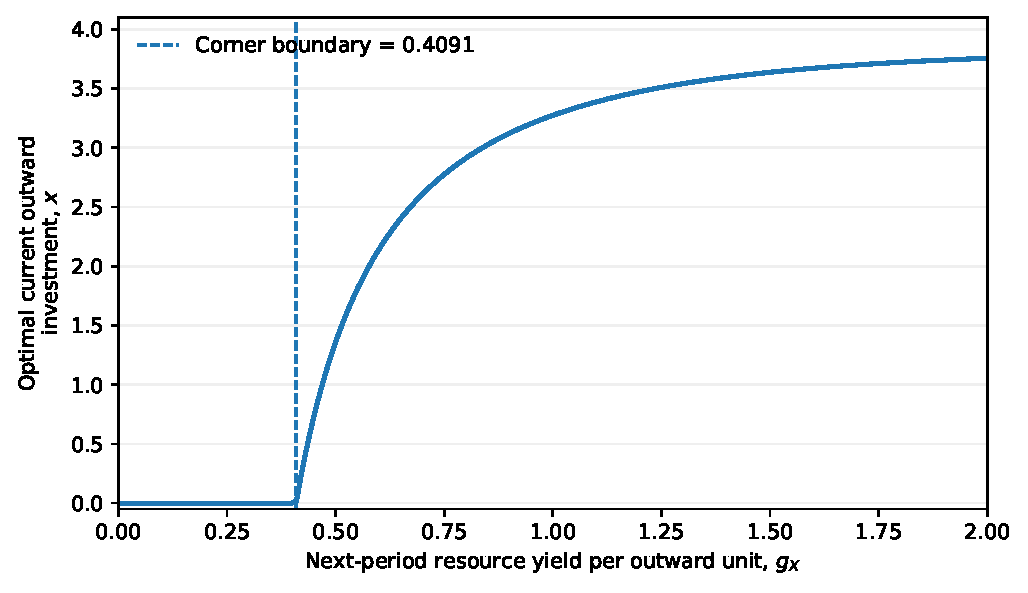
\includegraphics[width=.95\textwidth]{fig4.pdf}
\caption{Two-period resource feedback. Local investment generates future resources at $g_L=0.2$ per unit. Increasing the external yield $g_X$ eventually overturns the all-inward present-only optimum. Parameters are normalized; the transition is an exact derivative boundary checked against a separate three-variable numerical optimization.}
\label{fig:dynamic}
\end{figure}

The converse reversal is also possible. Keep
$B_1=10$, $p_1=p_2=r_1=r_2=1$ and $\beta=0.9$, but set
$a_1=5$, $a_2=100$, $C_{01}=C_{02}=1$, $B_{20}=0$,
$g_L=0.1$ and $g_X=0$. The static term in
\cref{eq:dynamiccriterion} is $\ReverseStaticTerm$, and the
present-only optimum is $x=\ReverseStaticX$. The continuation term is
$\ReverseFutureTerm$, making the total $\ReverseTotalTerm$.
Concavity therefore makes $x=\ReverseDynamicX$ the two-period optimum.
Local investment, rather than external investment, produces the more
valuable continuation budget in this example. Supplementary Material
section~S3 reports scalar and joint-optimization checks of both cases.

The two reversals are retained as finite-horizon examples. The infinite-horizon
benchmark in \cref{prop:infinite} now supplies a separate verification theorem,
with its own production and growth assumptions. The nonlinear examples here
are exact special cases of \cref{prop:dynamic}, not of the linear benchmark.

\section{Additional identities and new verification files}
\label{supp:newchecks}
The workload ratios used in the main text are, explicitly,
\begin{equation}
 \frac{D_k(d+1)}{D_k(d)}=b+\frac1{W_d}\longrightarrow b,
 \label{eq:recursion-cost}
\end{equation}
\begin{equation}
 F(C_{d+1})-F(C_d)=\ln\frac{1+c(bW_d+1)}{1+cW_d}\longrightarrow\ln b.
 \label{eq:recursion-value}
\end{equation}
Their proofs divide by $W_d\to\infty$. A nonconcave example retained from
v7.3 is
\begin{equation}
 U(x)=\ln\{1+2\ln(2-x)+0.1x\}+3x^2,\quad 0\leq x\leq1,
 \label{eq:nonconcave}
\end{equation}
with $U'(0)\simeq-0.3772$, $U(0)\simeq0.8697$, and
$U(1)\simeq3.0953$. It violates the concavity assumption, not the corner theorem.

Each new script in \texttt{code/validate\_v8\_*.py} is self-contained and
prints explicit pass and fail counts. The accompanying README maps files
to propositions and distinguishes assertions from independent randomized
cases; each script records its seed and tolerances. The new no-replication classification reads
\texttt{archive/v7\_3/data/allocation/design.npz} without changing it.
It solves observation on the restricted face, then evaluates the two
replication reduced derivatives; 64 of the 1,024 cases are additionally
compared with full constrained optimization. General restricted-face tests
use 320 separate randomized instances with optional backups. Thus the full
optimization check is sampled, whereas every frozen row receives the exact
face criterion.

The original archive scripts have been rerun in a working copy, not in the
immutable archive. Their outputs are included under
\texttt{results/archive\_rerun/}. No figures or archived classification
counts have been revised. Mechanical source and PDF checks are recorded in
\texttt{results/assembly\_audit.json} and
\texttt{results/final\_audit.json}; physical-parameter sources are documented
in the comments of \texttt{code/validate\_v8\_7\_physical.py}.
The finite-efficiency tests are in \texttt{code/validate\_v8\_8\_ceiling.py}
and \texttt{results/v8\_8\_ceiling.json}.

\end{document}
